%% Semantic Assistants Documentation
%% 
%% This file is part of the Semantic Assistants architecture.
%%
%% Copyright (C) 2009, 2010, 2011 Semantic Software Lab, http://www.semanticsoftware.info
%%
%% The Semantic Assistants architecture is free software: you can
%% redistribute and/or modify it under the terms of the GNU Affero General
%% Public License as published by the Free Software Foundation, either
%% version 3 of the License, or (at your option) any later version.
%% 
%% This program is distributed in the hope that it will be useful,
%% but WITHOUT ANY WARRANTY; without even the implied warranty of
%% MERCHANTABILITY or FITNESS FOR A PARTICULAR PURPOSE.  See the
%% GNU Affero General Public License for more details.
%% 
%% You should have received a copy of the GNU Affero General Public License
%% along with this program.  If not, see <http://www.gnu.org/licenses/>.
%%

\documentclass[10pt,twoside,openany,bibtotoc,liststotoc,chapterprefix]{scrbook}
\usepackage{microtype}
\usepackage{bookman}
\usepackage{color}
\usepackage{url}
\usepackage{rotating}
\usepackage{listings}
\usepackage{booktabs}
\usepackage{amsmath}
\usepackage{hyperref}
\usepackage{xspace}
%\usepackage{html}
\usepackage[round, sort]{natbib}

%% package options
% KOMA-Script
\typearea{12}
%%%%%%%%%%%%%%%%%%%%%%%%%%%%%%%%%%%%%%%%%%%%%%%%%%%%%%%%%%%%
%
%  Adding lines above and below the chapter head
%
 
% 1st get a new command
\newcommand*{\ORIGchapterheadstartvskip}{}%
% 2nd save the original definition to the new command
\let\ORIGchapterheadstartvskip=\chapterheadstartvskip
% 3rd redefine the command using the saved original command
\renewcommand*{\chapterheadstartvskip}{%
  \ORIGchapterheadstartvskip
  {%
    \setlength{\parskip}{0pt}%
    \noindent\rule[.3\baselineskip]{\linewidth}{1pt}\par
  }%
}
 
% see above
\newcommand*{\ORIGchapterheadendvskip}{}%
\let\ORIGchapterheadendvskip=\chapterheadendvskip
\renewcommand*{\chapterheadendvskip}{%
  {%
    \setlength{\parskip}{0pt}%
    \noindent\rule[.3\baselineskip]{\linewidth}{1pt}\par
  }%
  \ORIGchapterheadendvskip
}
%
%  End of chapter head change
%
%%%%%%%%%%%%%%%%%%%%%%%%%%%%%%%%%%%%%%%%%%%%%%%%%%%%%%%%%%%%

%% floats
\setcounter{topnumber}{2}
\setcounter{bottomnumber}{1}
\renewcommand{\floatpagefraction}{0.9}
\renewcommand{\topfraction}{0.9}
\renewcommand{\bottomfraction}{0.9}
\renewcommand{\textfraction}{0.1}

%% color definitions
\definecolor{darkred}{rgb}{0.5,0.0,0.0}
\definecolor{darkgreen}{rgb}{0.0,0.4,0.0}
\definecolor{darkblue}{rgb}{0.0,0.0,0.5}
\definecolor{gray}{gray}{0.8}
\addtokomafont{sectioning}{\color{blue}}

%% listing
\lstloadlanguages{Lisp,Java,Make,Ant}
\lstset{language=XML,
        basicstyle=\footnotesize\sffamily, %\ttfamily,
        keywordstyle=\color[rgb]{0.5,0,0.33203125}\bfseries,
        frame=shadowbox,
        rulesepcolor=\color{gray},
        commentstyle=\color[rgb]{0.24609375,0.5,0.37109375}, % commentstyle=\color{blue}\textit,
        extendedchars=true,
        showstringspaces=false,
        breaklines=true,
        breakatwhitespace=false,
        showlines=true,
        backgroundcolor=\color{white},
        numberstyle=\scriptsize,
        stepnumber=1,
        numbersep=5pt,
        numbers=left,
        stringstyle=\color[rgb]{0.1640625,0,1}\ttfamily}
%% url
\urlstyle{same}

%% hyperref
\hypersetup{
  backref=true,
  colorlinks=true,
  citecolor=darkgreen,
  linkcolor=darkred,
  urlcolor=darkblue,
  filecolor=red,
  letterpaper=false,
  bookmarks=true,
  bookmarksopen=true,
  pdfpagemode=UseOutlines,
  pdftitle={Semantic Assistants Documentation}, 
  pdfauthor={Semantic Software Lab}
}

\newcommand{\blankline}{\vspace{5mm}}

%\begin{comment}
%% miscellaneous macros
\newcommand{\sfcap}[1]{\strut\vspace*{-1mm}{\footnotesize\textsf{#1}}}
\newcommand{\filetilde}{\char126$\!\!$}
\newcommand{\javadoc}[1]{\begin{tabular}{|l|}\hline
  \textbf{Visit the JavaDoc Documentation}\\
  \url{#1}\\ 
  \hline\end{tabular}}
\newcommand{\argmax}{\mathop{\mathrm{argmax}}}
\newcommand{\sa}{Semantic Assistants\xspace}

\newcommand{\wikinlp}{Wiki-NLP\xspace}

\title{Semantic Assistants\bigskip\\
\Large Guide for Users and Developers}
\author{Ren\'{e} Witte\\
Thomas Gitzinger\\
Nikolaos Papadakis\\
Bahar Sateli\\
Elian Angius
\medskip}
\date{Development Release\\
\today
}
\publishers{Semantic Software Lab\\
Concordia University\\
Montr\'{e}al, Canada\\
{\large\url{http://www.semanticsoftware.info}}
}

\begin{document}
\frontmatter
\maketitle

% Table of Contents
\pdfbookmark{Contents}{2}\tableofcontents

\section*{About this document}
This document contains documentation for the \emph{Semantic
  Assistants} project. You can obtain the latest version from
\url{http://www.semanticsoftware.info/semantic-assistants}. The source
code is hosted on SourceForge,
\url{https://sourceforge.net/projects/semantic-assist/}.  A public
Jenkins server is hosted on
\url{http://assistant.semanticsoftware.info}.

\section*{Acknowledgments}
The following developers contributed to the design and implementation
of the Semantic Assistants: Ren\'{e} Witte, Tom Gitzinger, Nikolaos
Papadakis, Bahar Sateli. Additional thanks to Ninus Khamis for
his contributions.

\section*{Licenses}
The Semantic Assistants architecture, clients, and resources are
published under the GNU Affero General Public License v3
(AGPL3).\footnote{AGPL3,
  \url{http://www.gnu.org/licenses/agpl-3.0.html}} Exceptions are the
Client-Side Abstraction Layer, which is licensed under the  LPGL3.\footnote{LGPL3, \url{http://www.gnu.org/licenses/lgpl-3.0.html}}

This product also includes software developed by the Apache Software
Foundation (\url{http://www.apache.org/}), licensed under the Apache
Software License, Version 1.1.

The included NLP pipelines also contain code from the GATE project
(\url{http://gate.ac.uk}) licensed under the LPGL3.\footnote{LGPL3, \url{http://www.gnu.org/licenses/lgpl-3.0.html}}

The Semantic Assistants server utilizes libraries from the Pro\'eg\'e
project, which are licensed under the Mozilla Public license
(MPL).\footnote{Mozilla Public License (MPL),
  \url{http://mozilla.org/MPL/MPL-1.1.html}} Additionally, it uses
the Jena framework for Java and International Components for Unicode Java library; please refer to the license files included with
the distribution files or the Jena\footnote{Jena License and
  Copyright, \url{http://jena.sourceforge.net/license.html}} and icu4j\footnote{icu4j Copyright and Permission Notice, \url{http://www.xom.nu/lib/normalizer_license.html}} Websites for details.

\mainmatter
\part{Introduction}
%% Semantic Assistants Documentation
%% 
%% This file is part of the Semantic Assistants architecture.
%%
%% Copyright (C) 2009, 2010, 2011 Semantic Software Lab, http://www.semanticsoftware.info
%%
%% The Semantic Assistants architecture is free software: you can
%% redistribute and/or modify it under the terms of the GNU Affero General
%% Public License as published by the Free Software Foundation, either
%% version 3 of the License, or (at your option) any later version.
%% 
%% This program is distributed in the hope that it will be useful,
%% but WITHOUT ANY WARRANTY; without even the implied warranty of
%% MERCHANTABILITY or FITNESS FOR A PARTICULAR PURPOSE.  See the
%% GNU Affero General Public License for more details.
%% 
%% You should have received a copy of the GNU Affero General Public License
%% along with this program.  If not, see <http://www.gnu.org/licenses/>.
%%

\chapter{Introduction to Semantic Assistants}

\section{Overview}
The \sa project aims to bring natural language processing (NLP)
techniques directly to end users by integrating them with common
desktop applications, such as word processors, email clients, or Web
browsers. To facilitate the connection between NLP frameworks and
(desktop) clients, a service-oriented architecture
(Figure~\ref{fig:arch}) has been developed that allows to integrate
(desktop) clients with NLP services implemented in the GATE
framework.\footnote{GATE, \url{http://gate.ac.uk}} NLP services are
published as standard Web services with a WSDL description.

For the general motivation, design, and background on the \sa project,
please read the information on the \sa Web site\footnote{Semantic
  Assistants,
  \url{http://www.semanticsoftware.info/semantic-assistants}} and the
contained references first \citep{giwi08,aswc08}. This document only
describes the installation and use of the developed system.

\begin{figure}[t]
  \centering
  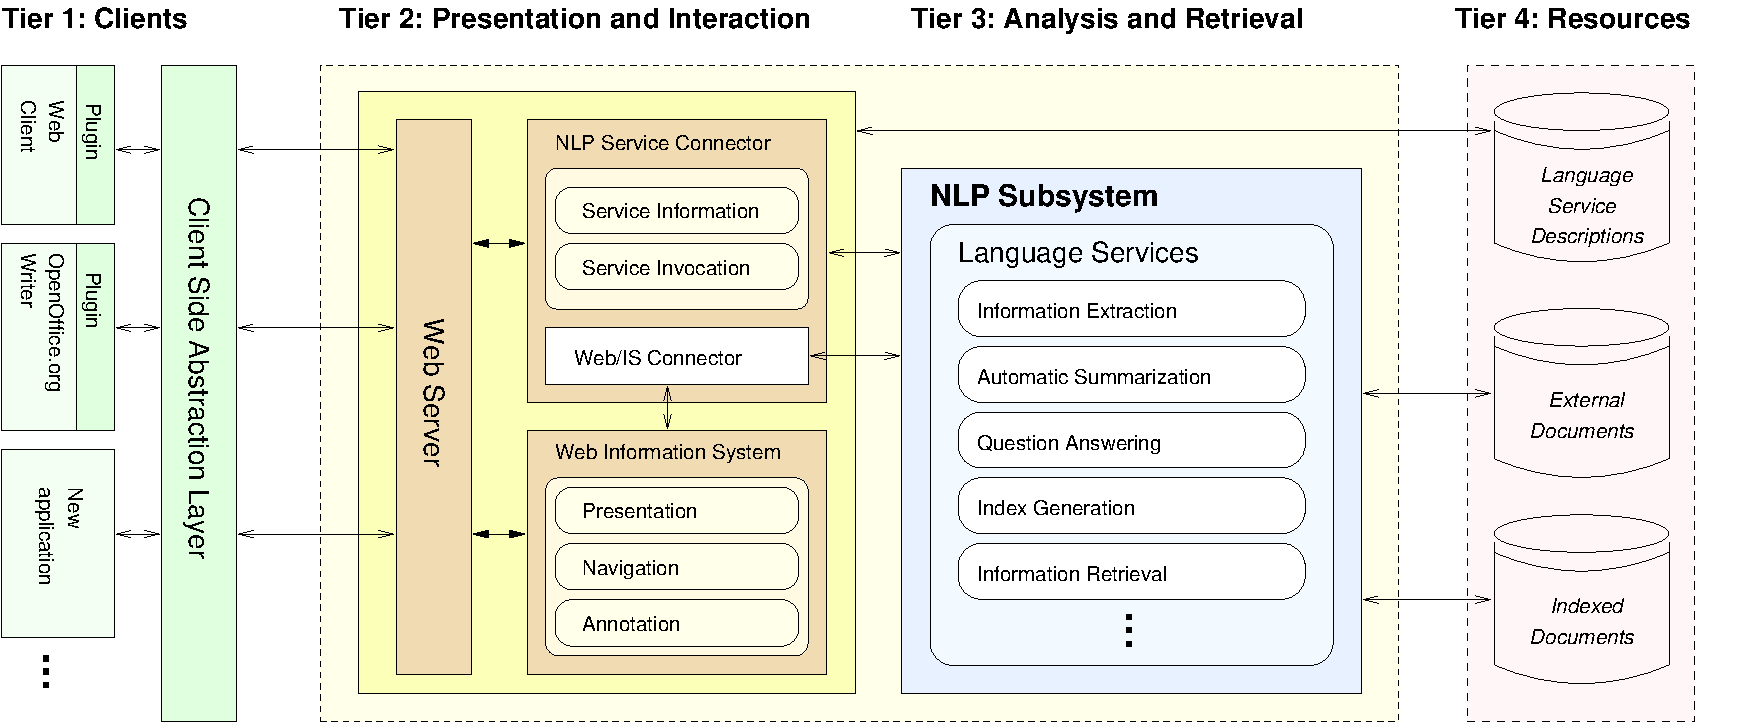
\includegraphics[width=\textwidth]{pictures/arch}
  \caption{The \sa architecture}
  \label{fig:arch}
\end{figure}

\section{How to read this documentation}
To deploy \sa, we recommend you first read this overview chapter.
Then, consult the following parts of this documentation:

\begin{description}
\item[End Users:] Please refer to the installation guide in
  Chapter~\ref{chap:inst}, as well as the client-specific installation
  instructions in Chapter~\ref{chap:clients}. Additionally, if you
  want to run your own server, read the server installation guide
  (Chapter~\ref{chap:serv}).

\item[Language Engineers:] If you want find out how to integrate a
  GATE pipeline as a new NLP service, please refer to
  Chapter~\ref{chap:services} for documentation on the OWL service
  descriptions and Section~\ref{sec:nlpservices} for publishing the
  new service through the \sa server.

\item[Plug-in Developers:] Please first read the background material
  (Web site, papers). Then refer to the developers' notes in
  Chapter~\ref{chap:dev}.
\end{description}

\section{Architectural Overview}
\label{sec:implementation}
This section gives an overview over the current version of the Semantic
Assistants architecture, as shown in Figure~\ref{fig:arch}:

\paragraph{Tier 1} of the architecture consists of client applications
and a \emph{Client-Side Abstraction Layer (CSAL)}. Currently, there
are two example clients distributed with the system, a simple
command-line client for testing purposes and a plug-in for the
OpenOffice.org \emph{Writer} word processor. The client-side abstraction
layer consists partly of hand-written Java classes that provide
common client-side functionality, partly of automatically generated
Java classes. The communication between client and server is
implemented by means of W3C Web services.\footnote{Web Services Architecture, see
  \url{http://www.w3.org/TR/ws-arch/}} 

\paragraph{Tier 2} of the architecture consists of a \emph{Web server}
and the \emph{NLP Service Connector}. The Web server used by default
in the architecture is the Java~6 embedded Web server.  The NLP
Service Connector currently integrates the GATE framework for NLP. It
is responsible for a number of tasks, including communication with the
client, reading and querying the language service descriptions,
running requested language services, and generating response messages.

\paragraph{Tier 3} is the NLP subsystem. At present, only the GATE
framework is supported (future work might integrate additional
frameworks, such as UIMA).  It makes use of the GATE API in order to
assemble language services, store them in a permanent way, and invoke
them when they are requested by a client.

\paragraph{Tier 4} is the resource tier.  Here we have the language
service descriptions, which are authored in the Web Ontology Language
(OWL).  Tier~4 further contains external documents, which the NLP
subsystem must be able to access. Finally, we possibly have
pre-indexed documents as part of the resources tier. For indexing,
GATE uses Apache's Lucene indexer\footnote{Apache Lucene, see
  \url{http://lucene.apache.org/}} as a subsystem, and allows us,
through its API, to create and access indices.


\section{System Components}
\label{sec:syscomp}
The implementation of the Semantic Assistants architecture currently comes
with the following components:

\begin{description}
\item[Server:] The server is the core of the architecture.  It
  communicates with the clients through the CSAL on one hand and
  the NLP framework through the NLP Service Connector on the other.
  At present, the architecture only contains a connector for
  GATE. However, it was explicitly designed to allow an easy
  integration of other frameworks (for example, UIMA). For describing
  available services, we use ontology-based (OWL) service
  descriptions. As a service-oriented architecture (SOA), every
  service is automatically available to all clients connected to the
  architecture, using standard WSDL\footnote{Web Services Description
    Language (WSDL), see \url{http://www.w3.org/TR/wsdl}}) interface
  descriptions.

\item[Client-Side Abstraction Layer (CSAL):] Our top goal was to make
  it as easy as possible for client (plug-in) developers to integrate
  NLP functionality. As clients should be able to connect to the
  architecture entirely by ``local'' means, we provide an
  \emph{abstraction layer}, named CSAL, which is located on the client
  side and performs the actual communication with the server.

  Apart from the communication functionality, the CSAL also provides
  common client-side functionality, i.e., useful data types and
  methods that are frequently required when integrating NLP into
  desktop clients.

\item[Clients:] Two example clients come with the architecture: a
  command-line client and a plug-in for the OpenOffice.org Writer word
  processor. 

\item[Example Resources:] NLP functionality is provided to clients
  through Web services. To match clients with suitable services
  (depending on language, formats, etc.), each NLP service comes with
  a semantic service description in OWL format. Three example service
  descriptions are included in the current distribution: an
  information extraction (IE) service that detects persons and locations
  (using GATE's ANNIE pipeline), an IR service (using the Yahoo PR)
  and a compound service, which combines the IR and the IE
  service. These should help you in defining your own NLP services
  that you deliver to your end users (e.g., summarization,
  question-answering, domain-specific NLP services).

\item[Documentation and Online Resources:] Apart from this guide, a
  number of publications on the \sa are available
  online,\footnote{\sa,
    \url{http://www.semanticsoftware.info/semantic-assistants}} as
  well as a discussion forum for support.
\end{description}


% \begin{figure}
%   \centering
%   %\vspace*{-9mm}
%   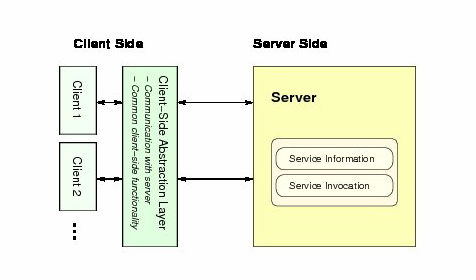
\includegraphics[width=0.6\textwidth]{pictures/abstraction.jpg}
%   \caption{We introduce a client-side abstraction layer}
%   \label{fig:abstraction}
%   %\vspace*{-0.4cm}
% \end{figure}

\section{Example NLP Services}
A number of example pipelines (NLP services) come with the architecture.
They are located in the \url{Resources} directory. There are two
parts: the semantic service descriptions in OWL format stored in the
\url{OwlServiceDescriptions} directory and corresponding GATE
pipelines (\url{.xgapp} files) implementing these services in the
\url{GatePipelines} directory.

\paragraph{Person and Location Extractor.} This NLP service runs the
ANNIE IE system that comes with the standard GATE distribution.  It
detects a number of named entities, such as persons, locations,
organizations, etc.  An OWL service description for this pipeline is
already implemented and stored in the directory
\url{Resources/OwlServiceDescriptions/annie.owl}.  For details on the
OWL-based description format, please refer to Section~\ref{sec:owl}.

\paragraph{Yahoo Search.} This service performs a Web search for a
user and returns the first $n$ documents (where $n$ is a
user-configurable runtime parameter). While this service usually works
as provided, you should obtain a Yahoo API key (see the
\href{http://gate.ac.uk/sale/tao/splitch19.html#x24-51700019.7}{GATE
  manual} for details on this) and store this key in the file
\url{Resources/GatePipelines/Yahoo/application.xgapp} by replacing the
string ``insertyahooidhere'':
\begin{verbatim}
    <string>applicationID</string>
    <string>insertyahooidhere</string>
\end{verbatim}

\paragraph{Web IR Extractor.} The third example service shows how to
combine two existing services, by first calling the Yahoo IR service
and then using the search results as input to the ANNIE IE
service. This service is located in \url{yahooExtractor.owl}.



% Semantic Assistants - http://www.semanticsoftware.info/semantic-assistants

% This file is part of the Semantic Assistants architecture.

% Copyright (C) 2009, 2010, 2011 Semantic Software Lab, http://www.semanticsoftware.info
% The Semantic Assistants architecture is free software: you can
% redistribute and/or modify it under the terms of the GNU Affero General
% Public License as published by the Free Software Foundation, either
% version 3 of the License, or (at your option) any later version.
   
% This program is distributed in the hope that it will be useful,
% but WITHOUT ANY WARRANTY; without even the implied warranty of
% MERCHANTABILITY or FITNESS FOR A PARTICULAR PURPOSE.  See the
% GNU Affero General Public License for more details.
 
% You should have received a copy of the GNU Affero General Public License
% along with this program.  If not, see <http://www.gnu.org/licenses/>.

\chapter{Installation}
\label{chap:inst}
\emph{Note: at present, the installation has been tested under
  Linux and Mac OS X}

\section{Download}
To download the latest version of the \sa and this documentation
please refer to
\url{http://www.semanticsoftware.info/semantic-assistants-architecture}.
A pre-compiled build of the latest version is available from our
Jenkins server, \url{http://assistant.cs.concordia.ca:8080/}. In the
following, we assume you use a pre-compiled version; for compilation
instructions, please refer to Chapter~\ref{chap:dev}.

\section{Prerequisites}
To deploy the \sa architecture, a number of other (open source)
components are needed:

\paragraph{Common throughout the Project:}
\begin{enumerate}
%  \item  Apache ANT, \url{http://ant.apache.org/}
  \item  Sun JDK 6 or newer, \url{http://java.sun.com/javase/downloads/index.jsp}
  \item  GATE v7.0, \url{http://gate.ac.uk/}
\end{enumerate} 

\paragraph{For the \sa Server:}
\begin{enumerate}
  \item Java API for XML Web Services (JAX-WS) v2.1.x, \url{https://jax-ws.dev.java.net/}
%  \item Prot\'{e}g\'{e}-OWL API v3.4, \url{http://protege.stanford.edu/plugins/owl/api/} 
\end{enumerate}

\paragraph{For the CSAL:}
\begin{enumerate}
  \item Java API for XML Web Services (JAX-WS) v2.1.x, \url{https://jax-ws.dev.java.net/}
\end{enumerate}

\paragraph{For the OpenOffice.org Writer Plug-in:}
\begin{enumerate}
\item OpenOffice 3.2, \url{http://download.openoffice.org/}
\item The OpenOffice.org 3.2 SDK,
  \url{http://download.openoffice.org/sdk/index.html}
%\item Apache log4j v1.2,
%  \url{http://logging.apache.org/log4j/1.2/index.html}
%\item Apache Commons Lang v2.4, \url{http://commons.apache.org/lang/}
\end{enumerate}

\paragraph{For the Eclipse Plug-in:}
\begin{enumerate}
\item Eclipse Classic 3.5+ \url{http://www.eclipse.org/downloads/}
\end{enumerate}

%\paragraph{For the Extension for Mozilla Firefox and Mozilla Thunderbird:}
%\begin{enumerate}
%  \item Mozilla Firefox 3.6.x and later \url{http://www.mozilla.org/firefox/} (Earlier versions may work, but are untested.)
%  \item Mozilla Thunderbird 3.1.x and later \url{http://www.mozilla.org/thunderbird/} (Earlier versions may work, but are untested.)
%\end{enumerate}


\section{Path Configuration}
\label{sec:props}
The \emph{SemassistProperties.xml} file serves for two purposes.  It's
included by the ANT \emph{build.xml} files of all projects and
contains common directory paths and used to compile the various
Semantic Assistants components. Secondly, it used by the server at
run-time as a property file.

Users needs to modify the values of the properties in order to
correspond at the proper paths of their machine. The options to be
adapted, include the path to the service description directory, GATE
home, GATE plug-ins, etc. Descriptions of these properties are as the
followings:

The first part is an import statement, where it includes the
\texttt{LocalProperties.xml} file. This file the is the place to store
your local paths and customizations, e.g., you can add additional paths
for your local pipelines in this file.
\begin{lstlisting}[language=XML,numbers=left,xleftmargin=8mm,columns=flexible]
    <!-- Importing LocalProperties.xml file for local paths and customizations -->
    <import file ="LocalProperties.xml"/>
\end{lstlisting}
By default, \texttt{LocalProperties.xml} contains the path to the directory containing the NLP
service descriptions (OWL files):
\begin{lstlisting}[language=XML,numbers=left,xleftmargin=8mm,columns=flexible]
  <property name="service.repository"       value="${semassist.home}/Resources/OwlServiceDescriptions/"/>

  <path id="localruntimeclasspath">
    <!-- Added locally needed paths here -->
  </path>
\end{lstlisting}


The second part of the \texttt{SemassistProperties.xml} is where the
machine-specific variables are modified to point to proper paths of
the users' machine. The variables as follows:
\begin{lstlisting}[language=XML,numbers=left,xleftmargin=8mm,columns=flexible]
    <!-- Machine dependent properties.Need to be modified -->
    <property name="durmtools"          value="/usr/local/durmtools" />
    <property name="jaxws.home"         value="${durmtools}/jaxws-ri" />
    <property name="gate-home"          value="${durmtools}/GATE/gate" />
    <property name="jdk.home"           value="${durmtools}/jdk" />
\end{lstlisting}

\begin{enumerate}
\item \url{durmtools}: This is one of the most important variables in this properties file and needs to be defined properly. According to the prerequisites mentioned earlier, there are various applications that need to be installed prior to using the Semantic Assistants.
Create a folder called \texttt{durmtools} and install all the required applications to this folder, or point this variable to where all your applications are installed e.g. \emph{Applications} on Mac or \emph{Programs} in Windows.
%\item \url{semassist.home}: This variable points to the place on your local machine that the Semantic Assistants package has been downloaded and extracted. Put the full path of the folder in here, exempting the user home directory path for it will be automatically replaced by \texttt{\$\{user.home\}}.
%\item \url{csal.home}: This variable points to the \texttt{CSAL} folder inside the Semantic Assistants package. If the structure is untouched, the path should read \texttt{"\$\{semassist.home\}/CSAL"}.
\item \url{jaxws.home}: This variable points to the Java API for XML Web Services (JAX-WS) v2.1.x application installed in the path defined in \texttt{\$\{durmtools\}} variable.
%\item \url{protege-home}: This variable points to the Prot\'{e}g\'{e}-OWL API v3.4 application installed in the path defined in \texttt{\$\{durmtools\}} variable.
\item \url{gate-home}: This variable points to the GATE v6.0 or newer application installed in the path defined in \texttt{\$\{durmtools\}} variable.
\item \url{jdk.home}: This variable points to the Sun JDK 6 installed on your machine.
\end{enumerate}


The third part includes all the properties used by the OpenOffice.org Writer plug-in. Therefore, in order to use this plug-in, all these variables should be defined beforehand.
\begin{lstlisting}[language=XML,numbers=left,xleftmargin=8mm,columns=flexible]
    <!-- Used by Open Office Writer Plug-In-->    
    <property name="office.home.dir"          value="${durmtools}/OpenOffice"/>
    <property name="uno-copy-dest"  	      value="${user.home}/Documents/uno-components" />
    <property name="office.program.dir"       value="${office.home.dir}/program"/>
    <property name="ooo-classes-basis"        value="${office.home.dir}/basis3.2/program/classes/" />
    <property name="ooo-classes-common"       value="${office.home.dir}/ure/share/java/" />
\end{lstlisting}
\begin{enumerate}
\item \url{office.home.dir}: This variable points to the OpenOffice 3.2 application installed in the path defined in \texttt{\$\{durmtools\}} variable explained earlier.
\item \url{uno-copy-dest}: This variable identifies where the Semantic Assistants plug-in will be stored when it is successfully built. 
\item \url{office.program.dir}: This variable points to the \texttt{program} folder inside \texttt{\$\{office.home.dir\}} path which contains the Writer program.
\item \url{ooo-classes-basis}: This variable points to the folder that contains the bulk, brand-independent OpenOffice functionalities.
\item \url{ooo-classes-common}: This variable points to the folder that containes common Java JAR libraries used by OpenOffice.
\end{enumerate}

The next part includes all the properties used by the Eclipse plug-in. Therefore, in order to use this plug-in, all these variables should be defined beforehand.
\begin{lstlisting}[language=XML,numbers=left,xleftmargin=8mm,columns=flexible]
    <!-- Used by Eclipse Plug-In-->
    <property name="eclipse.program.dir"      value="${durmtools}/eclipse-4.0"/>
    <property name="eclipse.plugins"          value="${eclipse.program.dir}/plugins"/>
\end{lstlisting}
\begin{enumerate}
\item \url{eclipse.program.dir}: This variable points to the Eclipse v3.5 or newer application installed in the path defined in \texttt{\$\{durmtools\}} variable explained earlier.
\item \url{eclipse.plugins}: This variable points to the \texttt{plugins} folder located inside the Eclipse application installed on your machine.
\end{enumerate}

The last part includes all the properties used by the Semantic Assistants server at runtime.
\begin{lstlisting}[language=XML,numbers=left,xleftmargin=8mm,columns=flexible]
    <!-- Used by the server at runtime as properties -->
    <property name="gate.plugin.dir"          value="${gate-home}/plugins/"/>
    <property name="gate.user.file"           value="${semassist.home}/Server/gate-home/user-gate.xml" />
    <property name="ontology.repository"      value="${semassist.home}/Resources/ont-repository/" />
    <property name="gate.pipeline.repository" value="${semassist.home}/Resources/GatePipelines/" />

    <property name="runtime.maxmem"       value="1638m" />
    <property name="runtime.heap.initial" value="128m" />
    <property name="runtime.heap.max"     value="1638m" />
    
    <!-- Server Property Settings (ie # of Threads allowed) -->
    <property name="server.threads.allowed"        value="10"/>

    <property name="server.pipeline.1.name"        value="ANNIE"/>
    <property name="server.pipeline.1.number.pooled"        value="1"/>
    <property name="server.pipeline.1.max.concurrent"        value="1"/>
    <property name="server.pipeline.1.startup"        value="true"/>
    <property name="server.pipeline.1.fullpath"        value="${gate.pipeline.repository}/Annie/"/>

    <property name="server.pipeline.2.name"        value="Organism"/>
    <property name="server.pipeline.2.number.pooled"        value="1"/>
    <property name="server.pipeline.2.max.concurrent"        value="1"/>
    <property name="server.pipeline.2.startup"        value="true"/>
    <property name="server.pipeline.2.fullpath"        value="${gate.pipeline.repository}/OrganismTagger/"/>

    <!-- Port for which the Server listens for debugers to be attached -->
    <property name="server.port.debug"    value="8885"/>
    
    <!-- Port used by the Server to communicate with the clients through wsdl-->
    <property name="server.port.wsdl"     value="8879"/>
\end{lstlisting}
\begin{enumerate}
\item \url{gate.plugin.dir}: This variable points to the GATE application \texttt{plugins} folder used for service executions.
\item \url{gate.user.file}: This variable points to the GATE application user configuration file.
%\item \url{service.repository}: This variable points to the OWL service description files. New service description files are added to this folder once they're available and will be later detected by the server. 
\item \url{ontology.repository}: This variable points to the folder containing the SemanticAssistants OWL files.
\item \url{runtime.maxmem}: This variable contains the maximum amount of runtime memory used by JDK. Unless your JDK complains about the value, leave this as it is.
\item \url{runtime.heap.initial}: This variable contains the initial amount of heap space used by JDK at runtime.
\item \url{runtime.heap.max}: This variable contains the maximum amount of heap space used by JDK at runtime.
\item \url{server.threads.allowed}: This variable contains the number of threads the server should allow to run concurrently.
\item \url{server.pipeline.\#.name}: This variable contains the name of one of the pipelines that will be initialized with certain constraints.  The value must match the actual name of the pipeline used by GATE. (\# must be replaced with an positive integer value.  this number will identify the group of properties related to the pipeline)
\item \url{server.pipeline.\#.number.pooled}: This variable contains the number of threads we wish to keep in memory and allow to be executed concurrently.  Any additional thread of this type will be placed in a queue and will be executed as soon as an available pipeline is free. (\# must be replaced with an positive integer value.  this number will identify the group of properties related to the pipeline)
\item \url{server.pipeline.\#.max.concurrent}: This variable contains the number of maximum threads we will allow to be executed at one time.  The value can be equal to or greater than the \url{server.pipeline.\#.number.pooled} variable.  Once the threads are complete, the number of threds that surpass the \url{server.pipeline.\#.number.pooled} value will be removed from memory
\item \url{server.pipeline.\#.startup}: This variable contains the property that inidicates if this pipeline should be launched at server startup.  This should be set to true in the case that the pipeline you are requesting may take a longer period to ready itself  (\# must be replaced with an positive integer value.  this number will identify the group of properties related to the pipeline)
\item \url{server.pipeline.\#.fullpath}: This variable contains the location of the pipeline application xgapp file.  This is needed to identify the correct pipeline to be executed by the threads (\# must be replaced with an positive integer value.  this number will identify the group of properties related to the pipeline)
\begin{itemize}
  \item It should be noted that if we set the \url{server.pipeline.\#} property in the SemassistProperties.xml file we need to have all 5 properties set correctly.  Each of those properties will be used to set up the pipelines at server startup.
\end{itemize}
\item \url{server.port.debug}: This variable contains the port number on users machine on which the server listens for debuggers to be attached.
\item \url{server.port.wsdl}: This variable contains the port number on which the server communicates with the clients through WSDL.
\end{enumerate}


\section{Client Installation}
The installation and configuration of clients is covered in
Part~\ref{part:desktop} for desktop clients and Part~\ref{part:web}
for web information systems.

\begin{description}
\item[Command-Line Client:] For information on how to compile and run
  the command-line client, please refer to Section~\ref{sec:sacl:clc}.

\item[The OpenOffice.org Writer Plug-In:] For details on how to
  compile and run the OpenOffice.org Writer plug-in please refer to
  Section~\ref{subsec:oo-inst}.

\item[The Eclipse Plug-In:] For details on how to
  compile and run the Eclipse plug-in please refer to
  Section~\ref{subsec:eclipse_install}.

\item[Wiki Systems:] For configuring a MediaWiki installation to run
  SA services, please see Chapter~\ref{chap:wiki}.

\item[Web Portals:] For installing the \sa integration on a Liferay-based portal, please see Chapter~\ref{chap:liferay}.
\end{description}










\part{SA Desktop}
% Semantic Assistants - http://www.semanticsoftware.info/semantic-assistants

% This file is part of the Semantic Assistants architecture.

% Copyright (C) 2009, 2010, 2011 Semantic Software Lab, http://www.semanticsoftware.info
% The Semantic Assistants architecture is free software: you can
% redistribute and/or modify it under the terms of the GNU Affero General
% Public License as published by the Free Software Foundation, either
% version 3 of the License, or (at your option) any later version.
   
% This program is distributed in the hope that it will be useful,
% but WITHOUT ANY WARRANTY; without even the implied warranty of
% MERCHANTABILITY or FITNESS FOR A PARTICULAR PURPOSE.  See the
% GNU Affero General Public License for more details.
 
% You should have received a copy of the GNU Affero General Public License
% along with this program.  If not, see <http://www.gnu.org/licenses/>.

\chapter{\sa Clients}\label{chap:clients}

\section{Command-Line Client}
\label{sec:sacl:clc}
This is a simple example client to access the server from the command line.
It is located under \url{SemanticAssistants/Clients/CommandLine} and is meant to demonstrate and test to plug-in developers various Semantic Assistant functionalities.

\begin{enumerate}
\item To compile: \emph{ant compile}
\item To run: \emph{./runclient.sh}
\end{enumerate}

The \texttt{runclient.sh} script helps with the
class path setting, but also adds some difficulty with getting quotes right
when passing parameters to the program. For example, to list all
available services, you can run
\begin{verbatim}
    ./runclient.sh listall
\end{verbatim}
to query the server for all available NLP services. For the default
installation, you should see an output like:
\begin{verbatim}
    Retrieving service info from server...   done
    Listing services:
    Yahoo Search
    IR Information Extractor
    Person and Location Extractor
\end{verbatim}
Now you can invoke one of the services. For example, to extract all
person and location entities from a Wikipedia article, you can run
\begin{verbatim}
    ./runclient.sh invoke "\"Person and Location Extractor\"" \
    "docs=http://en.wikipedia.org/w/index.php?title=Christiane_Kubrick&printable=yes"
\end{verbatim}
If everything works, you will see the raw service response (in XML
format).  Note again that the server has to be running and both the
CSAL and command-line client must have been compiled successfully.

\subsection*{Connecting to any Server}
The user is able to specify the Server information (Host and Port) of
a local or distant server.  To achieve that the \url{params} part of the
command needs to be used.  The only extra info needed is appending the
following string to the end of the command:
\begin{verbatim}
    "params=(Host=<target Host>,Port=<target server port>)"
\end{verbatim}

For example:
\begin{verbatim}
    "params=(Host=localhost,Port=8080)"
\end{verbatim}

This parameter list may be added at every invocation.

\subsection*{Configuring Client Preferences}
The Semantic Assistant CSAL architecture makes it is possible to configure persistent server connection and runtime preferences for the command-line client via the \texttt{semassist-settings.xml} file described in section \ref{sec:pref_management}.
Run the following to see all configurations relevant to the command-line client. The output should be similar to this:
\begin{verbatim}
    ./runclient.sh listpref

    global preferences:
    lastCalledServer.port=8879
    lastCalledServer.host=minion.cs.concordia.ca
    server.port=8879
    server.host=minion.cs.concordia.ca
    server.port=8879
    server.host=assistant.cs.concordia.ca

    cmdline preferences:
\end{verbatim}

To then create new or override existing preferences in either the global or the client scopes, you can run something like the following:
\begin{verbatim}
    ./runclient.sh setpref cmdline server.host=localhost
    ./runclient.sh setpref cmdline server.port=8080
\end{verbatim}
Note that while any preference can be configured, only supported ones will take effect for the command-line client.
Only the following preferences are currently supported: \texttt{server.host}, \texttt{server.port}, \texttt{lastCalledServer.host} and \texttt{lastCalledServer.port}.


\section{OpenOffice.org Writer Plug-In}
%TODO: update screenshots
The OpenOffice.org application suite offers a mechanism
to add application extensions, or plug-ins. We used this
mechanism to integrate OpenOffice.org's word processing
application Writer with our architecture, and thus equip the
Writer with Semantic Assistants \citep{giwi08}.

Our primary goal for the Writer extension was to be able
to perform text analysis on the current document. This
text can, for instance, be a large document from which
information should be extracted, or a problem statement
consisting of a few questions, which serves as input for a
question-answering (QA) Semantic Assistant. Especially
for the last use case, it must allow a user to highlight part of
a document (e.g., a question) and be able to pass only the
highlighted part as input to a language service. Furthermore,
the extension must offer the possibility to specify parameters
that need to be passed to a selected NLP service.

An OpenOffice.org plug-in is basically a zip file with specific
contents and certain descriptions of these contents.  For a detailed
description of the implementation please refer to
Section~\ref{sec:oo-spec}. \textbf{Note:} The current version of the
plug-in requires at least OpenOffice.org Version 3.1.


\subsection{Features}
Our plug-in creates a new menu entry ``Semantic Assistants:''
\begin{center}
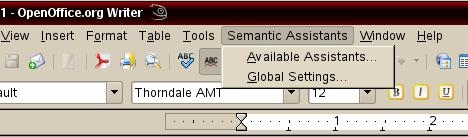
\includegraphics[width=0.7\textwidth]{pictures/oomenu.jpg}
\end{center}

In this menu, the user can inquire about available services, which are
selected based on the client (here \emph{Writer}) and the language
capabilities of the deployed NLP services (described in service
metadata, see Section~\ref{sec:owl}). The dynamically generated list
of available services is then presented to the user, together with a
brief description, in a separate window, as shown in
Figure~\ref{fig:oolist}. Note that the integration of a new service
does not require any changes on the client side---any new NLP service
created and deployed by a language engineer is dynamically discovered
through its OWL metadata maintained by the architecture and so becomes
immediately available to any connected client.
\begin{figure}[htb]
  \centering
  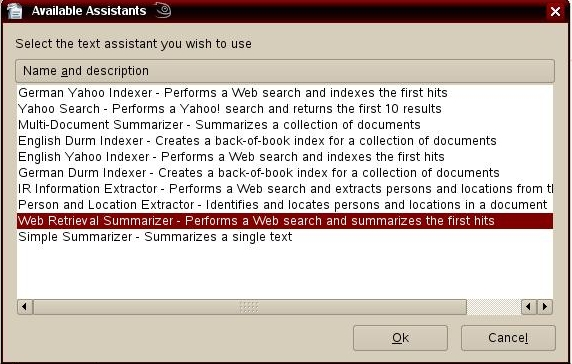
\includegraphics[width=0.5\textwidth]{pictures/oolist.jpg}
  \caption{List of available semantic assistants}
  \label{fig:oolist}
\end{figure}

The user can now select an assistant and execute it. In case the
service requires additional parameters, such as the length of a
summary to be generated, they are detected by our architecture through
the OWL-based service description and requested from the user through
an additional dialog window. An example, for the \emph{Web Retrieval
  Summarizer} assistant, is shown in Figure~\ref{fig:ooparams}.
\begin{figure}[htb]
  \centering
  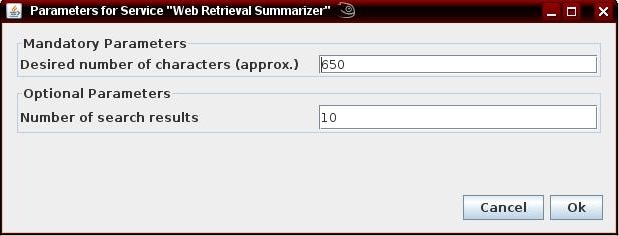
\includegraphics[width=0.5\textwidth]{pictures/ooparams.jpg}
  \caption{The parameters dialog, which appears when a Semantic
    Assistant requiring further input is invoked}
  \label{fig:ooparams}
\end{figure}
After the service is executed, the result is displayed in Writer depending on
the type of the server response: either as a new document, as annotations on
the existing document, or by opening an external viewer (e.g., a Web browser
for HTML documents).

\subsubsection{Side-Notes View}
The latest release of the OpenOffice.org Suite offer a new feature for text
annotation.  Depending on the annotation results received from GATE, the
Semantic Assistants Writer plug-in presents it in a sidenote manner (see
Figure~\ref{fig:sidenotes}).
\begin{figure}[htb]
  \centering
  %\vspace*{-9mm}
  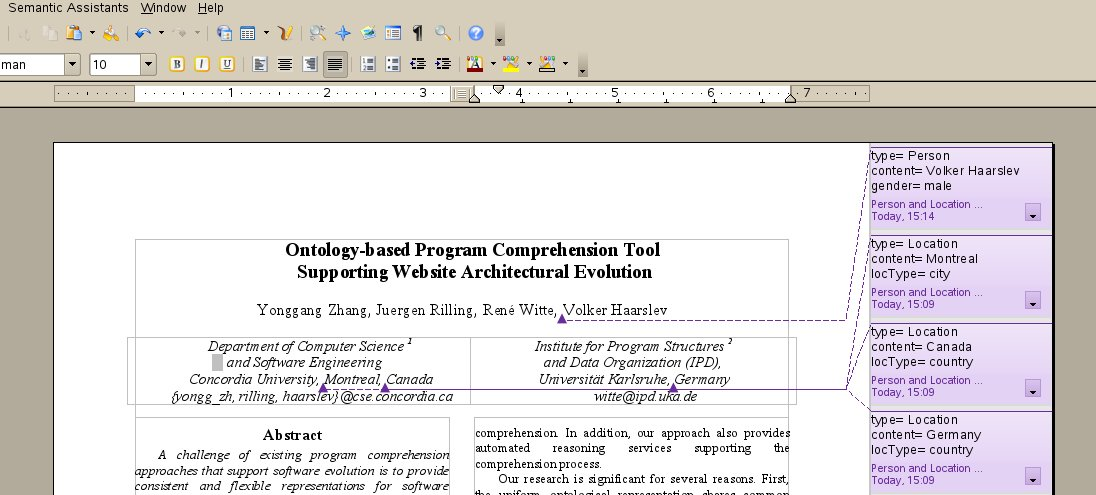
\includegraphics[width=0.8\textwidth]{pictures/sidenotes.jpg}
  \caption{Auto-Generated SideNotes Example}
  \label{fig:sidenotes}
  %\vspace*{-0.4cm}
\end{figure}

\subsubsection{New Document Creation}
\label{sec:doc-cre}
Creation of a new document comes handy when the output of an NLP service
corresponds to a complete document, or the result itself is indivisible. Some
examples are summarization or question-answering (see Figure~\ref{fig:oores}).

\begin{figure*}[htb]
  \centering
  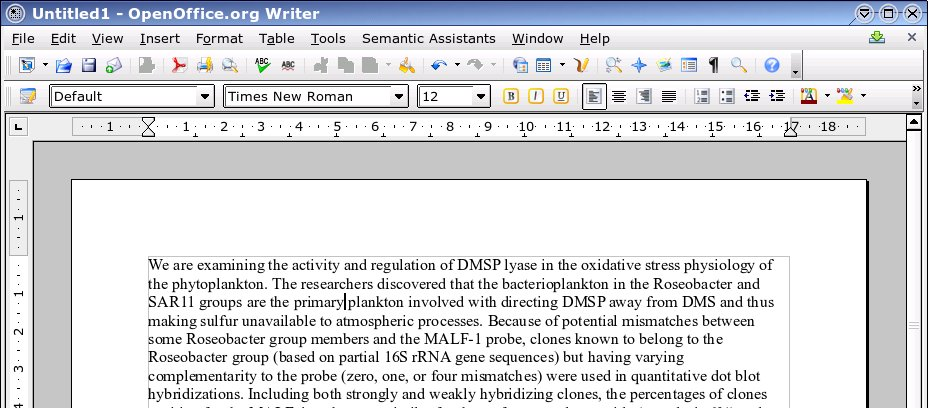
\includegraphics[width=0.8\textwidth]{pictures/ooresult_clip.jpg}
  \vspace*{-2mm}
  \caption{NLP services can also create a completely new document as a
  result (e.g., through summarization)}
  \label{fig:oores}
\end{figure*}

\subsubsection{Annotation Highlighting}
Besides text annotation, we offer the option for enabling/disabling annotation
highlighting for text that has been processed by GATE. This option can be
found under the Semantic Assistants menu in ``Global Settings.''  See
Figure~\ref{fig:highlight} for an example.

\subsubsection{Filter Empty Features}
This option found under the Semantic Assistants menu in ``Global Settings'' (shown
in Figure~\ref{fig:oosettings}) allows the ability to enable/disable filtering of
empty valued features in side-nodes. This can be useful to avoid cluttering or aid
debugging annotations respectively.

\subsubsection{Show Annotation Content}
This option in the ``Global Settings'' dialog can be used to include/exclude
the annotated content within the side-note. This can be used as an alternative
to annotation highlighting.

\begin{figure}
  \centering
  %\vspace*{-9mm}
  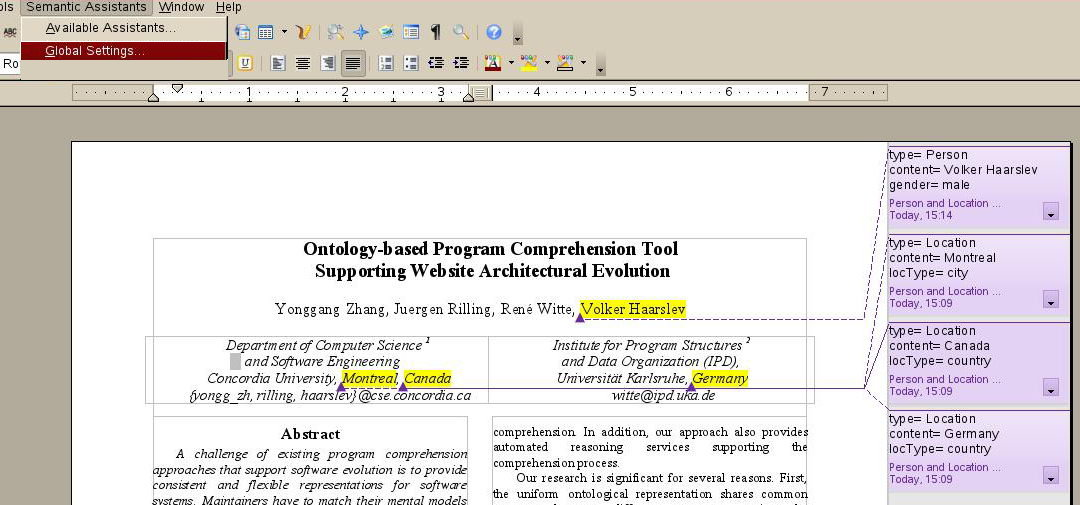
\includegraphics[width=0.8\textwidth]{pictures/highlighting.jpg}
  \caption{Highlighted Annotations Example}
  \label{fig:highlight}
  %\vspace*{0.5cm}
\end{figure}

\begin{figure}[htb]
\begin{center}
  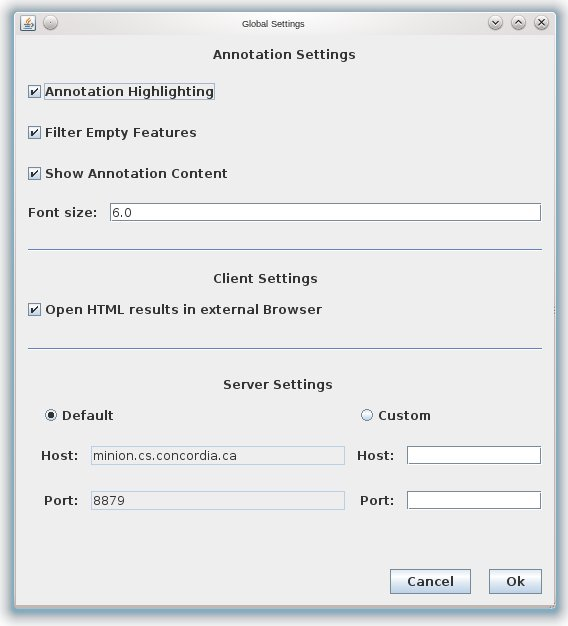
\includegraphics[width=0.5\textwidth]{pictures/oosettings.jpg}
  \caption{Configuration Dialog}
  \label{fig:oosettings}
\end{center}
\end{figure}

\subsubsection{Annotation Font Size}
As shown in Figure~\ref{fig:oosettings}, the font size of annotations can be changed
prior to invoking assistants. Due to the fixed width of side-notes, customizing the
size can ease readability of features.

\subsubsection{Browser Handling of HTML Results}
Instead of returning annotations, some pipelines produce HTML documents. The
``Open HTML results in external Browser'' option shown in Figure~\ref{fig:oosettings},
allows OpenOffice to invoke a local browser to display these results.

\subsubsection{Server Settings}
Another option found under the Semantic Assistants menu in ``Global
Settings.'' is \emph{Server Settings}.  There the user is able to specify the
Server information (Host and Port) of a local or distant server.

\subsection{Installation}
\label{subsec:oo-inst}
The OpenOffice.org plug-in can be found in
\url{SemanticAssistants/Clients/OpenOffice} and it is compatible with 
OpenOffice versions greater than 2.0.4. To use it, do the following:

\begin{enumerate}
  % TODO: what about the OO SDK installation? 
  % Is it needed for running the plug-in?

  \item Start OpenOffice.org Writer and ensure the right Java VM is
  used. Go to \emph{Tools $\rightarrow$ Options}. Under
  \emph{OpenOffice.org} you will find a \emph{Java} item. There, you
  can specify JREs. If it is not already there, add the currently used
  Java version.
  
  % should add screenshots for this
  \item Go to \emph{Tools $\rightarrow$ Extension Manager}. Click the
    \emph{Add$\ldots$} button on the bottom. Navigate to your local
    copy of the \sa\ architecture and then to
    \texttt{Clients/OpenOffice}. Select the file
    \texttt{SemassistOpenOfficePlugIn.oxt} and click \emph{Open}.

  \item Leave the dialog and open a new text document. You should have
    a new menu bar entry labeled \emph{Semantic Assistants}. Now you
    can run services on the current document (remember the server must
    be running to be able to query or execute language services).
\end{enumerate}


\subsection{Development Notes}
\label{sec:oo-spec}
In this section, we provide further technical details on our plug-in
for developers interesting in enhancing or modifying it.

\subsubsection{Compiling the Plug-in}
If you want to build the plugin yourself, follow these steps:
\begin{itemize}
  \item cd to the \url{Clients/OpenOffice} directory.

  \item Type \texttt{ant run}, or \texttt{ant run-gui}. Note that the
    client-side abstraction layer must have already been built and
    packaged. Both \texttt{ant run} and \texttt{ant run-gui} provide
    an UNO package named \url{SemassistOpenOfficePlugIn.oxt}. Both
    targets additionally copy it to \url{~/Documents/uno-components}.
    If \texttt{ant run-gui} is issued the OpenOffice.org
    \emph{Extension Manager} will pop up and prompt the user to
    install the extension.  If \texttt{ant run} is issued the above
    process is automated.  After the installation, OpenOffice Writer
    starts with the plug-in installed.

    \textbf{Note:} you can also manually add the plug-in from within
    OpenOffice (skip this step if you already used the \emph{run} or
    \emph{run-gui} target): Go to Tools, Extension Manager. Select
    \emph{My Extensions}, then click \emph{Add...} on the
    right. Choose the UNO package (available in
    \url{~/Documents/uno-components} if you used the \emph{deploy}
    target for ant).
\end{itemize}

\subsubsection{OpenOffice.org Plug-in Specifics}
Every plug-in has to include a \emph{description.xml} that describes the 
package's meta details like publisher, license, download url and version dependencies.
See \href{http://wiki.services.openoffice.org/wiki/Documentation/DevGuide/Extensions/Description_of_XML_Elements}{OpenOffice Developer's Guide}
for a list of available elements. The plug-in package also includes a
\emph{META-INF} directory, which contains a file called
\emph{manifest.xml}. This XML file lists the elements that come with
this plug-in;  The concrete manifest file for our plug-in is listed in
Figure~\ref{list:manifest}.  We can see that it defines three
\emph{file-entry} elements specifying the type and location of the
following files:
\begin{figure}[tb]
\centering
\begin{lstlisting}[language=XML,numbers=left,xleftmargin=8mm,columns=flexible]
<?xml version="1.0" encoding="UTF-8"?> 
<!DOCTYPE manifest:manifest PUBLIC 
"-//OpenOffice.org//DTD Manifest 1.0//EN" "Manifest.dtd"> 
<manifest:manifest 
 xmlns:manifest="http://openoffice.org/2001/manifest"> 
  <manifest:file-entry 
     manifest:media-type=
        "application/vnd.sun.star.configuration-data" 
     manifest:full-path="Addons.xcu"/> 
  <manifest:file-entry 
     manifest:media-type=
        "application/vnd.sun.star.configuration-data" 
     manifest:full-path="ProtocolHandler.xcu"/> 
  <manifest:file-entry 
     manifest:media-type=
        "application/vnd.sun.star.uno-component;type=Java" 
     manifest:full-path=
        "ProtocolHandlerAddon_java.uno.jar"/>
   <!-- Add any other plug-in required jar files here. -->
</manifest:manifest> 
\end{lstlisting}
\caption{The \emph{manifest.xml} file for our plug-in}
\label{list:manifest}
\end{figure}


\begin{description}
\item[\emph{Addons.xcu}.] This XML file defines how the plug-in should
  be integrated with OpenOffice.org. In our case, it contains a menu
  definition, specifying that the menu should only appear in the
  \emph{Writer} application. For each menu item, we specify which
  messages should be broadcast throughout the OpenOffice.org runtime
  system when the menu item is activated.
\item[\emph{ProtocolHandler.xcu}. ] This XML file specifies that the
  messages defined in \emph{Addons.xcu} should be handled by an object
  of a certain class. This class is provided in the Java archive and
  must adhere to a certain interface. 
\item[\emph{ProtocolHandlerAddon\_ java.uno.jar}.] This Java archive
  contains the actual functionality of the plug-in. It holds classes
  responsible for receiving the messages generated by the menu items,
  as well as classes responsible for the interaction with the
  client-side abstraction layer.
\end{description}


\subsubsection{Implementation Details}
A useful class called \url{UNOUtils} found in the \url{package
  info.semanticsoftware.semassist.client.openoffice.utils} contains most of
the OO-Writer feature implementations.  More specifically, the three methods in
Figure~\ref{list:ssb} implement a major part of the above described features
(Side-Notes, Highlighting and New Document Creation).

\begin{figure}
\centering
\begin{lstlisting}[language=Java,numbers=left,xleftmargin=8mm,columns=flexible]

private static XComponent CreateNewDocument( XDesktop xDesktop, 
					     String sDocumentType )
{
	...
}

private static void AnnotateField( Annotation annotation )
{
	...
	// Use the text document's factory to create an Annotation text field
	XTextField xAnnotation = (XTextField) UnoRuntime.queryInterface(
		XTextField.class, mxDocFactory.createInstance(
		"com.sun.star.text.TextField.Annotation" ) );
	
	// get the properties of the field
	XPropertySet xPropertySet = (XPropertySet) UnoRuntime.queryInterface( 
						XPropertySet.class, xAnnotation
);
	
	...
	
	// Highlight annotated field
        HighlightField();
}

private static void HighlightField()
{
....

}
\end{lstlisting}
\caption{Core methods implementing the OpenOffice Writer plug-in features are
  part of the \texttt{UNOUtils} class}
\label{list:ssb}
\end{figure}

%More details on how to compile and debug an OpenOffice plug-in can be found in Section~\ref{sec:debug}.
 
\subsubsection{Configure the OpenOffice Writer to Run in Debug Mode}
This Section describes how to configure the JAVA VM in OpenOffice Writer to accept incoming connection for a debugger.

\begin{enumerate}
  \item Open OpenOffice Writer
  \item Go to Tools, Options. Under \emph{OpenOffice.org}, there is a \emph{Java} item. Select it and then Click on the 
        \emph{Parameter} button. There the parameters when running the JAVA VM are set.
  \item To run in debug mode \emph{Assign} the following 2 parameters:
  \begin{itemize}
    \item \textbf{-X debug}
    \item \textbf{-Xrunjdwp:transport=dt\_socket,server=y,suspend=n,address=7081}
  \end{itemize}
  \item \textbf{Note: The} \emph{address=7081} \textbf{should be the consistent with the port set within the debugger}
  \item  Now OO Writer is ready to accept connections from the debugger
\end{enumerate} 


\section{Eclipse Plug-in}
Eclipse is not a single monolithic program, but rather a small kernel containing
a plug-in loader surrounded by hundreds of plug-ins. The behavior of each
plug-in in this architecture is stored in its code, and its dependencies and
services are declared in the plug-in's manifest file. On each Eclipse startup,
the plug-in loader scans all the available manifest files in the Eclipse
exclusive plug-in folder and then builds a structure containing this
information.

We used this characteristic of Eclipse architecture to integrate our Semantic
Assistants architecture into the Eclipse environment in form of a plug-in, in
order to offer various Natural Language Processing services. The Semantic
Assistants Eclipse plug-in is basically a Java archive (JAR) file that ships
with its own specific content and a description file to introduce itself to the
Eclipse plug-in loader. 

\subsection{Features}
Once the Semantic Assistants plug-in is installed, it creates a new menu entry
in the Eclipse menu toolbar. A user can inquire about the available services
from the ``Available Assistants'' item and modify the connection settings to the
Semantic Assistants server by selecting the second item.
\begin{figure}[htb]
\begin{center}
  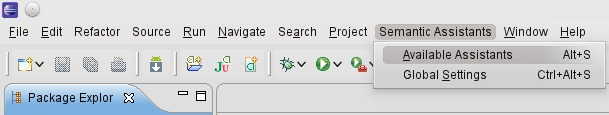
\includegraphics[width=1.0\textwidth]{pictures/eclipse_menu.jpg}
  \caption{Semantic Assistant Menu in Eclipse}
  \label{fig:eclipse_menu}
\end{center}
\end{figure}
\subsubsection{Available Assistants}
Selecting the ``Available Assistants'' item from Semantic Assistants menu will
open a file selection dialog. The file selection dialog allows the user to
select the desired files, folders and even complete projects to send to the
server as inputs to an NLP service. For more convenience, you can type an arbitrary extension like ``java'' or ``xml'', in the ``File Format'' field to filter to file tree view. 

\begin{figure}[htb]
\begin{center}
  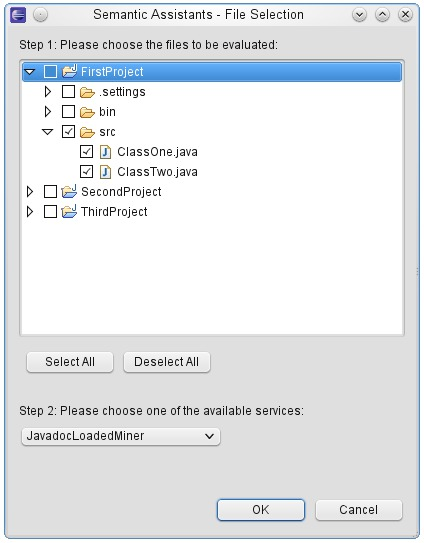
\includegraphics[width=0.5\textwidth]{pictures/eclipse_fileSelection.jpg}
  \caption{File Selection Dialog}
  \label{fig:eclipse_fileSelection}
\end{center}
\end{figure}

This dialog also lets the user to select an NLP service from a dynamically
generated list of services. This list is generated dynamically by selecting the
available services based on the client and the language capabilities of the
deployed NLP services. The server location where the service information are read from is presented just above the list as depicted in Fig \ref{fig:eclipse_services}. Note that the integration of a new service does not
require any changes on the client side - any new NLP service created and
deployed by a language engineer is dynamically discovered through its OWL
metadata maintained by the architecture and so becomes immediately available to
any connected client.

\begin{figure}[htb]
\label{fig:eclipse_services}
\begin{center}
  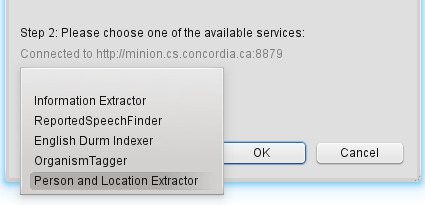
\includegraphics[width=0.5\textwidth]{pictures/eclipse_services.jpg}
  \caption{A List of Available NLP Services}
  \label{fig:eclipse_services}
\end{center}
\end{figure}

Upon selecting the resource files and the desired service, the user can execute
the selected service on the checked files in the tree. Consequently, the user will be informed about the status of the execution in the ``Semantic Assistant Status'' view. A successful execution of the selected NLP service, will let the user know on how to view the results. If the service execution fails, a description of the occurred error will be shown to the user and invocation will be aborted.

Now, let's look at how different types of outputs are handled in the plug-in:

\paragraph{Annotations.}
Annotations retrieved from a successful service invocation are being shown to the user in an
Eclipse view part called ``Semantic Assistants'' view. In the mentioned view, a
table will be dynamically generated that contains
all the parsed annotation instances. In Figure~\ref{fig:eclipse_saView} the
result of an execution of the ``Person and Location Extractor'' service on two
sample classes is shown.
\begin{figure}[htb]
\begin{center}
  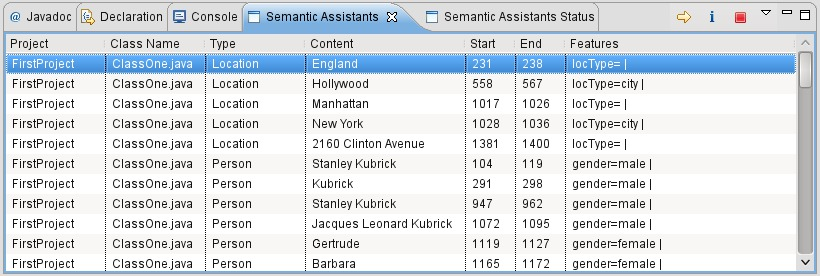
\includegraphics[width=1\textwidth]{pictures/eclipse_saView.jpg}
  \caption{Semantic Assistants View}
  \label{fig:eclipse_saView}
\end{center}
\end{figure}

This table can be sorted by different criteria through clicking on each column
title. Additionally, by double-clicking on each row in the table, the selected
annotation will appear with a graphical representation attached to the
corresponding resource. For instance, in Figure~\ref{fig:eclipse_annotation} the
JavadocMiner service has been invoked on a Java source code file. Some of the
annotations returned by the server bear a \emph{lineNumber} feature, which
attaches an annotation instance to a specific line in the java source file. Upon
double-clicking on the annotation instance in the Semantic Assistant view, the
corresponding resource - here, a .java file - will be opened in an editor and an
Eclipse warning marker will appear next to the line defined by the annotation
\emph{lineNumber} feature.

\begin{figure}[htb]
\begin{center}
  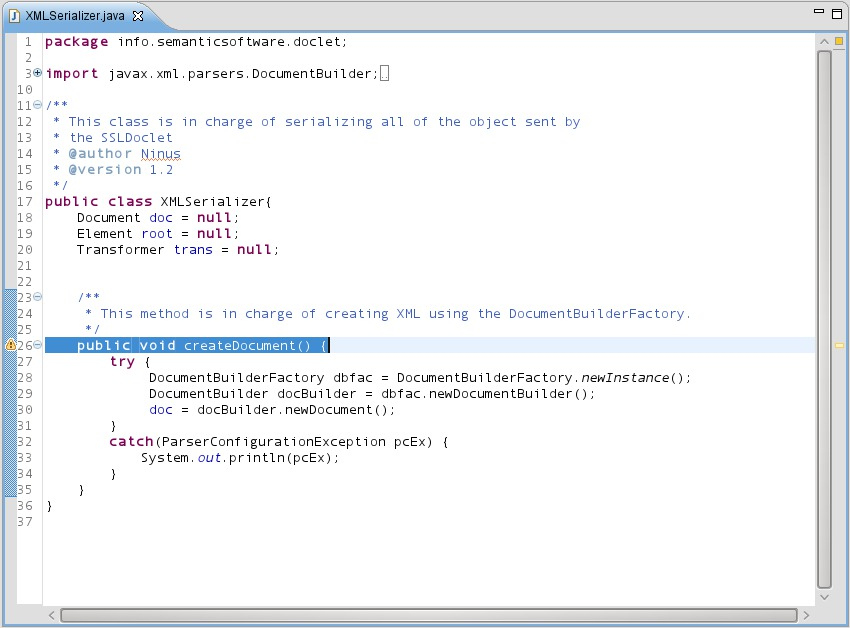
\includegraphics[width=1\textwidth]{pictures/eclipse_annotation.jpg}
  \caption{A Semantic Annotation}
  \label{fig:eclipse_annotation}
\end{center}
\end{figure}

\paragraph{Boundless Annotations.}
Boundless Annotations are a special kind of Annotations that adhere to a whole document and thus have no start and end offset. The plug-in parses the annotation results, and then inserts the content of the annotations in a new document and opens it in a new editor inside the Eclipse environment.

\paragraph{Documents.}
Documents received from the server response carry a URL property where defines where they are located. The plug-in retrieves the URLs and inserts them into a new document that opens up in a new editor inside the Eclipse environment.

\paragraph{Files.}
When a file output type is received by the plug-in, it will try to open it up in a web browser. In Eclipse, users can configure whether they want to open URLs in the Eclipse built-in web browser or any other ones in the file system. Whichever defined as the default behavior in Eclipse by the user, will be used by the plug-in to present the result file to the user. In this case, a log message will be shown to the user in the ``Semantic Assistants Status'' view to inform the user that the file is opened in his browser.

\subsubsection{Global Settings}
The second option found under the Semantic Assistants menu is the ``Global
Settings'' item. By clicking on this menu item, a dialog as depicted in Figure \ref{fig:eclipse_settings} is shown to the user that lets him choose a preferred server from a list of pre-defined values or add a custom server to the settings file. The values are provided in the Semantic Assistants global preference file described in \ref{sec:pref_management}. If the preference file gets accidentally deleted, a default preference file will be created by the plug-in but the eclipse-specific settings will be lost.
\begin{figure}[htb]
\begin{center}
  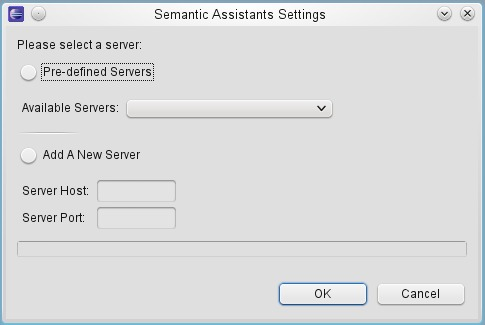
\includegraphics[width=0.6\textwidth]{pictures/eclipse_settings.jpg}
  \caption{Semantic Assistants Server Settings Dialog}
  \label{fig:eclipse_settings}
\end{center}
\end{figure}

\subsection{Installation}
\label{subsec:eclipse_install}
You can install the Semantic Assistants plug-in via the Eclipse software installer. To do so, first you have to add the Semantic Assistants software repository to your Eclipse list of software sites. In addition to installing the plug-in, adding the repository lets the Eclipse update manager to check for plug-in updates once available. Please carefully follow the steps listed below to install the Eclipse plug-in and refer to section \ref{trouble:eclipse_install} for installation troubleshooting.

\begin{enumerate}
  \item Select Help $\rightarrow$ Install New Software to open the Eclipse software installer.
  \item Press the ``Add'' button in the dialog, to add the Semantic Assistants repository.
  \item In the new dialog depicted in Fig \ref{fig:eclipse_install}, type ``\texttt{Semantic Assistants}'' and\\ ``\texttt{http://sa-eclipse.semanticsoftware.info}'' in ``Name'' and ``Location'' fields, respectively, and press ``OK''.
  \item The Semantic Assistants repository should now be added to your Eclipse list of software sites as seen in Fig \ref{fig:eclipse_install2}. From the loaded softwares, check the Eclipse plug-in and press ``Next''.
  \item Simply, follow the installation steps and let the installer restart the Eclipse application.
  \item The Eclipse plug-in loader will automatically load the plug-in for you. If the plug-in is installed
successfully, you should be able to see the Semantic Assistants menu added to
you toolbar.
\end{enumerate}

\begin{figure}[htb]
\begin{center}
  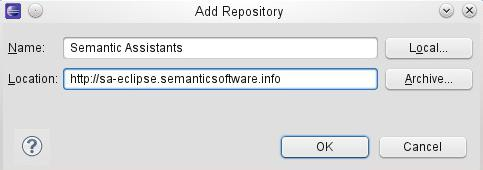
\includegraphics[width=0.6\textwidth]{pictures/eclipse_install.jpg}
  \caption{Adding Semantic Assistants Repository to Eclipse List of Software Sites}
  \label{fig:eclipse_install}
\end{center}
\end{figure}

\begin{figure}[htb]
\begin{center}
  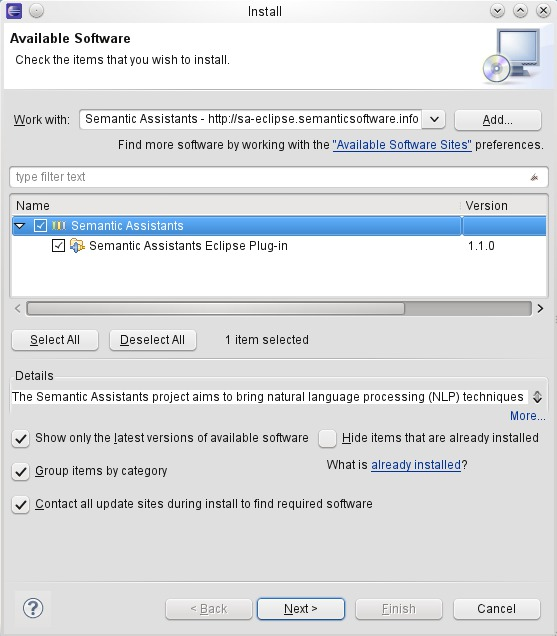
\includegraphics[width=0.6\textwidth]{pictures/eclipse_install2.jpg}
  \caption{Eclipse Software Installer Dialog}
  \label{fig:eclipse_install2}
\end{center}
\end{figure}

\subsection{Updating The Plug-in}
\begin{enumerate}
  \item Select Help $\rightarrow$ Check for Updates to open the Eclipse update manager.
  \item If there are any updates available for the Semantic Assistants plug-in, it will appear the in the update manager dialog as shown in Fig \ref{fig:eclipse_update}.
  \item Check the Semantic Assistants Eclipse plug-in from the list and press ``Next''.
  \item Follow the wizard steps and let the update manager restart your Eclipse for the updates to take place.
\end{enumerate}

\begin{figure}[htb]
\begin{center}
  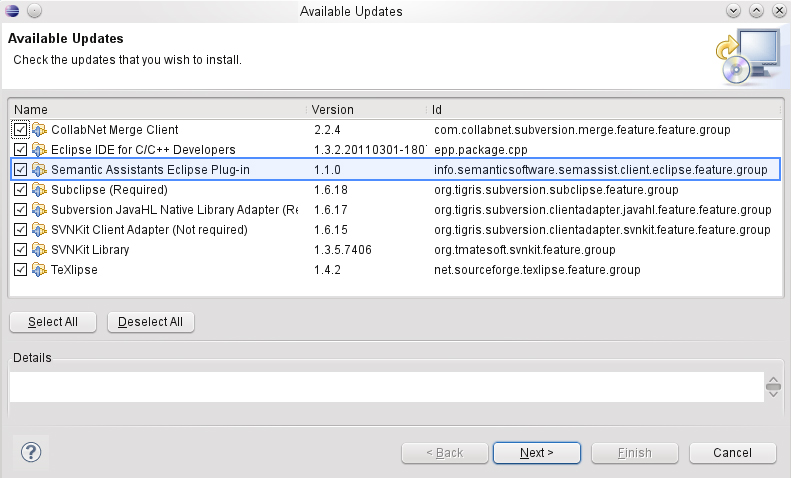
\includegraphics[width=1.0\textwidth]{pictures/eclipse_update.jpg}
  \caption{Updatin the Plug-in via Eclipse Update Manager}
  \label{fig:eclipse_update}
\end{center}
\end{figure}

\subsection{Development Notes}
\label{subsec:eclipse.development}
In this section, we provide further technical details on our plug-in for
developers interesting in enhancing or modifying it.

\subsubsection{Plug-in Source Directory Structure}
The Semantic Assistants plug-in uses Model-View-Controller pattern for its
implementation. Thus, most of the source code files are divided into different
packages related to their responsibilities. When you browse to
\url{src/info/semanticsoftware/semassist/client/eclipse/} folder, you see the
following structure:
\begin{enumerate}
\item\url{dialogs}: This folder contains the dialogs that are shown to the user
for interactions e.g. file selection. The classes inside this folder are the
codes for graphical user interfaces.
\item\url{handlers}: This folder contains the classes which play the controller
role in MVC pattern. Examples of these classes are dialog handlers and service
invocation jobs.
\item\url{model}: This folder contains the classes that provide data for
graphical user interfaces. These models are consumed by classes inside
\texttt{views} package.
\item\url{utils}: This folder contains utility classes e.g. logging feature.
\item\url{views}: This folder contains the source codes for Semantic Assistants
view parts. These are again graphical user interfaces but packaged differently
from dialogs.
\end{enumerate}

There is also another file called \url{Activator.java} in the source directory.
It is the main class of the plug-in that will be loaded initially and control
the plug-in's life cycle.

\subsubsection{Modifying the Plug-in}
If you want to modify the plug-in behavior or enhance it, follow these steps:
\begin{enumerate}
\item Open the Eclipse application.
\item Select File $\rightarrow$ New  $\rightarrow$ Project and under the
``Plug-in Development'' category select the ``Plug-in Project''.
\item A new plug-in project wizard will open up. Keep the EclipsePlugin name for
the project. Just below the project name there is a checkbox reading ``Use
Default Location''. Uncheck it and browse to the EclipsePlugin folder inside
where you've stored the Semantic Assistants folder.
\item Leave the other options untouched and press Finish.
\end{enumerate}

\begin{figure}[htb]
\begin{center}
  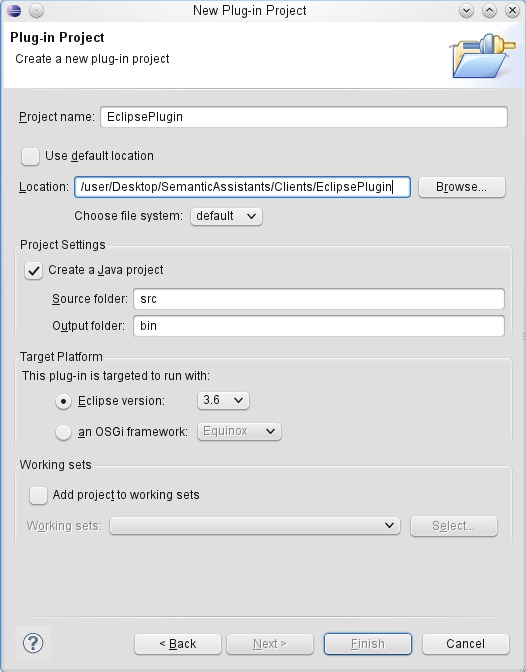
\includegraphics[width=0.5\textwidth]{pictures/eclipse_project_wizard.jpg}
  \caption{Eclipse New Plug-in Project Wizard}
  \label{fig:eclipse_project_wizard}
\end{center}
\end{figure}

\textbf{Note:} Remember you should manually copy the CSAL.jar file into you the
project's \texttt{lib} folder because it is a part of the project's dependency
and is defined in the classpath.

When the project is loaded in your workspace, feel free to play around. Browse
the source directory and add your development codes. To run your code, right
click on \texttt{plugin.xml} file and select Run As $\rightarrow$ Eclipse
Application.


\section{Extension for Mozilla Firefox and Mozilla Thunderbird} 

The Mozilla extension allows users to use Semantic Assistants in Mozilla Firefox and Mozilla Thunderbird and to leverage the \sa architecture within those applications. It is built on the extension platform that shared by Mozilla Firefox and Mozilla Thunderbird. Hence, it is a single extension that is compatible with both applications. The Mozilla extension aims to take the capabilities provided by Semantic Assistants and integrate them within the workflow of web browsing and of email reading and management. 

\subsection{Features}
\label{subsec:mozilla_features}

\subsubsection{User Interface Elements}
When the \sa Mozilla extension is installed, some new UI elements are added to the interface of the application. Firstly, a new ``Semantic Assistants" menu is added on the menu bar. Secondly, a new toolbar button is added to the primary toolbar of the application. (This toolbar button may be removed or relocated using Firefox/Thunderbird's built-in customization capabilities.) The toolbar button is actually a ``menu button," i.e., the left part is a button, and the right part opens a menu when clicked. Thirdly, a menu item is added to the contextual (right-click) menu of the principal content area of the application, that is, the browsing area in Firefox and the message body pane in Thunderbird. Lastly, a sidebar, which can be opened and closed, is added to the main window of the application. 

\paragraph{The ``Semantic Assistants" menu.} The ``Semantic Assistants" menu is 
located on the menu bar and opens a menu with the following three menu items: 
\begin{itemize} 
  \item Available Assistants... 
  \item Semantic Assistants Sidebar 
  \item Global Settings... 
\end{itemize} 

The ``Semantic Assistants" menu is shown in Figure~\ref{fig:mozilla_features_toolbar_menu_button}. 

\begin{figure}[htb]
  \centering
  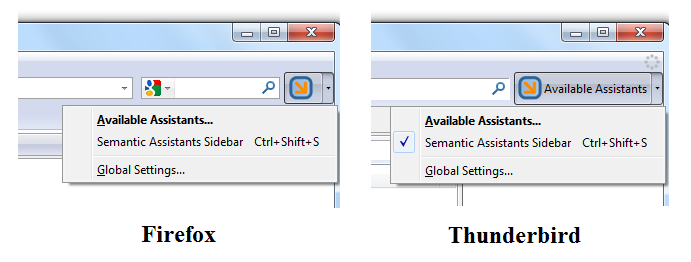
\includegraphics[width=0.8\textwidth]{pictures/mozilla_features_toolbar_menu_button.png}
  \caption{The toolbar menu button in Firefox and Thunderbird}
  \label{fig:mozilla_features_toolbar_menu_button}
\end{figure}

\paragraph{The ``Available Assistants" toolbar menu button.} The ``Available Assistants" menu button is located on the toolbar. The left side is a button and executes the ``Available Assistants" command (further elaborated later). Clicking the right side opens a menu that is identical to the ``Semantic Assistants" menu. 

\paragraph{The ``Available Assistants..." contextual menu item.} The ``Available Assistants" menu item appears on the contextual (right-click) menu of the main browsing area/page content area in Firefox and in the message body area in Thunderbird. Like the toolbar button, it also invokes the ``Available Assistants" command. 

\paragraph{The ``Semantic Assistants Sidebar".} The ``Semantic Assistants Sidebar" appears on the left side of the main window in Firefox and on the right side of the main window in Thunderbird. (The discrepancy is explained as follows. Firefox has built-in support for adding sidebars, and these appear on the left side of the main browsing window. Thunderbird, on the other hand, has no sidebars. Furthermore, the main inbox tab in Thunderbird already has a folder pane on the left side of the window. Hence, a custom sidebar was added, and it was placed on the right side of the main window.) 

The ``Semantic Assistants Sidebar" displays the results obtained from a service invocation to a Semantic Assistant. The following button in the Sidebar operate on the results: 
\begin{itemize} 
  \item \emph{Expand all}: Expands nodes of the results tree by one level.
  \item \emph{Collapse all}: Collapses all nodes of the results tree.
  \item \emph{Underline all}: Underlines all results in the tree in the page/message.
  \item \emph{Underline none}: Clears all the underlining in the page/message.
  \item \emph{Find previous underlined item}: Selects (highlights) the previous underlined text in the page/message.
  \item \emph{Find next underlined item}: Selects (highlights) the next underlined text in the page/message.
\end{itemize} 
The ``Semantic Assistants Sidebar" can be opened using the following ways: 
\begin{itemize} 
  \item \emph{Semantic Assistants} menu $\rightarrow$ \emph{Semantic Assistants Sidebar}
  \item \emph{Available Assistants} toolbar button menu $\rightarrow$ \emph{Semantic Assistants Sidebar}
  \item (in Firefox) \emph{View} menu $\rightarrow$ \emph{Sidebar} $\rightarrow$ \emph{Semantic Assistants Sidebar}
  \item (in Thunderbird) \emph{View} menu $\rightarrow$ \emph{Layout} $\rightarrow$ \emph{Semantic Assistants Sidebar}
  \item the keyboard shortcut \emph{Ctrl Shift S}
\end{itemize} 

The ``Semantic Assistants Sidebar" dialog is shown in Figure~\ref{fig:mozilla_features_sidebar}. 

\begin{figure}[htb]
  \centering
  % \includegraphics[width=0.8\textwidth]
  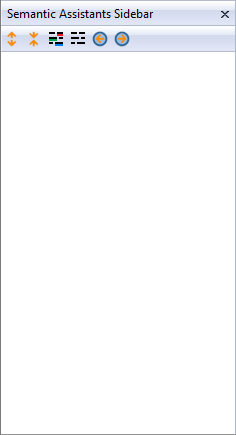
\includegraphics[totalheight=0.5\textheight]{pictures/mozilla_features_sidebar.png}
  \caption{The ``Semantic Assistants Sidebar" in Firefox and Thunderbird}
  \label{fig:mozilla_features_sidebar}
\end{figure}

\paragraph{The ``Global Settings" dialog.} The ``Global Settings" dialog allows the user to configure certain settings for the extension. These settings include:
\begin{itemize} 
  \item \emph{Server settings}: The user may choose to use the default defined server or to specify a custom server address. 
  \item \emph{Script settings}: The processing of the results is handled by a script run in Firefox/Thunderbird. If there are a lot of results or the page/message is long, the script may run for a long time. Firefox/Thunderbird has the built-in capability to prompt the user when a script has run for a given amount of time. By default, this amount of time is 20 seconds. The user may change this period if desired. Setting this setting to 0 signifies that the script will run forever. (Doing so, however, is not recommended, as the script may run for a very long time, and the only way to cancel would be to kill the whole application.)
\end{itemize} 
The ``Global Settings" dialog can be opened using the following ways: 
\begin{itemize} 
  \item \emph{Semantic Assistants} menu $\rightarrow$ \emph{Global Settings...}
  \item \emph{Available Assistants} toolbar button menu $\rightarrow$ \emph{Global Settings...}
\end{itemize} 

The ``Global Settings" dialog is shown in Figure~\ref{fig:mozilla_features_global_settings}. 

\begin{figure}[htb]
  \centering
  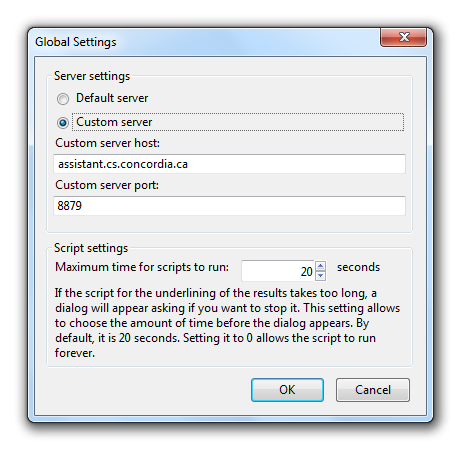
\includegraphics[width=0.8\textwidth]{pictures/mozilla_features_global_settings.png}
  \caption{The ``Global Settings" dialog in Firefox and Thunderbird}
  \label{fig:mozilla_features_global_settings}
\end{figure}

\subsubsection{Invoking a Semantic Assistant}
When the ``Available Assistants" command is invoked (either using the menu item in the ``Semantic Assistants" menu or in the menu of the toolbar button), a dialog entitled ``Available Semantic Assistants Services" appears (shown in Figure~\ref{fig:mozilla_features_available_assistants_dialog}), listing all available services from the server along with descriptions of each service. Upon the selection of a service, the extension sends the user-selected text in the page/message or, if text no selection was made, the whole text content of the page/message.

\begin{figure}[htb]
  \centering
  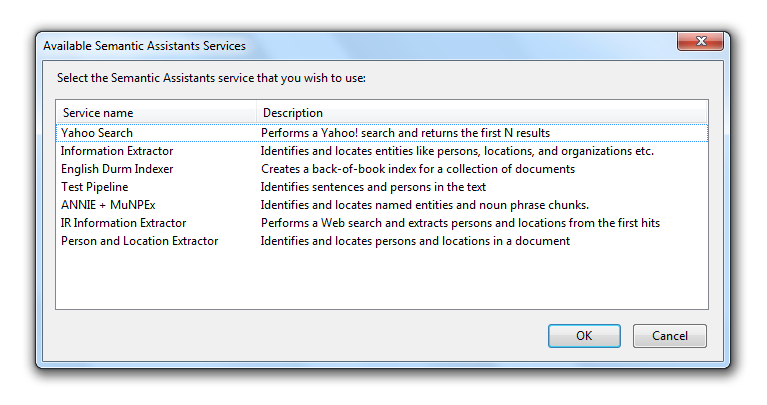
\includegraphics[width=1\textwidth]{pictures/mozilla_features_available_assistants_dialog.png}
  \caption{The ``Available Semantic Assistants Services" dialog in Firefox and Thunderbird}
  \label{fig:mozilla_features_available_assistants_dialog}
\end{figure}

When the results are returned by the server, two things happen. Firstly, the results are underlined in the page/message directly in the browsing area/message content area. Secondly, the ``Semantic Assistants Sidebar" is opened if it is not already so and displays the results. 

\subsubsection{Viewing the Results}
The results from the service invocation are underlined directly in the content of the page/message. The underlining is color-coded by annotation type to allow for better visual distinction. 

The results are also displayed in the ``Semantic Assistants Sidebar" in a tree format, grouped by annotation type, then by occurrences of a same word/phrase. 

The controls/buttons in the ``Semantic Assistants Sidebar" (mentioned previously in the ``User Interface Elements" section) can be used to manipulate the results tree, to underline all or no results and to go to the previous/next underlined result in the page/message.

Clicking on a node in the results tree will underline in the page/message the result or results represented by the node and all children of the node. For instance, if a leaf node of the tree is clicked in the Sidebar, the one result represented by that node is underlined. If an inner node of the tree is clicked in the Sidebar, then all the results represented by that node and all its child nodes are underlined. The ``Find previous underlined item" and ``Find next underlined item" buttons in the Sidebar will navigate only the currently underlined results. All put together, this allows to display precise subsets of the results, and to navigate through the occurrences of these results. 

The display of results within Firefox and Thunderbird is shown in Figure~\ref{fig:mozilla_features_firefox_window} and Figure~\ref{fig:mozilla_features_thunderbird_window_message_tab}.

\begin{figure}[htb]
  \centering
  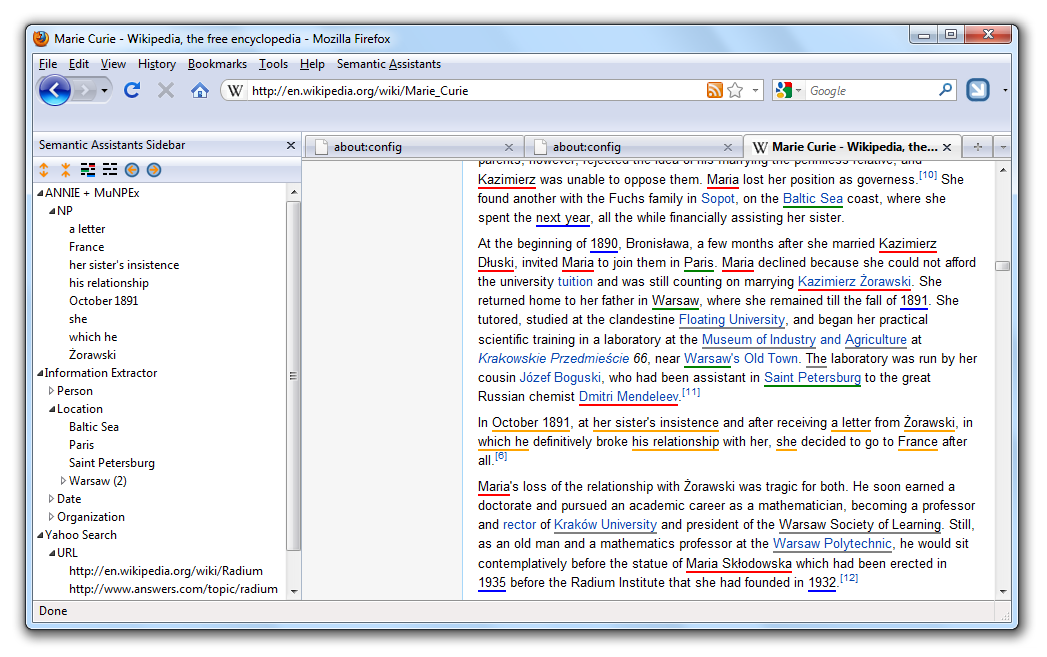
\includegraphics[width=0.95\textwidth]{pictures/mozilla_features_firefox_window.png}
  \caption{Results from a service invocation in Firefox}
  \label{fig:mozilla_features_firefox_window}
\end{figure}

\begin{figure}[htb]
  \centering
  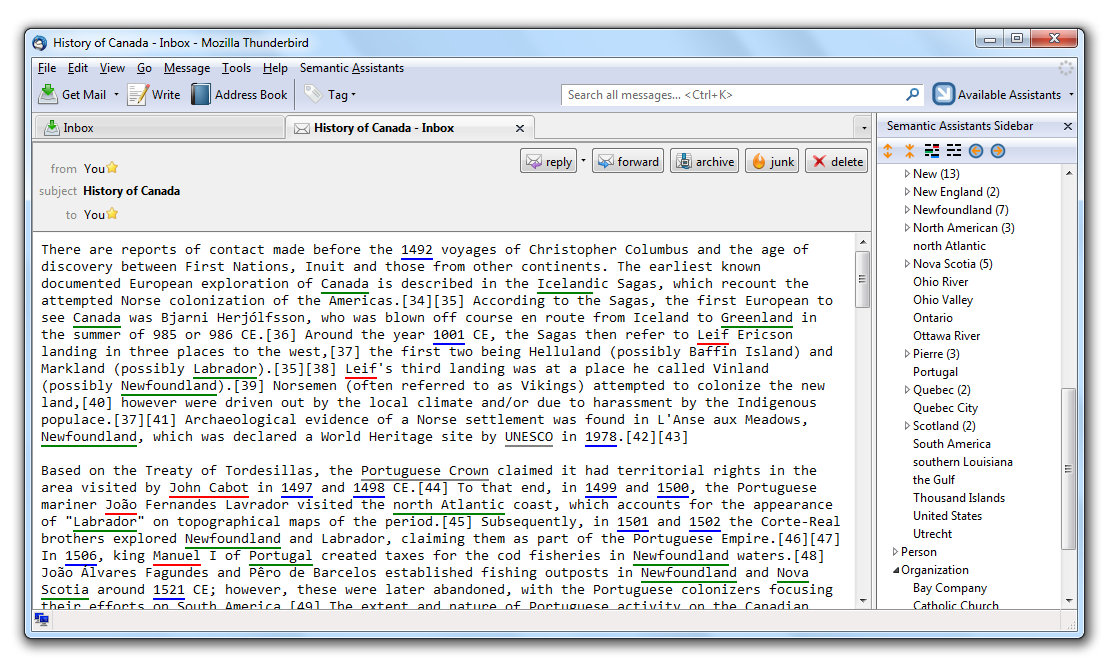
\includegraphics[width=0.95\textwidth]{pictures/mozilla_features_thunderbird_window_message_tab.png}
  \caption{Results from a service invocation in Thunderbird}
  \label{fig:mozilla_features_thunderbird_window_message_tab}
\end{figure}

\subsection{Installation}
\label{subsec:mozilla_installation}
The Mozilla extension comes in the form of a file with a .xpi extension. The .xpi file is installed in the standard manner in which extensions are installed in Mozilla Firefox and Mozilla Thunderbird. 

\subsubsection{Additional Notes about Prerequisites}
In addition to the basic prerequisites (refer to Chapter~\ref{chap:inst}), the following considerations should be noted: 
\begin{itemize}
  \item The Java runtime environment \emph{must} be the official Java Development Kit from Oracle (formerly from Sun). In certain Linux installations, OpenJDK is installed by default. This will not work for the Mozilla extension. (A ``java is not defined" error will occur.)
\end{itemize}

\subsubsection{Installation in Mozilla Firefox}
There are two methods to install the .xpi file in Firefox. The first method is to drag and drop the .xpi file into Firefox.
\begin{enumerate}
  \item Drag and drop the .xpi file into the main browsing area of the Firefox window.
  \item A dialog window entitled "Software Installation" appears. Click the ``Install Now'' button in the dialog.
  \item Restart Firefox.
\end{enumerate}
An alternate method is to use the file picker in Firefox.
\begin{enumerate}
  \item Select \emph{File $\rightarrow$ Open File...}.
  \item Navigate to the location of the .xpi file and choose it.
  \item A dialog window entitled "Software Installation" appears. Click the ``Install Now'' button in the dialog.
  \item Restart Firefox.
\end{enumerate}

\subsubsection{Installation in Mozilla Thunderbird 3.1.x and earlier}
Here is how to install the .xpi file in Thunderbird version 3.1.x and earlier. 
\begin{enumerate}
  \item Select \emph{Tools $\rightarrow$ Add-ons}.
  \item The Add-ons dialog opens. In the ``Extensions" section, at the bottom left, there is a button ``Install...". Click this button.
  \item Navigate to the location of the .xpi file and choose it.
  \item A dialog window entitled "Software Installation" appears. Click the ``Install Now'' button in the dialog.
  \item Restart Thunderbird.
\end{enumerate}

\subsubsection{Installation in Mozilla Thunderbird 5.0 and later}
Here is how to install the .xpi file in Thunderbird version 5.0 and later. 
\begin{enumerate}
  \item Select \emph{Tools $\rightarrow$ Add-ons}.
  \item The Add-on Manager opens. Near the top right, there is a button ``Tools for all add-ons" with a cog icon. Click this button.
  \item Click the ``Install Add-on from File" menu item.
  \item Navigate to the location of the .xpi file and choose it.
  \item A dialog window entitled "Software Installation" appears. Click the ``Install Now'' button in the dialog.
  \item Restart Thunderbird.
\end{enumerate}

If the installation succeeded, after the application restarts, the ``Semantic Assistants" menu in the menu bar should be visible, and the ``Available Assistants" toolbar button should be added to the toolbar. (For a full list of the UI elements of the extension, refer to section ~\ref{subsec:mozilla_features}.)

\subsection{Development Notes}
\label{subsec:mozilla_development}
This section details the layout of files in the extension, the overall architecture of the extension, and some specifics relating to Mozilla extension development. 

\subsubsection{A Brief Explanation of Mozilla Extensions}
An extension for the Mozilla platform is initially packaged in a .xpi file, which is simply a .zip file with the ``.xpi" file extension. Once the extension is ``installed" by the user, the contents of the .xpi file is extracted and placed in a newly created folder located in the ``extensions" folder within the Firefox/Thunderbird user profile folder. 

After the application restarts, the extension is loaded into memory, the installation of the extension to that specific user profile is complete.  

The Firefox/Thunderbird user profile folder is located at: 
\begin{itemize}
  \item Firefox \begin{itemize}
    \item On Windows XP: C:\textbackslash Documents and Settings\textbackslash WINDOWS\_ACCOUNT\_USER\_NAME \textbackslash Application Data\textbackslash Mozilla\textbackslash Firefox\textbackslash Profiles\textbackslash PROFILE\_FOLDER\_NAME
    \item On Windows Vista, 7: C:\textbackslash Users\textbackslash WINDOWS\_ACCOUNT\_USER\_NAME\textbackslash AppData\textbackslash Roaming \textbackslash Mozilla\textbackslash Firefox\textbackslash Profiles\textbackslash PROFILE\_FOLDER\_NAME
    \item On Linux: {\raise.17ex\hbox{$\scriptstyle\sim$}}/.mozilla/firefox/PROFILE\_FOLDER\_NAME
  \end{itemize}
  \item Thunderbird \begin{itemize}
    \item On Windows XP: C:\textbackslash Documents and Settings\textbackslash WINDOWS\_ACCOUNT\_USER\_NAME \textbackslash Application Data\textbackslash Thunderbird\textbackslash Profiles\textbackslash PROFILE\_FOLDER\_NAME
    \item On Windows Vista, 7: C:\textbackslash Users\textbackslash WINDOWS\_ACCOUNT\_USER\_NAME\textbackslash AppData\textbackslash Roaming \textbackslash Thunderbird\textbackslash Profiles\textbackslash PROFILE\_FOLDER\_NAME
    \item On Linux: {\raise.17ex\hbox{$\scriptstyle\sim$}}/.thunderbird/PROFILE\_FOLDER\_NAME or \char`\~/.mozilla-thunderbird/ PROFILE\_FOLDER\_NAME
  \end{itemize}
\end{itemize}
The profile's folder name (PROFILE\_FOLDER\_NAME) is by default a string of random characters followed by ``.default". If additional profiles are created, or if profiles are created manually, the name may be different. 

The user preferences of the extension are stored in a file called ``prefs.js" in the user profile folder. Conveniently, they can also be viewed and modified as follows. 
\begin{itemize}
  \item Firefox \begin{itemize}
    \item Type ``about:config" in the Location Bar and type Enter.
    \item If a warning message appears, click the button to continue.
  \end{itemize}
  \item Thunderbird \begin{itemize}
    \item Select \emph{Tools $\rightarrow$ Options...}.
    \item The Options dialog opens. In the ``Advanced" section, there is a button ``Config Editor...". Click this button.
    \item If a warning message appears, click the button to continue.
  \end{itemize}
\end{itemize}
A very long list of built-in Firefox/Thunderbird preferences and extension preferences is displayed. The preference in question can either be found manually, or the Filter at the top can be used to narrow down the list. Preferences can be modified by double-clicking on them. If it is a ``boolean" preference, its value is toggled. If it is a ``string" or ``integer" preference, a dialog box appears to allow the modification of the value. Changes are applied immediately. 

\subsubsection{File Layout}
The following covers the layout of the files of the extension. Inevitably, it will also include a brief overview of the general way a Mozilla extension works. The overall file layout can be seen in Figure~\ref{fig:mozilla_development_notes_file_layout}.

\begin{figure}[htb]
  \centering
  % \includegraphics[width=0.8\textwidth]
  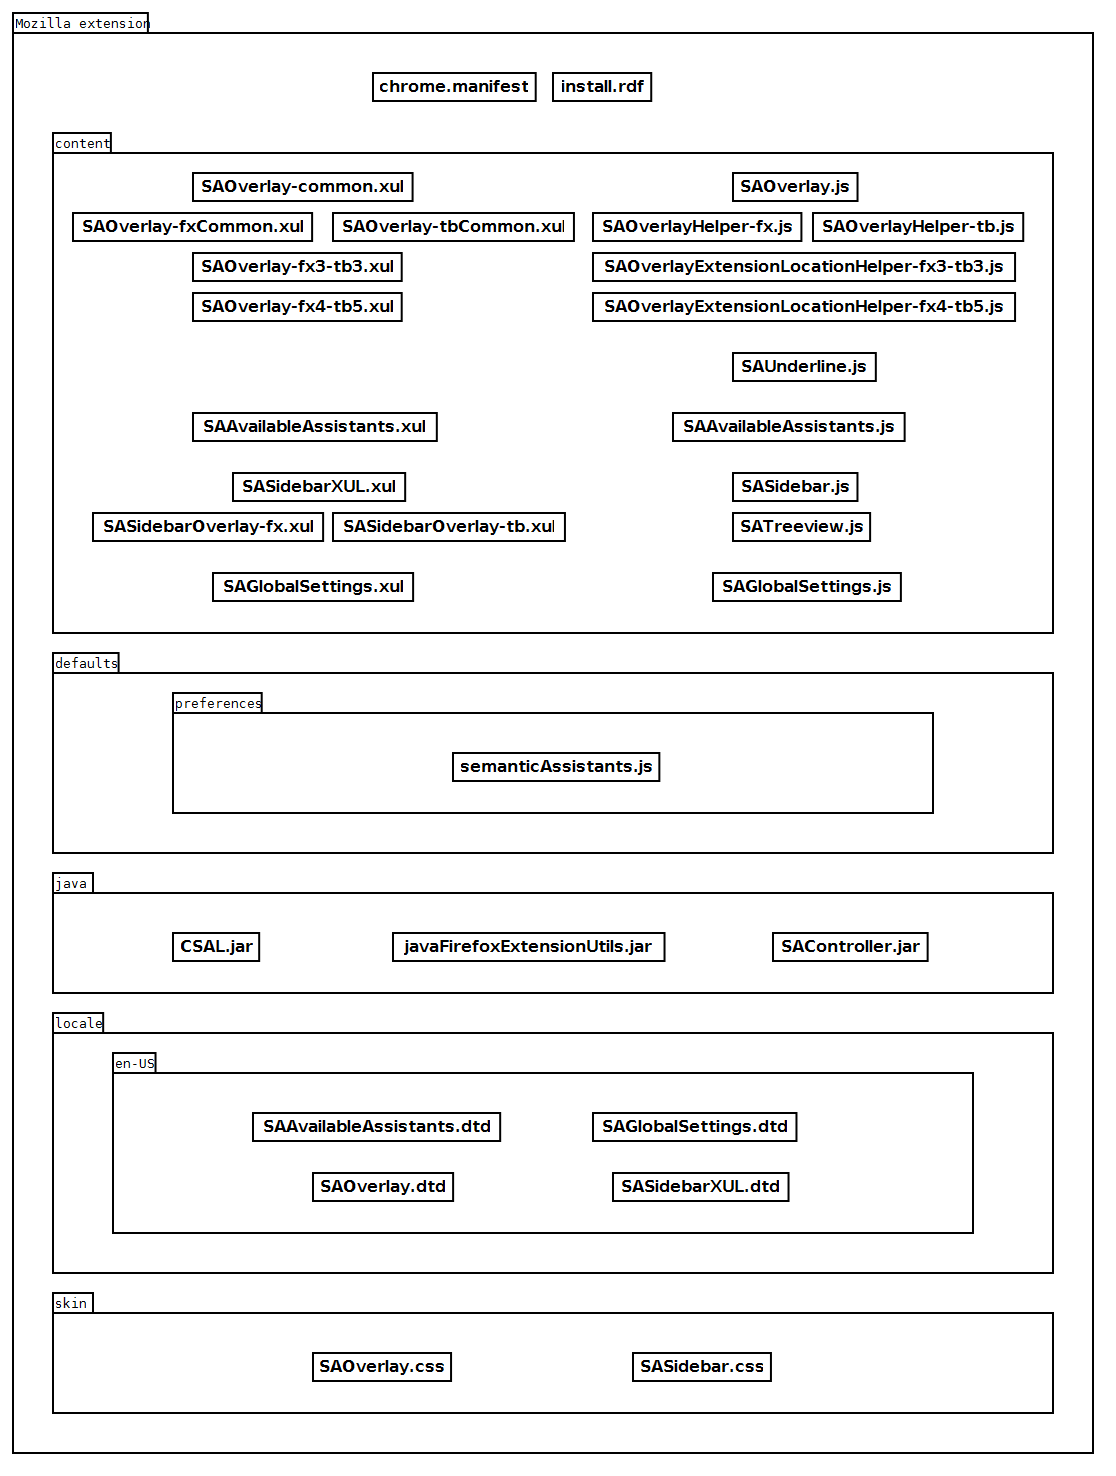
\includegraphics[totalheight=0.8\textheight]{pictures/mozilla_development_notes_file_layout.png}
  \caption{The file layout of the Mozilla extension}
  \label{fig:mozilla_development_notes_file_layout}
\end{figure}

\paragraph{Root folder} At the root of extension folder are two files called ``chrome.manifest" and ``install.rdf". The ``chrome.manifest" identifies the files contained within the extension and also allows to specify which files of the extension are to be loaded, depending on the application and the version of the application on which the extension is running (more on this later). The ``install.rdf" file defines various information about the extension, including the name of the extension (which becomes the name of the aforementioned extension folder), which applications and application versions that the extension is compatible with, and so on. 
\paragraph{The ``content" folder} This contains a series of XUL (.xul) files and JavaScript (.js) files. The XUL files define the user interface elements and behavior, such as windows, dialogs, menus, toolbar buttons. The JavaScript files contain the execution logic, and manipulation of user interface elements. 
\paragraph{The ``defaults" folder} Within the ``defaults" folder is the ``preferences" folder, which contains the default preferences for the extension. Upon installation of the extension, these defaults are set as the preferences in the Firefox/Thunderbird user profile (see above for specifics about preferences). 
\paragraph{The ``java" folder} The ``java" folder contains precompiled Java classes contained within .jar files. The ``CSAL.jar" is the same Client Side Abstraction Layer found in other clients. The ``javaFirefoxExtensionUtils.jar" file is a third-party utility which allows to grant full privileges to Java within a Mozilla extension. The ``SAController.jar" file is the Java component of the extension, which acts as a bridge between the JavaScript code and the CSAL and contains some additional execution logic. 
\paragraph{The ``locale" folder} The purpose of the ``locale" folder is to contain folders that contain files with localized strings used within the extension. These folders are named by specific languages' abbreviations (e.g., ``en-US"). 
\paragraph{The ``skin" folder} The ``skin" folder contains .css files that define layout and appearance properties image resource files for the icons and various UI elements within the extension.

\subsubsection{Compatibility Concerns}
There are differences in the extension between Firefox and Thunderbird. Furthermore, such differences also exist between Firefox 3.6.x and Firefox 4.0 as well as between Thunderbird 3.1.x and Thunderbird 5.0. (There was no Thunderbird 4.0.) This was because major changes were made to the Mozilla platform between those versions of the appliations. 

In order to enable the extension to be compatible with multiple version of Firefox as well as multiple versions of Thunderbird, certain measures were taken. 

Files of the extensions were split such that common code between applications/versions are kept within common files, while code that is different between applications/versions are separated into different versions of the files. The appropriate set of files is loaded for the right application and version. 

The aforementioned ``chrome.manifest" file, located at the root of the extension's folder structure, specifies the files to be loaded for the extension, depending on the application and application version on which the extension is running. Hence, for example, this allows for one file to be loaded for Firefox and another file to be loaded for Thunderbird. Another example would be for one file to be loaded for Firefox version 3.6 and earlier and another file to be loaded for Firefox version 4 and later. 

The files that need to have multiple versions are both the JavaScript files and the XUL files. The JavaScript code may differ between applications/versions due to differences in API. XUL files differ between applications (less for between versions of the same application) due to differences in the user interfaces (different elements, different naming, etc.).

Table~\ref{tab:mozilla_development_files_compatibility} shows which files are used depending on the application and the version of the application. 

\begin{table}[htb]
  \centering\small\sffamily
  \begin{tabular}{p{0.5\textwidth}@{\hspace*{4mm}}p{0.08\textwidth}@{\hspace*{4mm}}p{0.08\textwidth}@{\hspace*{4mm}}p{0.08\textwidth}@{\hspace*{4mm}}p{0.08\textwidth}}
    \toprule
    \textbf{} & \textbf{Fx 3.6.x} & \textbf{Fx 4.0+} & \textbf{Tb 3.1.x} & \textbf{Tb 5.0+} \\
    \midrule
    SAOverlay.js & x & x & x & x \\

    SAOverlayHelper-fx.js & x & x &  &  \\

    SAOverlayHelper-tb.js &  &  & x & x \\

    SAOverlayExtensionLocationHelper-fx3-tb3.js & x &  & x &  \\

    SAOverlayExtensionLocationHelper-fx4-tb5.js &  & x &  & x \\

    SAOverlay-common.xul & x & x & x & x \\

    SAOverlay-fxCommon.xul & x & x &  &  \\

    SAOverlay-tbCommon.xul &  &  & x & x \\

    SAOverlay-fx3-tb3.xul & x &  & x &  \\

    SAOverlay-fx4-tb5.xul &  & x &  & x \\

    SASidebarXUL.xul & x & x & x & x \\

    SASidebarOverlay-fx.xul & x & x &  &  \\

    SASidebarOverlay-tb.xul &  &  & x & x \\
    \bottomrule
  \end{tabular}
  \caption{Files loaded depending on application and version for compatibility}
  \label{tab:mozilla_development_files_compatibility}
\end{table}

\subsubsection{Extension Preferences}
The default preferences of the extension are defined in the folder ``defaults" in the ``preferences" subfolder in the file ``semanticAssistants.js". As previously mentioned, the current settings of those preferences are stored in a file called ``prefs.js" in the user profile folder. 

The preferences are: 

\begin{itemize}
  \item \emph{extensions.semanticAssistants.firstTimeRun} \begin{itemize}
    \item type: boolean
    \item default value: true
    \item This determines whether it is the first time that the extension is launched. If so, it adds the toolbar menu button to the application's main toolbar. 
  \end{itemize}
  \item \emph{extensions.semanticAssistants.installLocation} \begin{itemize}
    \item type: string
    \item default value: ""
    \item This stores the path of the extension. This is not a user preference; it is utilized internally when accessing the .jar files. It is set in the extension when the application's start up. 
  \end{itemize}
  \item \emph{extensions.semanticAssistants.serverCustomHost} \begin{itemize}
    \item type: string
    \item default value: ""
    \item This is a setting set by the user in the ``Global Settings" dialog. 
  \end{itemize}
  \item \emph{extensions.semanticAssistants.serverCustomPort} \begin{itemize}
    \item type: string
    \item default value: "8879"
    \item This is a setting set by the user in the ``Global Settings" dialog. 
  \end{itemize}
  \item \emph{extensions.semanticAssistants.serverDefaultOrCustom} \begin{itemize}
    \item type: integer
    \item default value: 0
    \item 0 for ``Default", 1 for ``Custom"
    \item This is a setting set by the user in the ``Global Settings" dialog. 
  \end{itemize}
\end{itemize}

\subsubsection{Overall Architecture}
The Mozilla extension is composed of three components: the principal component in JavaScript and XUL, the Java component of the extension (contained in the aforementioned ``SAController.jar" file), and the Client Side Abstraction Layer/CSAL (the ``CSAL.jar" file). A high-level representation of the overall architecture is shown in Figure~\ref{fig:mozilla_development_notes_overall_architecture_high_level}).
The main part of the extension is in JavaScript and XUL, as extensions for the Mozilla platform are written in JavaScript code, and the user interface is defined in XUL. A Java component exists in order for the JavaScript component to interoperate with the CSAL; it also adds additional execution logic, such as processing the results from the CSAL. Leveraging a feature in Firefox/Thunderbird called LiveConnect in addition to a third-party package to grant full privileges to Java within a Mozilla extension, the JavaScript code of the extension utilizes and calls the compiled Java code, which in turn utilizes and calls the CSAL. 

\begin{figure}[htb]
  \centering
  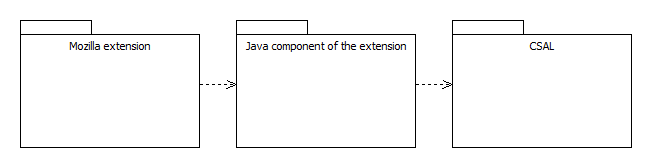
\includegraphics[width=0.8\textwidth]{pictures/mozilla_development_notes_overall_architecture_high_level.png}
  \caption{The overall architecture of the Mozilla extension at a high level}
  \label{fig:mozilla_development_notes_overall_architecture_high_level}
\end{figure}

The main class in the Mozilla extension component is ``SAOverlay" (defined in ``SAOverlay.js" under the ``contents" folder). This class communicates with the other classes in the component. Additionally, it is this class that calls the Java component. The facade for the Java component is the ``SemanticAssistantsController" class. Similarly, the ``SemanticAssistantsController" class is a controller, which coordinates the other classes in the Java component. The various classes of the Java component utilize classes contained within the CSAL. These dependencies are shown in Figure~\ref{fig:mozilla_development_notes_overall_architecture_more_detailed}.

\begin{figure}[htb]
  \centering
  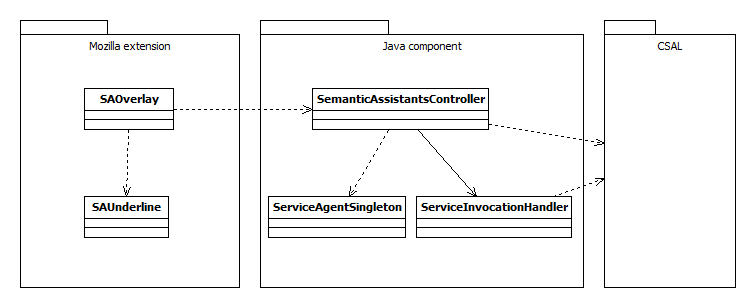
\includegraphics[width=0.8\textwidth]{pictures/mozilla_development_notes_overall_architecture_more_detailed.png}
  \caption{The overall architecture of the Mozilla extension showing some more details in terms of dependencies and showing some of the main modules}
  \label{fig:mozilla_development_notes_overall_architecture_more_detailed}
\end{figure}

\subsubsection{Main Mozilla Extension Component}
The main component of the Mozilla extension consists of a series of JavaScript classes and XUL files. The class diagram in Figure~\ref{fig:mozilla_development_notes_mozilla_extension_class_diagram} shows the main classes and their associations in the main Mozilla extension component as well as the classes called within the Java component. 

\begin{figure}[htb]
  \centering
  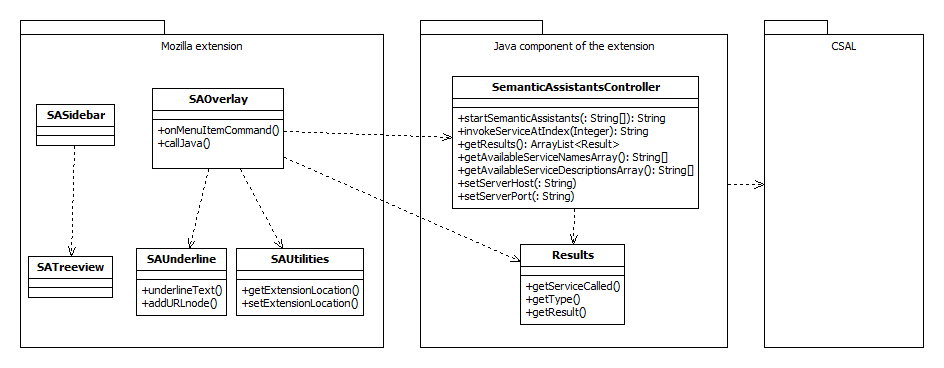
\includegraphics[width=0.95\textwidth]{pictures/mozilla_development_notes_mozilla_extension_class_diagram.png}
  \caption{Class diagram of the main Mozilla extension component}
  \label{fig:mozilla_development_notes_mozilla_extension_class_diagram}
\end{figure}

The main class is ``SAOverlay". When the user invokes the ``Available Assistants" command, it invokes the ``onMenuItemCommand" function in ``SAOverlay". This function obtains the user selection on the page/message, or the whole content of the page/message if no selection was made, and calls the function ``callJava" and passes the user selection. The ``callJava" function then obtains references to the Java classes in the Java component (``SAController.jar"). This is done using the feature called LiveConnect built into Firefox and Thunderbird. Additionally, the aforementioned third-party component ``javaFirefoxExtensionUtils.jar" is required to grant full privileges to the .jar files, as shown in Figure~\ref{list:mozilla_development_notes_main_mozilla_extension_component_jar_permissions}. The method ``startSemanticAssistants" of the ``SemanticAssistantsController" Java class is invoked, and the result returned is a list of available \sa NLP services (``Assistants"). Then, an XUL dialog ``SAAvailableAssistants.xul" is opened, prompting the user to choose an Assistant from the list. 

\begin{figure}
\centering
\begin{lstlisting}[language=Java,numbers=left,xleftmargin=4mm,columns=flexible]
callJava: function(userSelection, allText) {
    var extensionPath = SAOverlay.getExtensionLocation();
    
    var SAControllerJarPath = "file:///" + extensionPath + "/java/SAController.jar"; 
    var classLoaderJarPath = "file:///" + extensionPath + "/java/javaFirefoxExtensionUtils.jar";
    var CSALJarPath = "file:///" + extensionPath + "/java/CSAL.jar";
    
    urlArray = []; 
    urlArray[0] = new java.net.URL(SAControllerJarPath); 
    urlArray[1] = new java.net.URL(classLoaderJarPath);  
    urlArray[2] = new java.net.URL(CSALJarPath);  

    var cl = java.net.URLClassLoader.newInstance(urlArray);

    //set security policies with the policyAdd function defined below
    this.policyAdd(cl, urlArray);
    
    (...)
}, 

(...)

policyAdd: function(loader, urls) {
    try {
        var str = 'edu.mit.simile.javaFirefoxExtensionUtils.URLSetPolicy';
        var policyClass = java.lang.Class.forName(
            str,
            true,
            loader
            );
        var policy = policyClass.newInstance();
        policy.setOuterPolicy(java.security.Policy.getPolicy());
        java.security.Policy.setPolicy(policy);
        policy.addPermission(new java.security.AllPermission());
        for (var j = 0; j < urls.length; j++) {
            policy.addURL(urls[j]);
        }
    }
    catch(e) {
        alert(e+'::'+e.lineNumber);
    }
}
\end{lstlisting}
\caption{Granting full permissions to .jar files inside the extension in the \texttt{callJava} function in the \texttt{SAOverlay} class}
\label{list:mozilla_development_notes_main_mozilla_extension_component_jar_permissions}
\end{figure}

When the selection is made, another method ``invokeServiceAtIndex" of the ``SemanticAssistantsController" Java class is invoked, and upon successful return of the results, the ``getResults" method of the Java class is called to retrieve the results from the service invocation. Then, for each result within the results, an appropriate action is taken. For an ``annotation"-type result, the function ``underlineText" of the ``SAUnderline" JavaScript class is called; for a ``document"-type result, the function ``addURLnode" of ``SAUnderline" is called; for a ``file"-type result, no action is taken, as the Java code executes the opening the file. Save for a ``file"-type result, the ``Semantic Assistants" sidebar, which is the XUL file ``SASidebarXUL.xul", is opened to display the results. 

The sequence diagram in Figure~\ref{fig:mozilla_development_notes_mozilla_extension_sequence_diagram_main_scenario} shows the call sequence involved in the above main scenario of listing the available services and then of invoking a service. 
\begin{figure}[htb]
  \centering
  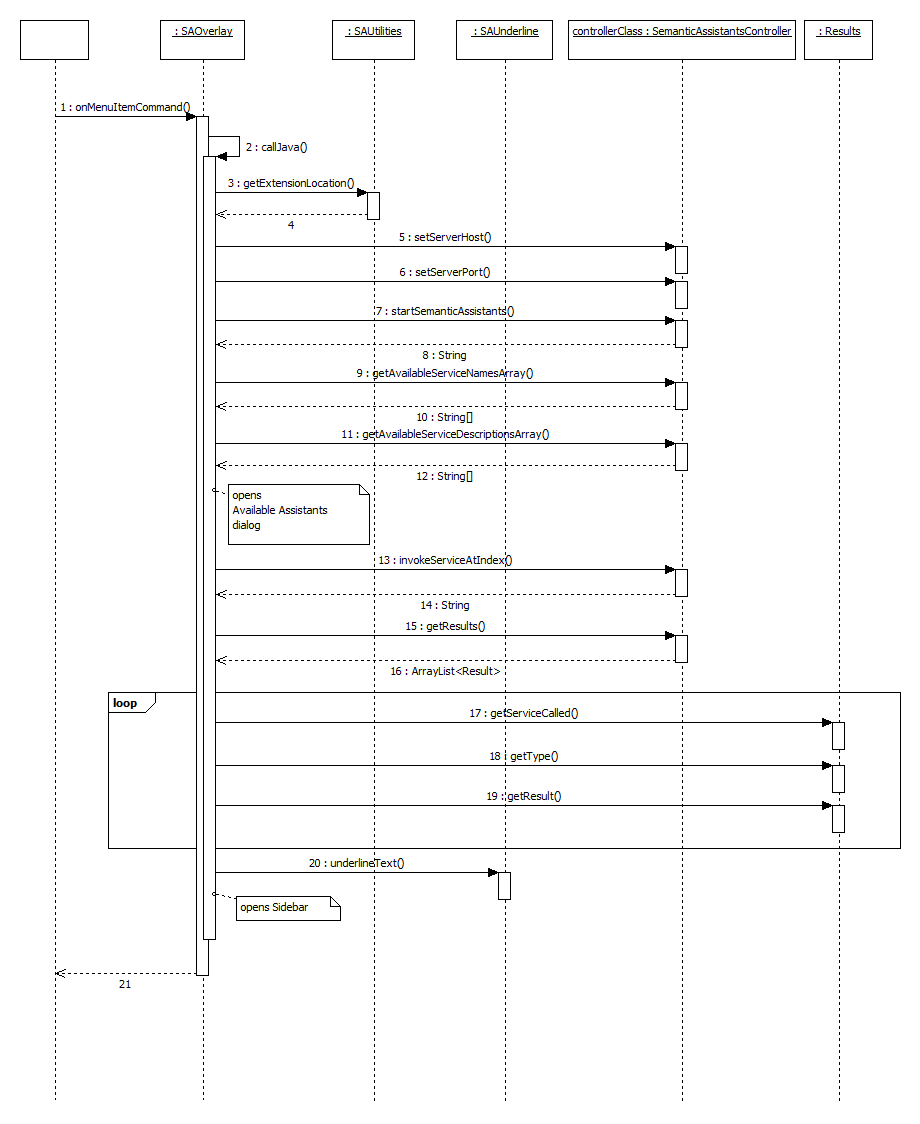
\includegraphics[totalheight=0.8\textheight]{pictures/mozilla_development_notes_mozilla_extension_sequence_diagram_main_scenario.png}
  \caption{Sequence diagram of the main Mozilla extension component for the main scenario}
  \label{fig:mozilla_development_notes_mozilla_extension_sequence_diagram_main_scenario}
\end{figure}

\subsubsection{Java Component}
The Java component consists of a series of Java classes packaged within a .jar file. The class diagram in Figure~\ref{fig:mozilla_development_notes_java_component_class_diagram} shows the principal classes and their associations in the Java component as well as some of the classes in the CSAL called from the Java component. 

\begin{figure}[htb]
  \centering
  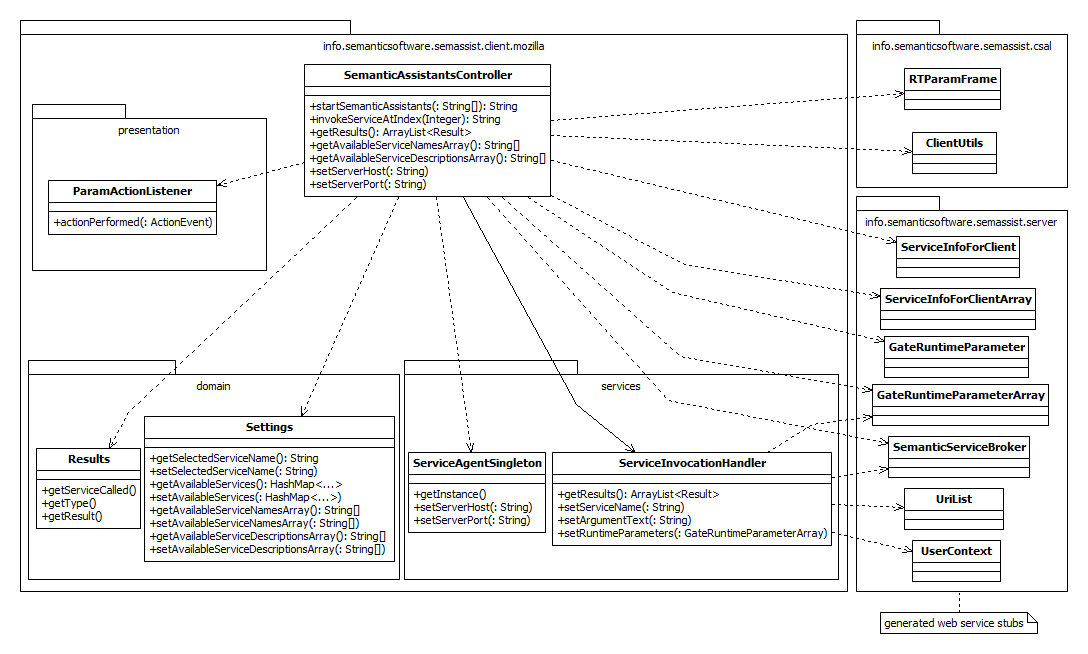
\includegraphics[width=0.95\textwidth]{pictures/mozilla_development_notes_java_component_class_diagram.png}
  \caption{Class diagram of the Java component}
  \label{fig:mozilla_development_notes_java_component_class_diagram}
\end{figure}

The main class is ``SemanticAssistantsController"; it is the facade class of the Java component packaged within ``SAController.jar" file and acts as a controller that calls and coordinates all other classes. 

\paragraph{The scenario of getting available services} The method ``startSemanticAssistants" of the ``SemanticAssistantsController" class is called. By calling ``getInstance" of ``ServiceAgentSingleton", a ``SemanticServiceBroker" instance is obtained. Calling ``getAvailableServices" of the latter returns a ``ServiceInfoForClientArray", which is a collection of the available services from the server. Then, these available services are stored in the ``Settings" class, as well as service names and service descriptions to be utilized by the main JavaScript component to display to the user. (A code snippet of this can be seen in Figure~\ref{list:mozilla_development_notes_java_component_get_available_services}.)

The sequence diagram in Figure~\ref{fig:mozilla_development_notes_java_component_sequence_diagram_get_available_services} shows the call sequence in the above scenario of obtaining the list of available services from the server. 

\begin{figure}
\centering
\begin{lstlisting}[language=Java,numbers=left,xleftmargin=4mm,columns=flexible]
SemanticServiceBroker agent = ServiceAgentSingleton.getInstance();
ServiceInfoForClientArray sia = agent.getAvailableServices();

List<ServiceInfoForClient> results = sia.getItem();
Iterator<ServiceInfoForClient> it = results.iterator();

(...)

while( it.hasNext() ) {
    ServiceInfoForClient info = it.next();
    availableServices.put( info.getServiceName(), info );
    (...)
}

(...)

Settings.setAvailableServices( availableServices );
\end{lstlisting}
\caption{Getting the available services in the the \texttt{startSemanticAssistants} method in the \texttt{SemanticAssistantsController} class}
\label{list:mozilla_development_notes_java_component_get_available_services}
\end{figure}

\begin{figure}[htb]
  \centering
  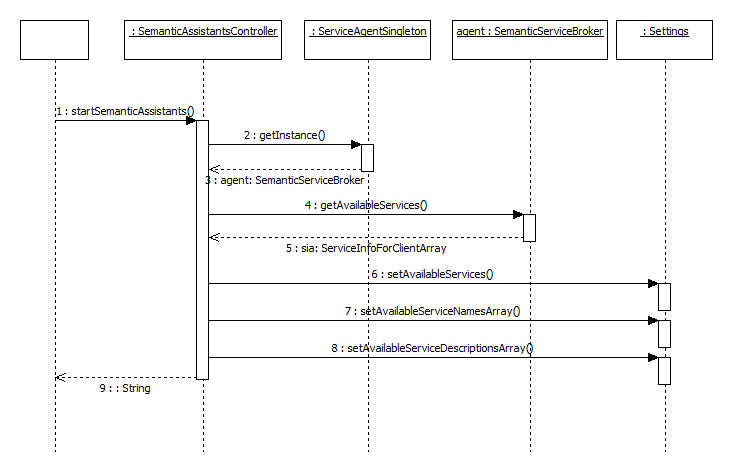
\includegraphics[width=0.95\textwidth]{pictures/mozilla_development_notes_java_component_sequence_diagram_get_available_services.png}
  \caption{Sequence diagram of the Java component for the scenario of getting available services}
  \label{fig:mozilla_development_notes_java_component_sequence_diagram_get_available_services}
\end{figure}

\paragraph{The scenario of invoking an available service} The method ``invokeServiceAtIndex" of the ``SemanticAssistantsController" class is called with the argument passed from the JavaScript code specifying which service was specified by the user. The name of the service, which is what is used to identify services, is determined. The method ``runSelectedService" is called, where the ``ServiceInfoForClient" corresponding to the service is retrieved from the list saving during the ``startSemanticAssistants" method call. 

If this service has parameters to be entered by the user, these parameters are retrieved based on the service and displayed in a ``JFrame" for the user to enter the required and optional parameters. 

A new ``GateRuntimeParameterArray" instance, containing the user input for the parameters if there were any, is passed to ``doRunSelectedService" method. In this method, the service name and text to be analyzed are set in a newly instantiated ``ServiceInvocationHandler" is instantiated, then ``getResults" is called. In this method, from ``ServiceAgentSingleton", ``SemanticServiceBroker" instance is obtained; ``invokeService" of this instance is called upon while passing the service name, the text to be analyzed, the parameters (if any), as well as other arguments. The result returned is a string which when processed by the ``getServiceResults" method of ``ClientUtils" yields a list of ``SemanticServiceResult" results. Then, each result is processed according to its result type. For example, for a "file"-type result, code is run to open the file in the Web browser; for a "annotation"- or "document"-type result, the result is set appropriately in the list of results returned to the JavaScript code, to be then processed by the main extension component. 

The sequence diagram in Figure~\ref{fig:mozilla_development_notes_java_component_sequence_diagram_invoke_service} shows the call sequence in the above scenario of invoking an available service from the server and obtaining the results. 

\begin{figure}[htb]
  \centering
  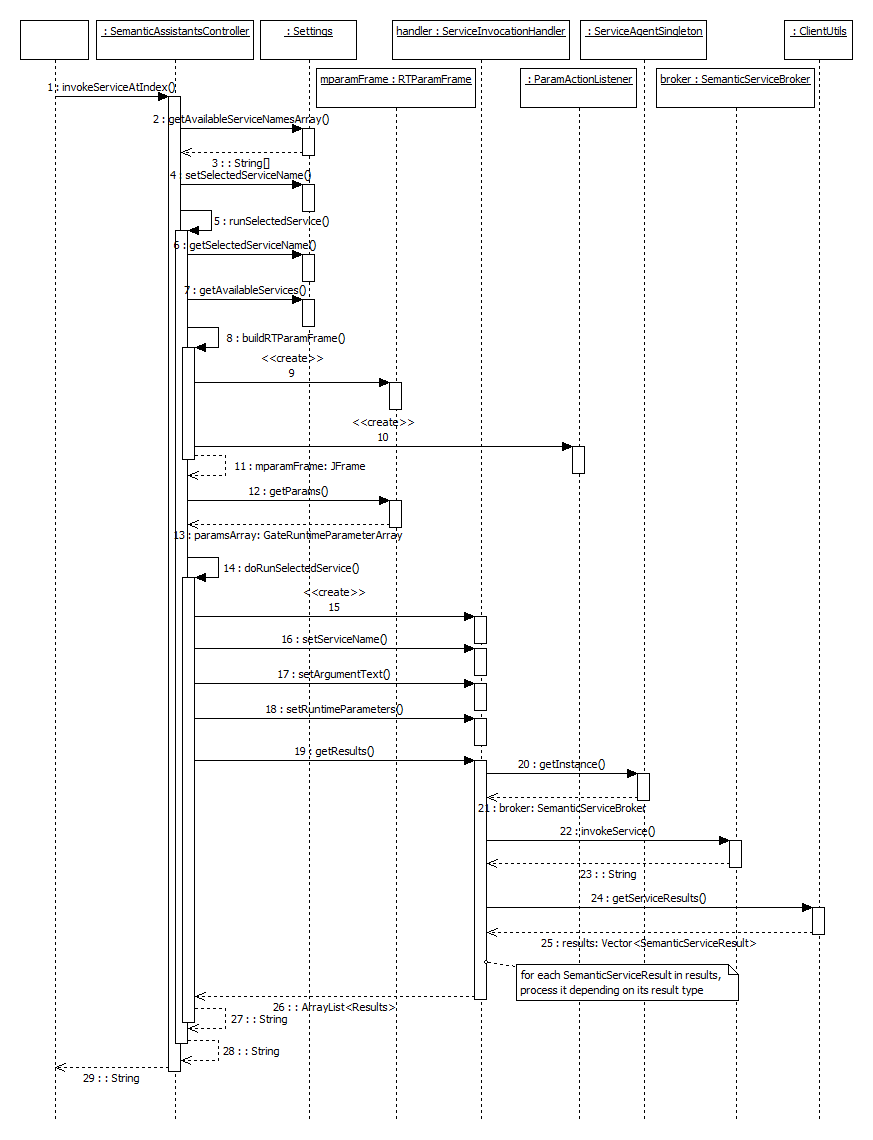
\includegraphics[totalheight=0.8\textheight]{pictures/mozilla_development_notes_java_component_sequence_diagram_invoke_service.png}
  \caption{Sequence diagram of the Java component for the scenario of invoking a service}
  \label{fig:mozilla_development_notes_java_component_sequence_diagram_invoke_service}
\end{figure}

\section{Android Application}
Mobile phones use a variety of operating systems that transform them from a traditional handheld device for talking into general-purpose computing platforms. Android OS\footnote{Google's Android Platform~\url{http://developer.android.com}}, is an open source platform for mobile and tablet development led by Google Inc. It is a comprehensive Linux-based platform that supports most of the Java Platform and features its own extensive user interface framework. This platform is widely used by programmers to create applications and games for handheld devices. We have leveraged this platform to create an application that allows users to use novel NLP solutions inside their devices. This app, henceforth referred to as the \sa App, not only can be used as a standalone application, but also plays the role of a system-wide NLP service provider for other applications. Note that the \sa App was originally implemented based on Android 3.0 Platform\footnote{Android 3.0 Platform,~\url{http://developer.android.com/sdk/android-3.0.html}} (Honeycomb) but its backward compatibility has also been tested with Android 2.2. It is, however, recommended that the app be used in Android 3.0+ versions.

In the following sections, we describe the \sa App features and provide a guide on how to use the \sa App services inside external applications.

\subsection{Features}
The user interface shown in Figure~\ref{fig:android_main} is the \sa main activity (user interface). This means that once the app is installed on the device, this is the main entry to the application. It allows users to connect to a specific \sa server and invoke an assistant on the provided text input.

\begin{figure}[htb]
\centering
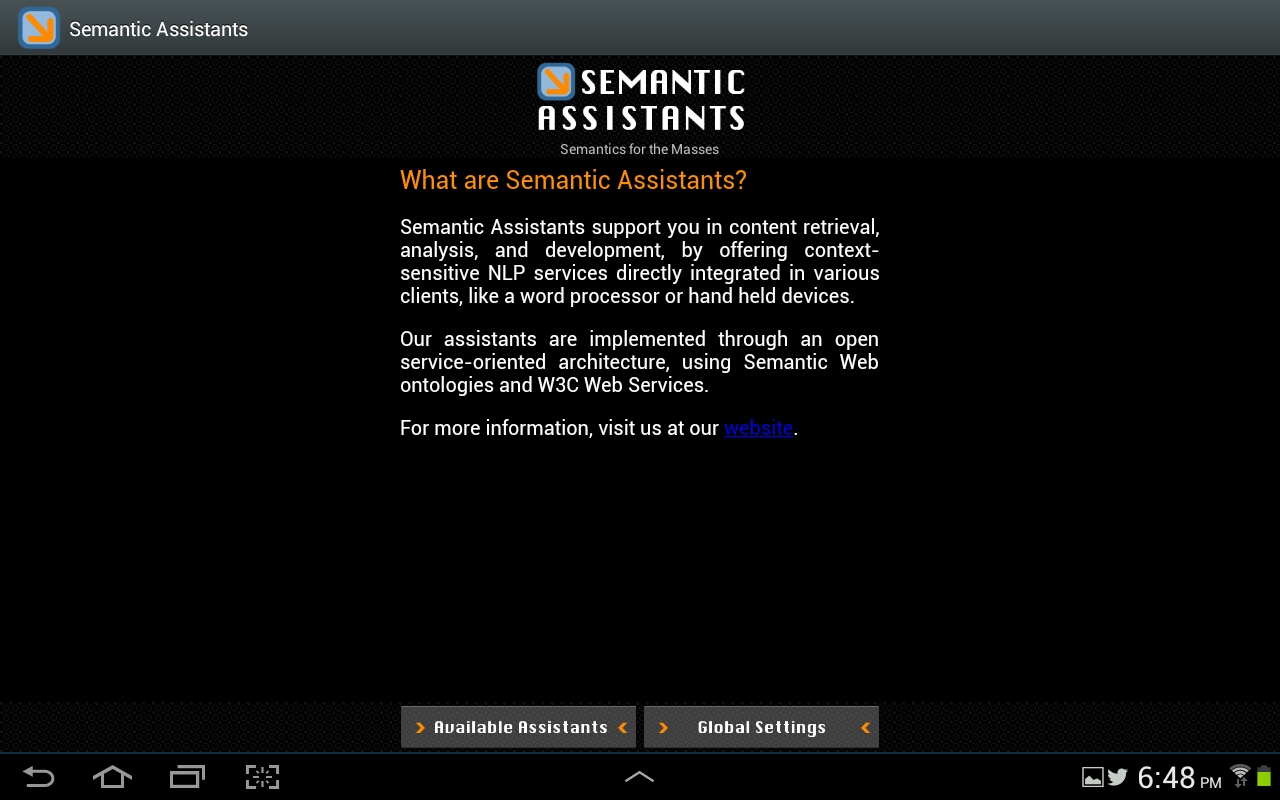
\includegraphics[scale=0.35]{pictures/android_main.jpg}
\caption{\sa Android App Main Activity}
\label{fig:android_main}
\end{figure}
\subsubsection{\sa Account}
Each android-enabled device has at least one built-in account type, i.e., the Google account. Android is designed in such a way that the same account can be registered to a variety of account-based services. For example, the Gmail account that is set up on the Android device is not just used for e-mailing , but for all the Google account-based applications. The same concept applies to the \sa App that uses the \emph{\sa account} type for its applications. Just like another accounts, you first need to sign up for a \sa Account before using the application.

Once you have obtained your credentials, on your device browse to \texttt{Settings $\rightarrow$ Accounts and Sync $\rightarrow$ Add Account} and choose the ``\sa'' option from the list. In the provided user interface, type in your \sa accounts credentials and press \texttt{Sign in}. If authenticated successfully, your \sa account will appear in the list of your device accounts.

\blankline
\noindent
\textbf{Note:} Before authenticating or signing up for an account, you need to choose the \sa server where your account is located. For this, follow the instructions in Section~\ref{sec:android_global_settings}.

\subsubsection{Global Settings}
\label{sec:android_global_settings}
Similar to other \sa clients, the \sa App allows users to connect to various arbitrary servers to inquire about their available assistants. On the \sa App main activity, press the \texttt{Global Settings} button. The application settings activity will pop up that allows you to define a new server location or choose one from a list of available servers as shown in Figure~\ref{fig:android_global_settings}.

\begin{figure}[htb]
\centering
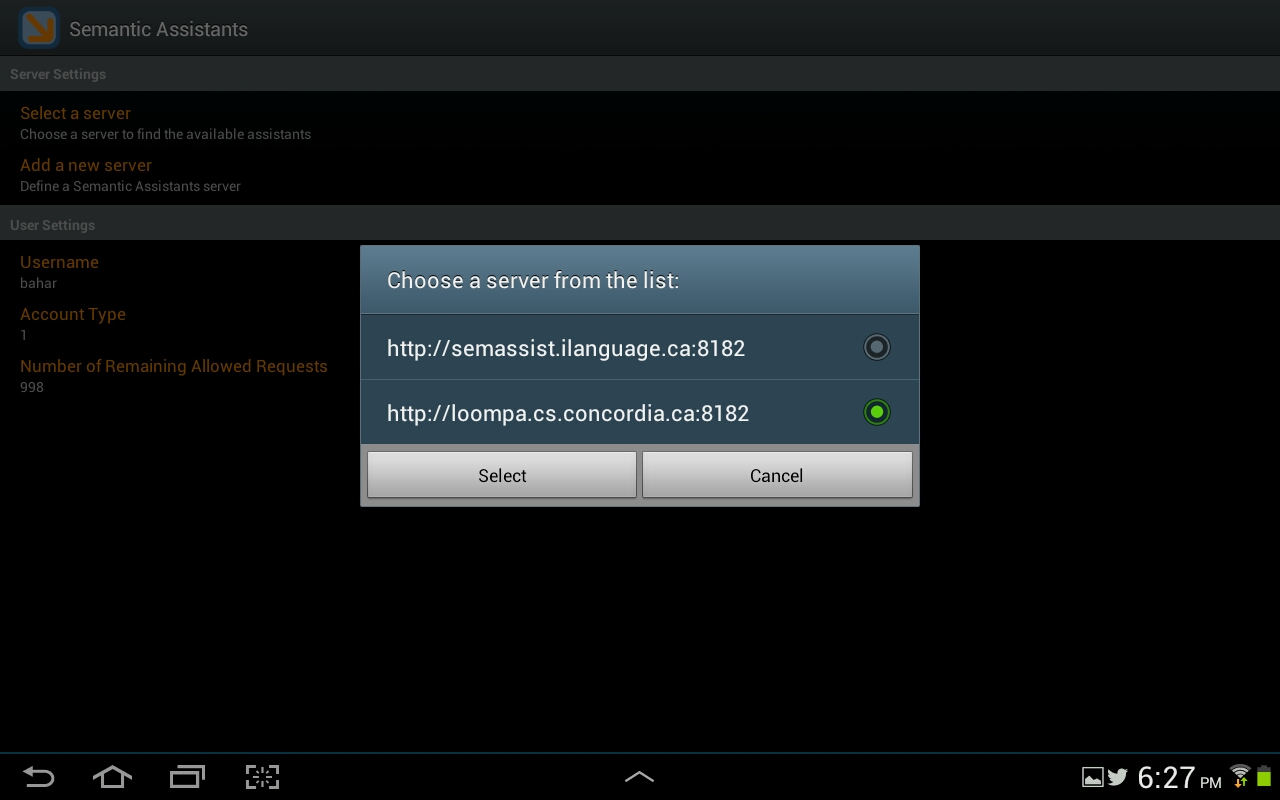
\includegraphics[scale=0.35]{pictures/android_global_settings.jpg}
\caption{\sa App Global Settings Activity}
\label{fig:android_global_settings}
\end{figure}

In order to add a new server location, click on the \texttt{Add a new server} option and type in the server URL by concatenating the server address, including its protocol and port number, like in Figure~\ref{fig:android_new_server}. In order to choose the newly defined server, choose the \texttt{Select a server} option from the Global Settings activity and select it from the list.

\begin{figure}[htb]
\centering
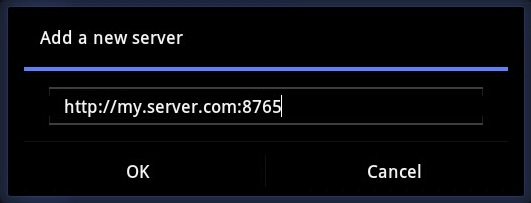
\includegraphics[scale=0.5]{pictures/android_new_server.jpg}
\caption{Adding a new server to the \sa App settings}
\label{fig:android_new_server}
\end{figure}

\subsubsection{NLP Service Invocation}
Once the \sa server is selected from the Global Settings activity, users can inquire about its available assistants. From the \sa App main activity, press the \texttt{Available Assistants} button to open the service invocation activity. This activity, as shown in Figure~\ref{fig:android_invoke_main}, presents the list of available assistants and an input text area for the text to be analyzed. By selecting each assistants from the list, the app will provide detailed information of what the assistant does and allows to customize the pipeline execution through providing runtime parameters.

\begin{figure}[htb]
\centering
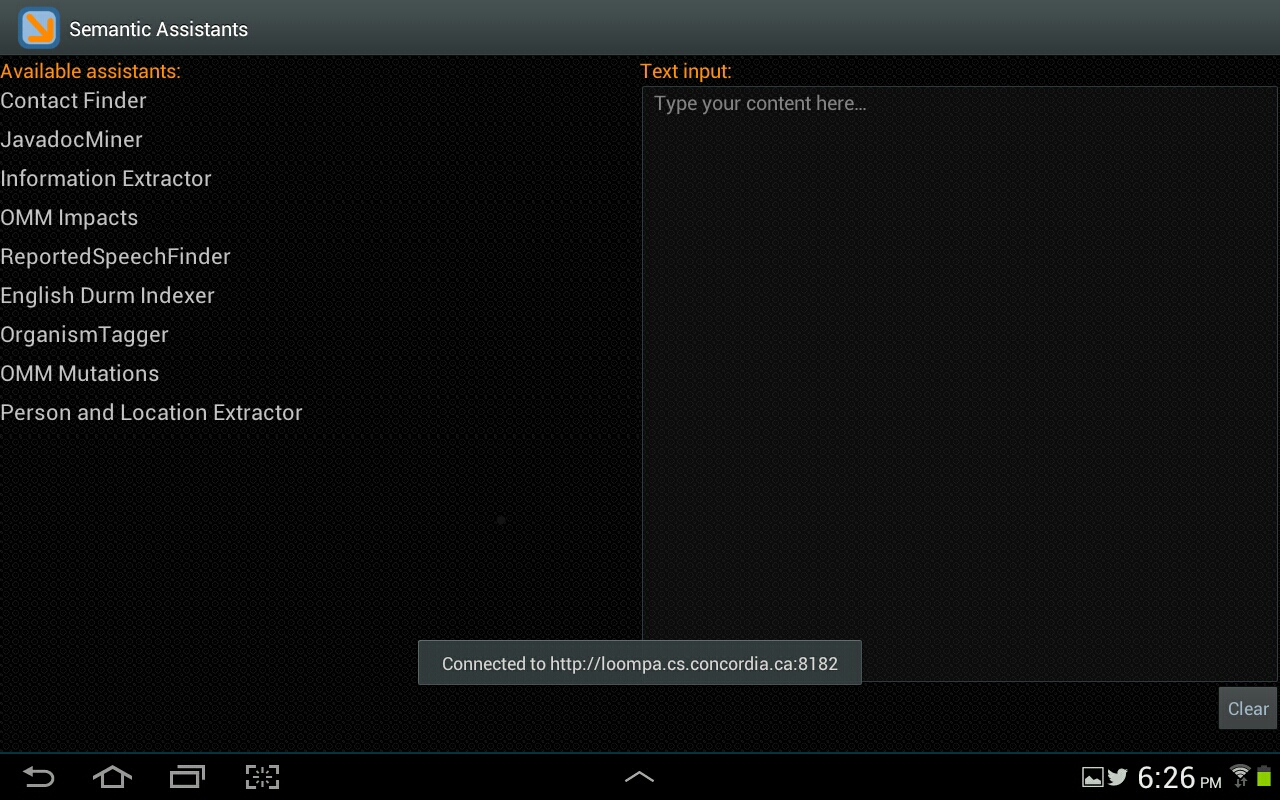
\includegraphics[scale=0.35]{pictures/android_invoke_main.jpg}
\caption{Adding a new server to the \sa App settings}
\label{fig:android_new_server}
\end{figure}

Users have three options on how to provide a pipeline with text input:
\begin{itemize}
\item{\textbf{Manually typing in the text. }}{Using the device keyboard, type in the text that is to be analyzed.}
\item{\textbf{Sharing text with the \sa from other apps. }}{The \sa App listens for sharing event in the Android platform. This means that from within applications that provide a sharing mechanism, the selected text can be directly placed into the \sa Apps activity input.}
\item{\textbf{Sending input to the \sa service. }}{As we will explain more in Section \ref{sec:android_service}, the text input can be sent via a service argument (extra). The difference between this option and the previous bullet is that in the sharing option, the \sa App takes care of the result handling instead of the invoking application. Also in this service invocations, the NLP service to be executed is pre-defined and cannot be changed at a later stage.}
\end{itemize}
Once done with typing, select an assistants from the left-side list and press the \texttt{Invoke} button. Depending on the type of the results, you would either see the annotations in a new activity or the resulting file will be opened in the device browser.

\subsection{Installation}
TBD

\subsection{\sa App Service}
\label{sec:android_service}
As mentioned earlier, the \sa App also plays the role of a system-wide service provider, meaning that other external applications can use the \sa App's functionality. This is done through using Android services, i.e., application components that can perform long-running operations in the background. Each available service in the \sa App has a unique name that should be indicated when the external application invokes the service.

To better demonstrate this feature, we will illustrate a demo app that uses a \sa service. The demo in example, called iForgotWho, is an app that helps users to find potential ``contacts'' from a given text and upon user accept, automatically adds them to the device contact book. However, the iForgotWho app does not find the contacts by itself, rather it uses the \sa App's \texttt{person\_extractor} service. For this, the iForgotWho needs to (1) invoke the service using its complete identifier (available in the \sa App manifest file), (2) send along the text to be analyzed, and (3) indicate whether the \sa App should present the results or iForgotWho takes care of it. Once all the data is provided to the \sa App, the NLP service is executed and the results are passed back to iForgotWho app. Then, iForgotWho presented the list of all the person entities found in the text to the user, whom which ultimately decide whether they should be added to the device contact book. Figure~\ref{fig:android_service} illustrates this sequence.

\subsection{Development Notes}
In this section, we provide technical notes about the \sa App and how external Android application developers can integrate NLP capabilities in their apps using the \sa services.

\subsubsection{Extending the \sa App}
The \sa App source directory is structured as follows:
\begin{enumerate}
\item\url{activity}: This folder contains the classes representing graphical user interfaces.
\item\url{application}: This folder contains the \sa App's main application class and provides a static access to its context.
\item\url{business}: This folder contains the classes that handle communication with the \sa server.
\item\url{encryption}: This folder contains classes that take care of the secure HTTP connection attributes, such as the SSL certificate.
\item\url{intents}: This folder contains the intents factory class used by \sa App's services.
\item\url{parser}: This folder contains the parsers for Restful request and response representations.
\item\url{prefs}: This folder contains the utility classes for Android preference management.
\item\url{service}: This folder contains the authentication and service invocation service listeners.
\item\url{utils}: This folder contains the app's utility classes.
\end{enumerate}

In order to extend the \sa App, import the \sa App to your Eclipse or other IDE of choice. Note that you need to have the Android SDK\footnote{Android SDK, \url{http://developer.android.com/sdk/}} specific to your operating system installed on your machine.

\subsubsection{Using the \sa App Service}
In order integrate the \sa App service in your application, you have to first find the exact service name in the \sa App's manifest. For example, in order to detect Person named entities in a text, you have to call the \texttt{org.openintents.action.PERSON\_EXTRACTOR} service, using this code:

\begin{lstlisting}[language=Java,numbers=left,xleftmargin=4mm,columns=flexible]
 // specify which service should be invoked
 Intent service = new Intent(org.openintents.action.PERSON_EXTRACTOR);

 // the text to be analyzed
 String input = "I met John Smith at a conference last year.";

 // set the service input
 service.putExtra(Intent.EXTRA_TEXT, input);

 // let the Semantic Assistants App know the invoking app will present the results
 service.putExtra("SILENT_MODE", "true");

 // call the service
 startService(service);
\end{lstlisting}

You also have to define a Broadcast Receiver\footnote{Android Broadcast Receiver, \url{http://developer.android.com/reference/android/content/BroadcastReceiver.html}} to get back the results from the \sa App once the service results are ready. In your broadcast receiver class, you can then decide on how to present the results. Note that what the \sa App returns is the XML representation of the NLP pipeline as discussed in Section~\ref{sec:response}.

\subsubsection{Adding More ServiceIntents}
You can also easily add more services to the \sa App. In order to add a new service you must take the following steps:

\blankline
\noindent
\textbf{Step 1: Add the service name to list of available services. } In order to inform the \sa App of the newly added service, you need to add the unique name of the service as an \texttt{intent-filter} to the \texttt{service} node in the \sa App's manifest file. Specifically, you should add these lines to the \texttt{AndroidManifest.xml} file:

\begin{lstlisting}[language=XML,numbers=left,xleftmargin=4mm,columns=flexible]
<service android:name="info.semanticsoftware.semassist.android.service.SemanticAssistantsService"
		 android:process=":semassist_service" 
		 android:label="semassist">
	<intent-filter android:label="A_LABEL_FOR_YOUR_SERVICE">
		<action android:name="com.example.action.YOUR_SERVICE_NAME" />
		<category android:name="android.intent.category.DEFAULT" />
	</intent-filter>
</service>
\end{lstlisting}

Adding this line to the manifest allows the \sa App to receive the service requests from external applications.

\blankline
\noindent
\textbf{Step 2: Create the class that handles the results. }
Next is to create the class that will perform the actual service execution and handles the server response. This new class must extend the \texttt{ServiceIntent} class in the \texttt{intents} package and must have a \texttt{execute{}} method. In your execute method, you should let the parent class handle the actual service execution and instead handle the response before sending it back to the invoking app. The following snippet shows the service class for the \texttt{PERSON\_EXTRACTOR} service:

\begin{lstlisting}[language=Java,numbers=left,xleftmargin=4mm,columns=flexible]
public class PersonExtractorIntent extends ServiceIntent{

	// the exact service name as specified in its OWL file
	private final static String PR_NAME = "Person and Location Extractor";

	public PersonExtractorIntent(){
		super(PR_NAME);
	}

	public String execute() {
		//STEP1: Execute the service
		String rawResults = super.execute();

		//STEP2: Filter the results
		try{
			String filteredResult = "";
			// remove anything but "Person" annotations from the rawResults
			...
		} catch (Exception e){
			// handle exception
			....
		}
		return filteredResults
	}
}
\end{lstlisting}

\blankline
\noindent
\textbf{Step 3: Update the factory class. }
Finally let the \texttt{ServiceIntentFactory} class know how to map a service request to its corresponding handling class by adding the service action name to its enumeration class:

\begin{lstlisting}[language=Java,numbers=left,xleftmargin=4mm,columns=flexible]
/** Enumeration class for service intents */
enum Intents {person_extractor, YOUR_SERVICE_NAME};
\end{lstlisting}

\blankline
\noindent
and update the switch statement:

\begin{lstlisting}[language=Java,numbers=left,xleftmargin=4mm,columns=flexible]
switch(Intents.valueOf(action.toLowerCase())){
	case person_extractor:
		return new PersonExtractorIntent();
	case your_service_name
		return new YourServiceIntent();
	default:
		return null;
	}
\end{lstlisting}

\section{Global Preference Management}
\label{sec:pref_management}
Semantic Assistants clients preferences are stored in a single hidden file in the user machine's home directory under the name \texttt{semassist-settings.xml}. This file is shared between all the clients and contains information, such as different servers that clients can connect to as well as other client-specific preferences. The preference XML document has two main parts: a global part and a client-specific part. The scope of the global preference, as the name suggests, is all of the clients and any changes to this part will affect them all. The client-specific scope, on the other hand, is limited to that specific client and does not affect others. Each Semantic Assistants client installed on the user machine has a dedicated tag inside the client-specific part, where it can store its proprietary preferences.

This file does not ship with the Semantic Assistants project but a default preference file is created by the very first client installed and used on the user's machine and will be reused by the subsequent clients. It is not advised to manually modify this file unless its structure can be kept consistent. In case of deletion, a default file will be again created by the next used client. The structure of the preference file is detailed in \ref{client_pref}.
% Semantic Assistants - http://www.semanticsoftware.info/semantic-assistants
%
% This file is part of the Semantic Assistants architecture.
%
% Copyright (C) 2009, 2010, 2011, 2012, 2013 Semantic Software Lab, http://www.semanticsoftware.info
% The Semantic Assistants architecture is free software: you can
% redistribute and/or modify it under the terms of the GNU Affero General
% Public License as published by the Free Software Foundation, either
% version 3 of the License, or (at your option) any later version.
%   
% This program is distributed in the hope that it will be useful,
% but WITHOUT ANY WARRANTY; without even the implied warranty of
% MERCHANTABILITY or FITNESS FOR A PARTICULAR PURPOSE.  See the
% GNU Affero General Public License for more details.
% 
% You should have received a copy of the GNU Affero General Public License
% along with this program.  If not, see <http://www.gnu.org/licenses/>.


\chapter{Command-Line Client}
\label{sec:sacl:clc}
This is a simple example client to access the server from the command line.
It is located under \url{SemanticAssistants/Clients/CommandLine} and is meant to demonstrate and test to plug-in developers various Semantic Assistant functionalities.

\begin{enumerate}
\item To compile: \emph{ant compile}
\item To run: \emph{./runclient.sh}
\end{enumerate}

The \texttt{runclient.sh} script helps with the
class path setting, but also adds some difficulty with getting quotes right
when passing parameters to the program. For example, to list all
available services, you can run
\begin{verbatim}
    ./runclient.sh listall
\end{verbatim}
to query the server for all available NLP services. For the default
installation, you should see an output like:
\begin{verbatim}
    Retrieving service info from server...   done
    Listing services:
    Yahoo Search
    IR Information Extractor
    Person and Location Extractor
\end{verbatim}
Now you can invoke one of the services. For example, to extract all
person and location entities from a Wikipedia article, you can run
\begin{verbatim}
    ./runclient.sh invoke "\"Person and Location Extractor\"" \
    "docs=http://en.wikipedia.org/w/index.php?title=Christiane_Kubrick&printable=yes"
\end{verbatim}
If everything works, you will see the raw service response (in XML
format).  Note again that the server has to be running and both the
CSAL and command-line client must have been compiled successfully.

\section*{Connecting to any Server}
The user is able to specify the Server information (Host and Port) of
a local or distant server.  To achieve that the \url{params} part of the
command needs to be used.  The only extra info needed is appending the
following string to the end of the command:
\begin{verbatim}
    "params=(Host=<target Host>,Port=<target server port>)"
\end{verbatim}

For example:
\begin{verbatim}
    "params=(Host=localhost,Port=8080)"
\end{verbatim}

This parameter list may be added at every invocation.

\section*{Configuring Client Preferences}
The Semantic Assistant CSAL architecture makes it is possible to configure persistent server connection and runtime preferences for the command-line client via the \texttt{semassist-settings.xml} file described in section \ref{sec:pref_management}.
Run the following to see all configurations relevant to the command-line client. The output should be similar to this:
\begin{verbatim}
    ./runclient.sh listpref

    global preferences:
    lastCalledServer.port=8879
    lastCalledServer.host=minion.cs.concordia.ca
    server.port=8879
    server.host=minion.cs.concordia.ca
    server.port=8879
    server.host=assistant.cs.concordia.ca

    cmdline preferences:
\end{verbatim}

To then create new or override existing preferences in either the global or the client scopes, you can run something like the following:
\begin{verbatim}
    ./runclient.sh setpref cmdline server.host=localhost
    ./runclient.sh setpref cmdline server.port=8080
\end{verbatim}
Note that while any preference can be configured, only supported ones will take effect for the command-line client.
Only the following preferences are currently supported: \texttt{server.host}, \texttt{server.port}, \texttt{lastCalledServer.host} and \texttt{lastCalledServer.port}.



% Semantic Assistants - http://www.semanticsoftware.info/semantic-assistants
%
% This file is part of the Semantic Assistants architecture.
%
% Copyright (C) 2009, 2010, 2011, 2012 Semantic Software Lab, http://www.semanticsoftware.info
% The Semantic Assistants architecture is free software: you can
% redistribute and/or modify it under the terms of the GNU Affero General
% Public License as published by the Free Software Foundation, either
% version 3 of the License, or (at your option) any later version.
%  
% This program is distributed in the hope that it will be useful,
% but WITHOUT ANY WARRANTY; without even the implied warranty of
% MERCHANTABILITY or FITNESS FOR A PARTICULAR PURPOSE.  See the
% GNU Affero General Public License for more details.
% 
% You should have received a copy of the GNU Affero General Public License
% along with this program.  If not, see <http://www.gnu.org/licenses/>.


\chapter{OpenOffice/LibreOffice Writer Plug-In}
%TODO: update screenshots
The OpenOffice/LibreOffice application suite offers a mechanism
to add application extensions, or plug-ins. We used this
mechanism to integrate OpenOffice.org's word processing
application Writer with our architecture, and thus equip the
Writer with Semantic Assistants \citep{giwi08}.

Our primary goal for the Writer extension was to be able
to perform text analysis on the current document. This
text can, for instance, be a large document from which
information should be extracted, or a problem statement
consisting of a few questions, which serves as input for a
question-answering (QA) Semantic Assistant. Especially
for the last use case, it must allow a user to highlight part of
a document (e.g., a question) and be able to pass only the
highlighted part as input to a language service. Furthermore,
the extension must offer the possibility to specify parameters
that need to be passed to a selected NLP service.

An OpenOffice.org plug-in is basically a zip file with specific
contents and certain descriptions of these contents.  For a detailed
description of the implementation please refer to
Section~\ref{sec:oo-spec}. \textbf{Note:} The current version of the
plug-in requires at least OpenOffice.org Version 3.1.


\section{Features}
Our plug-in creates a new menu entry ``Semantic Assistants:''
\begin{center}
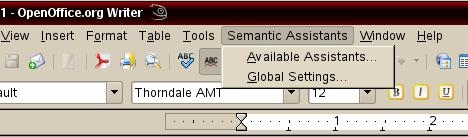
\includegraphics[width=0.7\textwidth]{pictures/oomenu.jpg}
\end{center}

In this menu, the user can inquire about available services, which are
selected based on the client (here \emph{Writer}) and the language
capabilities of the deployed NLP services (described in service
metadata, see Section~\ref{sec:owl}). The dynamically generated list
of available services is then presented to the user, together with a
brief description, in a separate window, as shown in
Figure~\ref{fig:oolist}. Note that the integration of a new service
does not require any changes on the client side---any new NLP service
created and deployed by a language engineer is dynamically discovered
through its OWL metadata maintained by the architecture and so becomes
immediately available to any connected client.
\begin{figure}[htb]
  \centering
  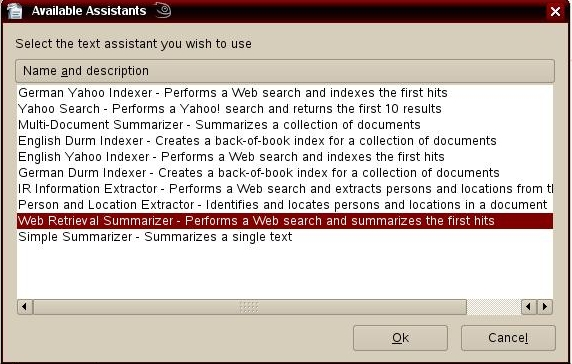
\includegraphics[width=0.5\textwidth]{pictures/oolist.jpg}
  \caption{List of available semantic assistants}
  \label{fig:oolist}
\end{figure}

The user can now select an assistant and execute it. In case the
service requires additional parameters, such as the length of a
summary to be generated, they are detected by our architecture through
the OWL-based service description and requested from the user through
an additional dialog window. An example, for the \emph{Web Retrieval
  Summarizer} assistant, is shown in Figure~\ref{fig:ooparams}.
\begin{figure}[htb]
  \centering
  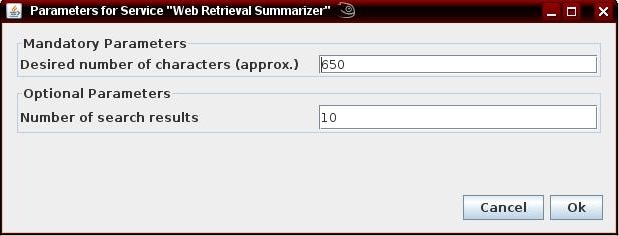
\includegraphics[width=0.5\textwidth]{pictures/ooparams.jpg}
  \caption{The parameters dialog, which appears when a Semantic
    Assistant requiring further input is invoked}
  \label{fig:ooparams}
\end{figure}
After the service is executed, the result is displayed in Writer depending on
the type of the server response: either as a new document, as annotations on
the existing document, or by opening an external viewer (e.g., a Web browser
for HTML documents).

\subsection{Side-Notes View}
The latest release of the OpenOffice.org Suite offer a new feature for text
annotation.  Depending on the annotation results received from GATE, the
Semantic Assistants Writer plug-in presents it in a sidenote manner (see
Figure~\ref{fig:sidenotes}).
\begin{figure}[htb]
  \centering
  %\vspace*{-9mm}
  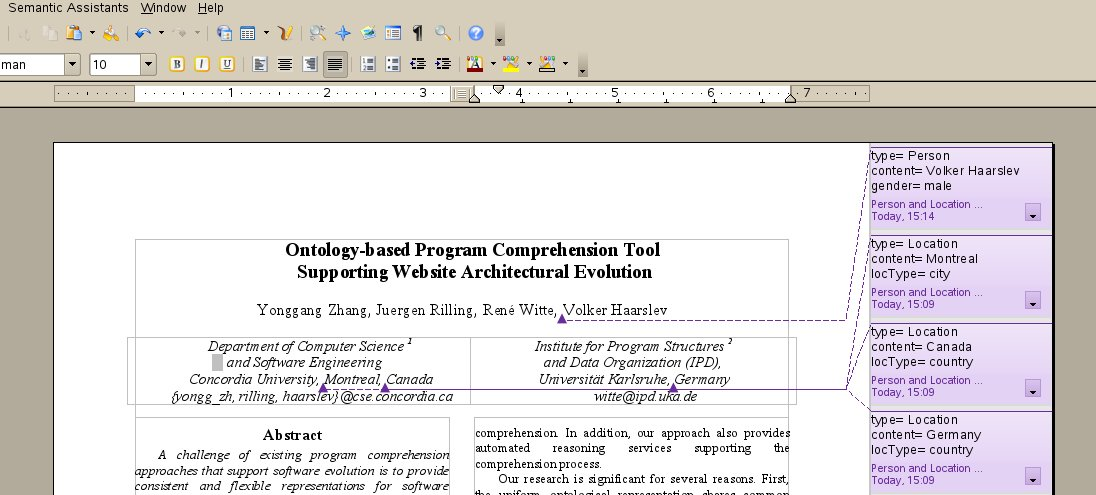
\includegraphics[width=0.8\textwidth]{pictures/sidenotes.jpg}
  \caption{Auto-Generated SideNotes Example}
  \label{fig:sidenotes}
  %\vspace*{-0.4cm}
\end{figure}

\subsection{New Document Creation}
\label{sec:doc-cre}
Creation of a new document comes handy when the output of an NLP service
corresponds to a complete document, or the result itself is indivisible. Some
examples are summarization or question-answering (see Figure~\ref{fig:oores}).

\begin{figure*}[htb]
  \centering
  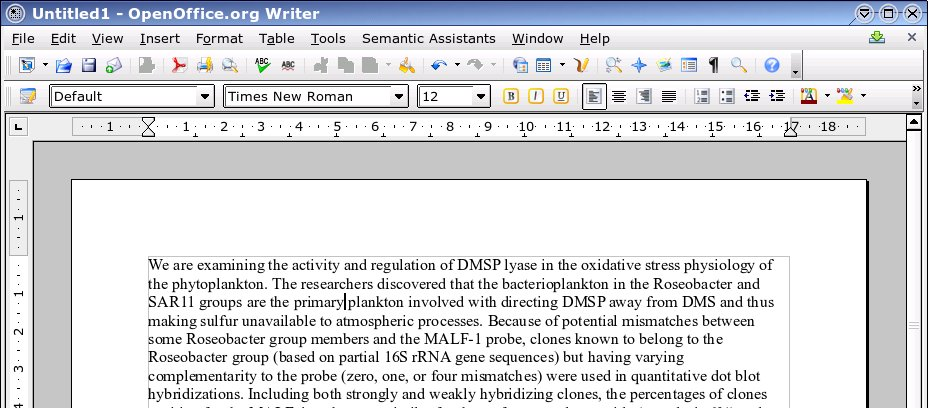
\includegraphics[width=0.8\textwidth]{pictures/ooresult_clip.jpg}
  \vspace*{-2mm}
  \caption{NLP services can also create a completely new document as a
  result (e.g., through summarization)}
  \label{fig:oores}
\end{figure*}

\subsection{Annotation Highlighting}
Besides text annotation, we offer the option for enabling/disabling annotation
highlighting for text that has been processed by GATE. This option can be
found under the Semantic Assistants menu in ``Global Settings.''  See
Figure~\ref{fig:highlight} for an example.

\subsection{Filter Empty Features}
This option found under the Semantic Assistants menu in ``Global Settings'' (shown
in Figure~\ref{fig:oosettings}) allows the ability to enable/disable filtering of
empty valued features in side-nodes. This can be useful to avoid cluttering or aid
debugging annotations respectively.

\subsection{Show Annotation Content}
This option in the ``Global Settings'' dialog can be used to include/exclude
the annotated content within the side-note. This can be used as an alternative
to annotation highlighting.

\begin{figure}
  \centering
  %\vspace*{-9mm}
  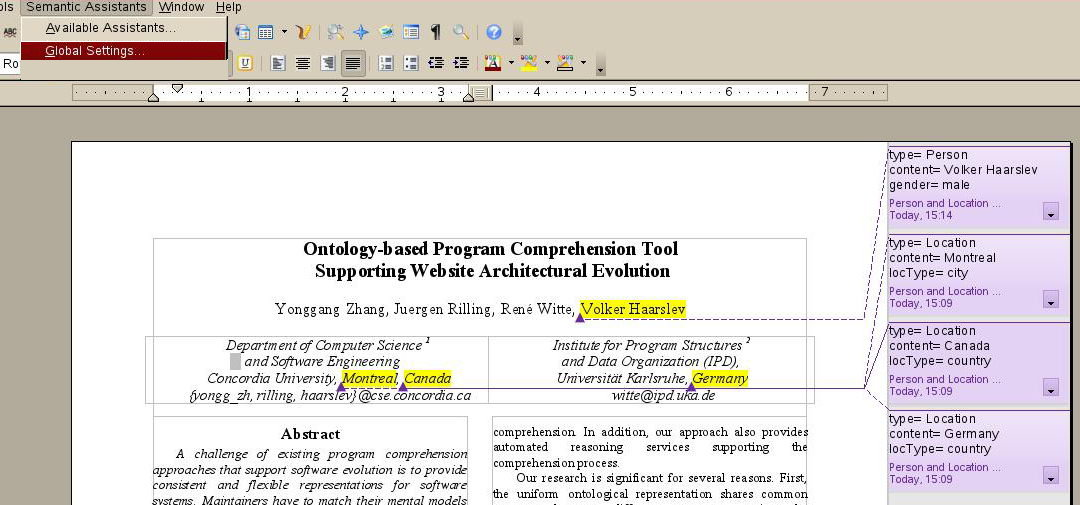
\includegraphics[width=0.8\textwidth]{pictures/highlighting.jpg}
  \caption{Highlighted Annotations Example}
  \label{fig:highlight}
  %\vspace*{0.5cm}
\end{figure}

\begin{figure}[htb]
\begin{center}
  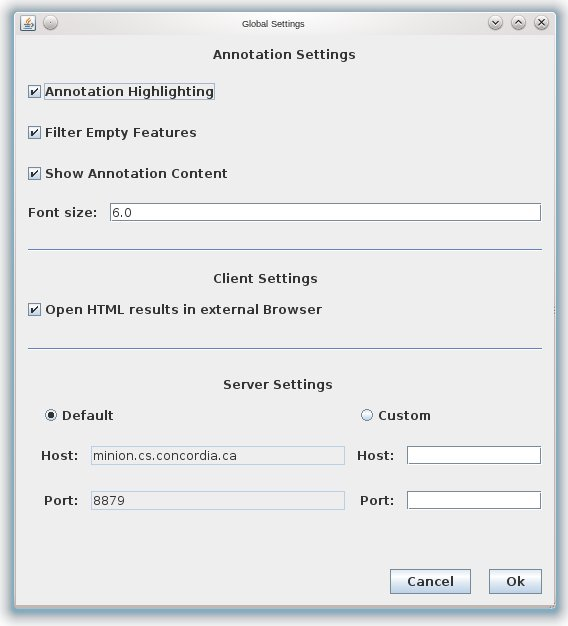
\includegraphics[width=0.5\textwidth]{pictures/oosettings.jpg}
  \caption{Configuration Dialog}
  \label{fig:oosettings}
\end{center}
\end{figure}

\subsection{Annotation Font Size}
As shown in Figure~\ref{fig:oosettings}, the font size of annotations can be changed
prior to invoking assistants. Due to the fixed width of side-notes, customizing the
size can ease readability of features.

\subsection{Browser Handling of HTML Results}
Instead of returning annotations, some pipelines produce HTML documents. The
``Open HTML results in external Browser'' option shown in Figure~\ref{fig:oosettings},
allows OpenOffice to invoke a local browser to display these results.

\subsection{Server Settings}
Another option found under the Semantic Assistants menu in ``Global
Settings.'' is \emph{Server Settings}.  There the user is able to specify the
Server information (Host and Port) of a local or distant server.

\section{Installation}
\label{subsec:oo-inst}
The OpenOffice.org plug-in can be found in
\url{SemanticAssistants/Clients/OpenOffice} and it is compatible with 
OpenOffice versions greater than 2.0.4. To use it, do the following:

\begin{enumerate}
  % TODO: what about the OO SDK installation? 
  % Is it needed for running the plug-in?

  \item Start OpenOffice.org Writer and ensure the right Java VM is
  used. Go to \emph{Tools $\rightarrow$ Options}. Under
  \emph{OpenOffice.org} you will find a \emph{Java} item. There, you
  can specify JREs. If it is not already there, add the currently used
  Java version.
  
  % should add screenshots for this
  \item Go to \emph{Tools $\rightarrow$ Extension Manager}. Click the
    \emph{Add$\ldots$} button on the bottom. Navigate to your local
    copy of the \sa\ architecture and then to
    \texttt{Clients/OpenOffice}. Select the file
    \texttt{SemassistOpenOfficePlugIn.oxt} and click \emph{Open}.

  \item Leave the dialog and open a new text document. You should have
    a new menu bar entry labeled \emph{Semantic Assistants}. Now you
    can run services on the current document (remember the server must
    be running to be able to query or execute language services).
\end{enumerate}


\section{Development Notes}
\label{sec:oo-spec}
In this section, we provide further technical details on our plug-in
for developers interesting in enhancing or modifying it.

\subsection{Compiling the Plug-in}
If you want to build the plugin yourself, follow these steps:
\begin{itemize}
  \item cd to the \url{Clients/OpenOffice} directory.

  \item Type \texttt{ant run}, or \texttt{ant run-gui}. Note that the
    client-side abstraction layer must have already been built and
    packaged. Both \texttt{ant run} and \texttt{ant run-gui} provide
    an UNO package named \url{SemassistOpenOfficePlugIn.oxt}. Both
    targets additionally copy it to \url{~/Documents/uno-components}.
    If \texttt{ant run-gui} is issued the OpenOffice.org
    \emph{Extension Manager} will pop up and prompt the user to
    install the extension.  If \texttt{ant run} is issued the above
    process is automated.  After the installation, OpenOffice Writer
    starts with the plug-in installed.

    \textbf{Note:} you can also manually add the plug-in from within
    OpenOffice (skip this step if you already used the \emph{run} or
    \emph{run-gui} target): Go to Tools, Extension Manager. Select
    \emph{My Extensions}, then click \emph{Add...} on the
    right. Choose the UNO package (available in
    \url{~/Documents/uno-components} if you used the \emph{deploy}
    target for ant).
\end{itemize}

\subsection{OpenOffice.org Plug-in Specifics}
Every plug-in has to include a \emph{description.xml} that describes the 
package's meta details like publisher, license, download url and version dependencies.
See \href{http://wiki.services.openoffice.org/wiki/Documentation/DevGuide/Extensions/Description_of_XML_Elements}{OpenOffice Developer's Guide}
for a list of available elements. The plug-in package also includes a
\emph{META-INF} directory, which contains a file called
\emph{manifest.xml}. This XML file lists the elements that come with
this plug-in;  The concrete manifest file for our plug-in is listed in
Figure~\ref{list:manifest}.  We can see that it defines three
\emph{file-entry} elements specifying the type and location of the
following files:
\begin{figure}[tb]
\centering
\begin{lstlisting}[language=XML,numbers=left,xleftmargin=8mm,columns=flexible]
<?xml version="1.0" encoding="UTF-8"?> 
<!DOCTYPE manifest:manifest PUBLIC 
"-//OpenOffice.org//DTD Manifest 1.0//EN" "Manifest.dtd"> 
<manifest:manifest 
 xmlns:manifest="http://openoffice.org/2001/manifest"> 
  <manifest:file-entry 
     manifest:media-type=
        "application/vnd.sun.star.configuration-data" 
     manifest:full-path="Addons.xcu"/> 
  <manifest:file-entry 
     manifest:media-type=
        "application/vnd.sun.star.configuration-data" 
     manifest:full-path="ProtocolHandler.xcu"/> 
  <manifest:file-entry 
     manifest:media-type=
        "application/vnd.sun.star.uno-component;type=Java" 
     manifest:full-path=
        "ProtocolHandlerAddon_java.uno.jar"/>
   <!-- Add any other plug-in required jar files here. -->
</manifest:manifest> 
\end{lstlisting}
\caption{The \emph{manifest.xml} file for our plug-in}
\label{list:manifest}
\end{figure}


\begin{description}
\item[\emph{Addons.xcu}.] This XML file defines how the plug-in should
  be integrated with OpenOffice.org. In our case, it contains a menu
  definition, specifying that the menu should only appear in the
  \emph{Writer} application. For each menu item, we specify which
  messages should be broadcast throughout the OpenOffice.org runtime
  system when the menu item is activated.
\item[\emph{ProtocolHandler.xcu}. ] This XML file specifies that the
  messages defined in \emph{Addons.xcu} should be handled by an object
  of a certain class. This class is provided in the Java archive and
  must adhere to a certain interface. 
\item[\emph{ProtocolHandlerAddon\_ java.uno.jar}.] This Java archive
  contains the actual functionality of the plug-in. It holds classes
  responsible for receiving the messages generated by the menu items,
  as well as classes responsible for the interaction with the
  client-side abstraction layer.
\end{description}


\subsection{Implementation Details}
A useful class called \url{UNOUtils} found in the \url{package
  info.semanticsoftware.semassist.client.openoffice.utils} contains most of
the OO-Writer feature implementations.  More specifically, the three methods in
Figure~\ref{list:ssb} implement a major part of the above described features
(Side-Notes, Highlighting and New Document Creation).

\begin{figure}
\centering
\begin{lstlisting}[language=Java,numbers=left,xleftmargin=8mm,columns=flexible]

private static XComponent CreateNewDocument( XDesktop xDesktop, 
					     String sDocumentType )
{
	...
}

private static void AnnotateField( Annotation annotation )
{
	...
	// Use the text document's factory to create an Annotation text field
	XTextField xAnnotation = (XTextField) UnoRuntime.queryInterface(
		XTextField.class, mxDocFactory.createInstance(
		"com.sun.star.text.TextField.Annotation" ) );
	
	// get the properties of the field
	XPropertySet xPropertySet = (XPropertySet) UnoRuntime.queryInterface( 
						XPropertySet.class, xAnnotation
);
	
	...
	
	// Highlight annotated field
        HighlightField();
}

private static void HighlightField()
{
....

}
\end{lstlisting}
\caption{Core methods implementing the OpenOffice Writer plug-in features are
  part of the \texttt{UNOUtils} class}
\label{list:ssb}
\end{figure}

%More details on how to compile and debug an OpenOffice plug-in can be found in Section~\ref{sec:debug}.
 
\subsection{Configure the OpenOffice Writer to Run in Debug Mode}
This Section describes how to configure the JAVA VM in OpenOffice Writer to accept incoming connection for a debugger.

\begin{enumerate}
  \item Open OpenOffice Writer
  \item Go to Tools, Options. Under \emph{OpenOffice.org}, there is a \emph{Java} item. Select it and then Click on the 
        \emph{Parameter} button. There the parameters when running the JAVA VM are set.
  \item To run in debug mode \emph{Assign} the following 2 parameters:
  \begin{itemize}
    \item \textbf{-X debug}
    \item \textbf{-Xrunjdwp:transport=dt\_socket,server=y,suspend=n,address=7081}
  \end{itemize}
  \item \textbf{Note: The} \emph{address=7081} \textbf{should be the consistent with the port set within the debugger}
  \item  Now OO Writer is ready to accept connections from the debugger
\end{enumerate} 

% Semantic Assistants - http://www.semanticsoftware.info/semantic-assistants
%
% This file is part of the Semantic Assistants architecture.
%
% Copyright (C) 2011, 2012, 2013 Semantic Software Lab, http://www.semanticsoftware.info
% The Semantic Assistants architecture is free software: you can
% redistribute and/or modify it under the terms of the GNU Affero General
% Public License as published by the Free Software Foundation, either
% version 3 of the License, or (at your option) any later version.
%  
% This program is distributed in the hope that it will be useful,
% but WITHOUT ANY WARRANTY; without even the implied warranty of
% MERCHANTABILITY or FITNESS FOR A PARTICULAR PURPOSE.  See the
% GNU Affero General Public License for more details.
% 
% You should have received a copy of the GNU Affero General Public License
% along with this program.  If not, see <http://www.gnu.org/licenses/>.

\chapter{Eclipse Plug-in}
Eclipse is not a single monolithic program, but rather a small kernel containing
a plug-in loader surrounded by hundreds of plug-ins. The behavior of each
plug-in in this architecture is stored in its code, and its dependencies and
services are declared in the plug-in's manifest file. On each Eclipse startup,
the plug-in loader scans all the available manifest files in the Eclipse
exclusive plug-in folder and then builds a structure containing this
information.

We used this characteristic of Eclipse architecture to integrate our Semantic
Assistants architecture into the Eclipse environment in form of a plug-in, in
order to offer various Natural Language Processing services. The Semantic
Assistants Eclipse plug-in is basically a Java archive (JAR) file that ships
with its own specific content and a description file to introduce itself to the
Eclipse plug-in loader. 

\section{Features}
Once the Semantic Assistants plug-in is installed, it creates a new menu entry
in the Eclipse menu toolbar. A user can inquire about the available services
from the ``Available Assistants'' item and modify the connection settings to the
Semantic Assistants server by selecting the second item.
\begin{figure}[htb]
\begin{center}
  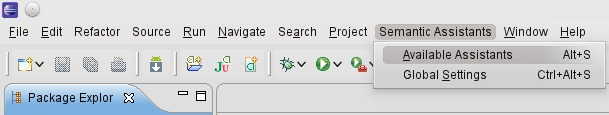
\includegraphics[width=1.0\textwidth]{pictures/eclipse_menu.jpg}
  \caption{Semantic Assistant Menu in Eclipse}
  \label{fig:eclipse_menu}
\end{center}
\end{figure}
\subsection{Available Assistants}
Selecting the ``Available Assistants'' item from Semantic Assistants menu will
open a file selection dialog. The file selection dialog allows the user to
select the desired files, folders and even complete projects to send to the
server as inputs to an NLP service. For more convenience, you can type an arbitrary extension like ``java'' or ``xml'', in the ``File Format'' field to filter to file tree view. 

\begin{figure}[htb]
\begin{center}
  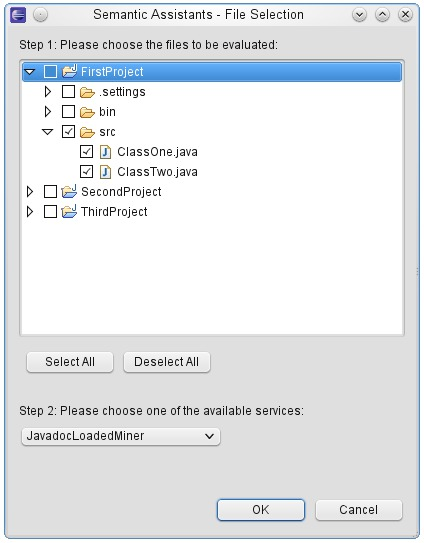
\includegraphics[width=0.5\textwidth]{pictures/eclipse_fileSelection.jpg}
  \caption{File Selection Dialog}
  \label{fig:eclipse_fileSelection}
\end{center}
\end{figure}

This dialog also lets the user to select an NLP service from a dynamically
generated list of services. This list is generated dynamically by selecting the
available services based on the client and the language capabilities of the
deployed NLP services. The server location where the service information are read from is presented just above the list as depicted in Fig \ref{fig:eclipse_services}. Note that the integration of a new service does not
require any changes on the client side - any new NLP service created and
deployed by a language engineer is dynamically discovered through its OWL
metadata maintained by the architecture and so becomes immediately available to
any connected client.

\begin{figure}[htb]
\begin{center}
  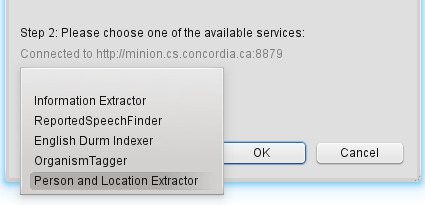
\includegraphics[width=0.5\textwidth]{pictures/eclipse_services.jpg}
  \caption{A List of Available NLP Services}
  \label{fig:eclipse_services}
\end{center}
\end{figure}

Upon selecting the resource files and the desired service, the user can execute
the selected service on the checked files in the tree. Consequently, the user will be informed about the status of the execution in the ``Semantic Assistant Status'' view. A successful execution of the selected NLP service, will let the user know on how to view the results. If the service execution fails, a description of the occurred error will be shown to the user and invocation will be aborted.

Now, let's look at how different types of outputs are handled in the plug-in:

\paragraph{Annotations.}
Annotations retrieved from a successful service invocation are being shown to the user in an
Eclipse view part called ``Semantic Assistants'' view. In the mentioned view, a
table will be dynamically generated that contains
all the parsed annotation instances. In Figure~\ref{fig:eclipse_saView} the
result of an execution of the ``Person and Location Extractor'' service on two
sample classes is shown.
\begin{figure}[htb]
\begin{center}
  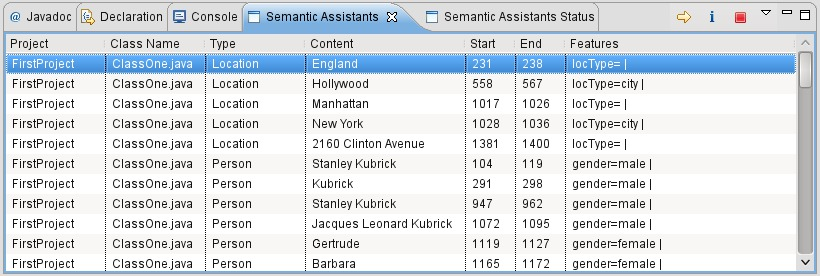
\includegraphics[width=1\textwidth]{pictures/eclipse_saView.jpg}
  \caption{Semantic Assistants View}
  \label{fig:eclipse_saView}
\end{center}
\end{figure}

This table can be sorted by different criteria through clicking on each column
title. Additionally, by double-clicking on each row in the table, the selected
annotation will appear with a graphical representation attached to the
corresponding resource. For instance, in Figure~\ref{fig:eclipse_annotation} the
JavadocMiner service has been invoked on a Java source code file. Some of the
annotations returned by the server bear a \emph{lineNumber} feature, which
attaches an annotation instance to a specific line in the java source file. Upon
double-clicking on the annotation instance in the Semantic Assistant view, the
corresponding resource - here, a .java file - will be opened in an editor and an
Eclipse warning marker will appear next to the line defined by the annotation
\emph{lineNumber} feature.

\begin{figure}[htb]
\begin{center}
  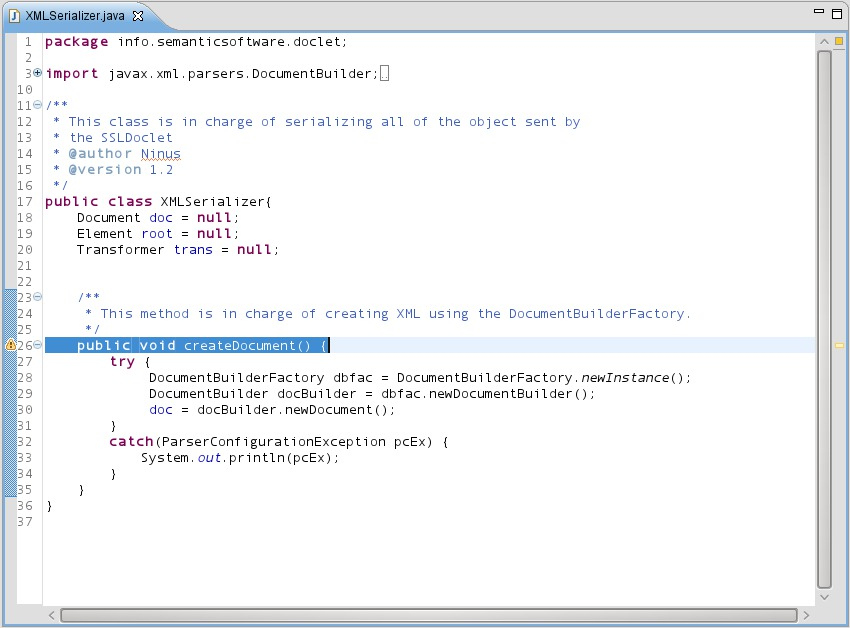
\includegraphics[width=1\textwidth]{pictures/eclipse_annotation.jpg}
  \caption{A Semantic Annotation}
  \label{fig:eclipse_annotation}
\end{center}
\end{figure}

\paragraph{Boundless Annotations.}
Boundless Annotations are a special kind of Annotations that adhere to a whole document and thus have no start and end offset. The plug-in parses the annotation results, and then inserts the content of the annotations in a new document and opens it in a new editor inside the Eclipse environment.

\paragraph{Documents.}
Documents received from the server response carry a URL property where defines where they are located. The plug-in retrieves the URLs and inserts them into a new document that opens up in a new editor inside the Eclipse environment.

\paragraph{Files.}
When a file output type is received by the plug-in, it will try to open it up in a web browser. In Eclipse, users can configure whether they want to open URLs in the Eclipse built-in web browser or any other ones in the file system. Whichever defined as the default behavior in Eclipse by the user, will be used by the plug-in to present the result file to the user. In this case, a log message will be shown to the user in the ``Semantic Assistants Status'' view to inform the user that the file is opened in his browser.

\subsection{Global Settings}
The second option found under the Semantic Assistants menu is the ``Global
Settings'' item. By clicking on this menu item, a dialog as depicted in Figure \ref{fig:eclipse_settings} is shown to the user that lets him choose a preferred server from a list of pre-defined values or add a custom server to the settings file. The values are provided in the Semantic Assistants global preference file described in \ref{sec:pref_management}. If the preference file gets accidentally deleted, a default preference file will be created by the plug-in but the eclipse-specific settings will be lost.
\begin{figure}[htb]
\begin{center}
  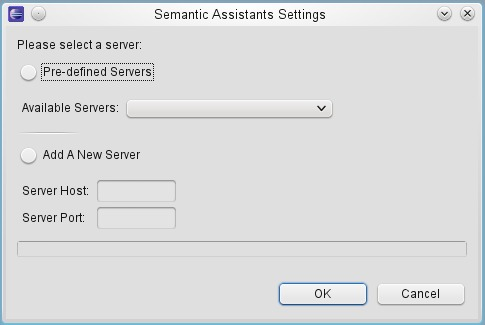
\includegraphics[width=0.6\textwidth]{pictures/eclipse_settings.jpg}
  \caption{Semantic Assistants Server Settings Dialog}
  \label{fig:eclipse_settings}
\end{center}
\end{figure}

\section{Installation}
\label{subsec:eclipse_install}
You can install the Semantic Assistants plug-in via the Eclipse software installer. To do so, first you have to add the Semantic Assistants software repository to your Eclipse list of software sites. In addition to installing the plug-in, adding the repository lets the Eclipse update manager to check for plug-in updates once available. Please carefully follow the steps listed below to install the Eclipse plug-in and refer to section \ref{trouble:eclipse_install} for installation troubleshooting.

\begin{enumerate}
  \item Select Help $\rightarrow$ Install New Software to open the Eclipse software installer.
  \item Press the ``Add'' button in the dialog, to add the Semantic Assistants repository.
  \item In the new dialog depicted in Fig \ref{fig:eclipse_install}, type ``\texttt{Semantic Assistants}'' and\\ ``\texttt{http://sa-eclipse.semanticsoftware.info}'' in ``Name'' and ``Location'' fields, respectively, and press ``OK''.
  \item The Semantic Assistants repository should now be added to your Eclipse list of software sites as seen in Fig \ref{fig:eclipse_install2}. From the loaded softwares, check the Eclipse plug-in and press ``Next''.
  \item Simply, follow the installation steps and let the installer restart the Eclipse application.
  \item The Eclipse plug-in loader will automatically load the plug-in for you. If the plug-in is installed
successfully, you should be able to see the Semantic Assistants menu added to
you toolbar.
\end{enumerate}

\begin{figure}[htb]
\begin{center}
  \includegraphics[width=0.6\textwidth]{pictures/eclipse_install.jpg}
  \caption{Adding Semantic Assistants Repository to Eclipse List of Software Sites}
  \label{fig:eclipse_install}
\end{center}
\end{figure}

\begin{figure}[htb]
\begin{center}
  \includegraphics[width=0.6\textwidth]{pictures/eclipse_install2.jpg}
  \caption{Eclipse Software Installer Dialog}
  \label{fig:eclipse_install2}
\end{center}
\end{figure}

\section{Updating The Plug-in}
\begin{enumerate}
  \item Select Help $\rightarrow$ Check for Updates to open the Eclipse update manager.
  \item If there are any updates available for the Semantic Assistants plug-in, it will appear the in the update manager dialog as shown in Fig \ref{fig:eclipse_update}.
  \item Check the Semantic Assistants Eclipse plug-in from the list and press ``Next''.
  \item Follow the wizard steps and let the update manager restart your Eclipse for the updates to take place.
\end{enumerate}

\begin{figure}[htb]
\begin{center}
  \includegraphics[width=1.0\textwidth]{pictures/eclipse_update.jpg}
  \caption{Updatin the Plug-in via Eclipse Update Manager}
  \label{fig:eclipse_update}
\end{center}
\end{figure}

\section{Development Notes}
\label{subsec:eclipse.development}
In this section, we provide further technical details on our plug-in for
developers interesting in enhancing or modifying it.

\subsection{Plug-in Source Directory Structure}
The Semantic Assistants plug-in uses Model-View-Controller pattern for its
implementation. Thus, most of the source code files are divided into different
packages related to their responsibilities. When you browse to
\url{src/info/semanticsoftware/semassist/client/eclipse/} folder, you see the
following structure:
\begin{enumerate}
\item\url{dialogs}: This folder contains the dialogs that are shown to the user
for interactions e.g. file selection. The classes inside this folder are the
codes for graphical user interfaces.
\item\url{handlers}: This folder contains the classes which play the controller
role in MVC pattern. Examples of these classes are dialog handlers and service
invocation jobs.
\item\url{model}: This folder contains the classes that provide data for
graphical user interfaces. These models are consumed by classes inside
\texttt{views} package.
\item\url{utils}: This folder contains utility classes e.g. logging feature.
\item\url{views}: This folder contains the source codes for Semantic Assistants
view parts. These are again graphical user interfaces but packaged differently
from dialogs.
\end{enumerate}

There is also another file called \url{Activator.java} in the source directory.
It is the main class of the plug-in that will be loaded initially and control
the plug-in's life cycle.

\subsection{Modifying the Plug-in}
If you want to modify the plug-in behavior or enhance it, follow these steps:
\begin{enumerate}
\item Open the Eclipse application.
\item Select File $\rightarrow$ New  $\rightarrow$ Project and under the
``Plug-in Development'' category select the ``Plug-in Project''.
\item A new plug-in project wizard will open up. Keep the EclipsePlugin name for
the project. Just below the project name there is a checkbox reading ``Use
Default Location''. Uncheck it and browse to the EclipsePlugin folder inside
where you've stored the Semantic Assistants folder.
\item Leave the other options untouched and press Finish.
\end{enumerate}

\begin{figure}[htb]
\begin{center}
  \includegraphics[width=0.5\textwidth]{pictures/eclipse_project_wizard.jpg}
  \caption{Eclipse New Plug-in Project Wizard}
  \label{fig:eclipse_project_wizard}
\end{center}
\end{figure}

\textbf{Note:} Remember you should manually copy the CSAL.jar file into you the
project's \texttt{lib} folder because it is a part of the project's dependency
and is defined in the classpath.

When the project is loaded in your workspace, feel free to play around. Browse
the source directory and add your development codes. To run your code, right
click on \texttt{plugin.xml} file and select Run As $\rightarrow$ Eclipse
Application.

%% Semantic Assistants - http://www.semanticsoftware.info/semantic-assistants
%
% This file is part of the Semantic Assistants architecture.
%
% Copyright (C) 2009, 2010, 2011 Semantic Software Lab, http://www.semanticsoftware.info
% The Semantic Assistants architecture is free software: you can
% redistribute and/or modify it under the terms of the GNU Affero General
% Public License as published by the Free Software Foundation, either
% version 3 of the License, or (at your option) any later version.
%   
% This program is distributed in the hope that it will be useful,
% but WITHOUT ANY WARRANTY; without even the implied warranty of
% MERCHANTABILITY or FITNESS FOR A PARTICULAR PURPOSE.  See the
% GNU Affero General Public License for more details.
% 
% You should have received a copy of the GNU Affero General Public License
% along with this program.  If not, see <http://www.gnu.org/licenses/>.

\chapter{Extension for Mozilla Firefox and Mozilla Thunderbird} 

The Mozilla extension allows users to use Semantic Assistants in Mozilla Firefox and Mozilla Thunderbird and to leverage the \sa architecture within those applications. It is built on the extension platform that shared by Mozilla Firefox and Mozilla Thunderbird. Hence, it is a single extension that is compatible with both applications. The Mozilla extension aims to take the capabilities provided by Semantic Assistants and integrate them within the workflow of web browsing and of email reading and management. 

\section{Features}
\label{subsec:mozilla_features}

\subsection{User Interface Elements}
When the \sa Mozilla extension is installed, some new UI elements are added to the interface of the application. Firstly, a new ``Semantic Assistants" menu is added on the menu bar. Secondly, a new toolbar button is added to the primary toolbar of the application. (This toolbar button may be removed or relocated using Firefox/Thunderbird's built-in customization capabilities.) The toolbar button is actually a ``menu button," i.e., the left part is a button, and the right part opens a menu when clicked. Thirdly, a menu item is added to the contextual (right-click) menu of the principal content area of the application, that is, the browsing area in Firefox and the message body pane in Thunderbird. Lastly, a sidebar, which can be opened and closed, is added to the main window of the application. 

\paragraph{The ``Semantic Assistants" menu.} The ``Semantic Assistants" menu is 
located on the menu bar and opens a menu with the following three menu items: 
\begin{itemize} 
  \item Available Assistants... 
  \item Semantic Assistants Sidebar 
  \item Global Settings... 
\end{itemize} 

The ``Semantic Assistants" menu is shown in Figure~\ref{fig:mozilla_features_toolbar_menu_button}. 

\begin{figure}[htb]
  \centering
  \includegraphics[width=0.8\textwidth]{pictures/mozilla_features_toolbar_menu_button.png}
  \caption{The toolbar menu button in Firefox and Thunderbird}
  \label{fig:mozilla_features_toolbar_menu_button}
\end{figure}

\paragraph{The ``Available Assistants" toolbar menu button.} The ``Available Assistants" menu button is located on the toolbar. The left side is a button and executes the ``Available Assistants" command (further elaborated later). Clicking the right side opens a menu that is identical to the ``Semantic Assistants" menu. 

\paragraph{The ``Available Assistants..." contextual menu item.} The ``Available Assistants" menu item appears on the contextual (right-click) menu of the main browsing area/page content area in Firefox and in the message body area in Thunderbird. Like the toolbar button, it also invokes the ``Available Assistants" command. 

\paragraph{The ``Semantic Assistants Sidebar".} The ``Semantic Assistants Sidebar" appears on the left side of the main window in Firefox and on the right side of the main window in Thunderbird. (The discrepancy is explained as follows. Firefox has built-in support for adding sidebars, and these appear on the left side of the main browsing window. Thunderbird, on the other hand, has no sidebars. Furthermore, the main inbox tab in Thunderbird already has a folder pane on the left side of the window. Hence, a custom sidebar was added, and it was placed on the right side of the main window.) 

The ``Semantic Assistants Sidebar" displays the results obtained from a service invocation to a Semantic Assistant. The following button in the Sidebar operate on the results: 
\begin{itemize} 
  \item \emph{Expand all}: Expands nodes of the results tree by one level.
  \item \emph{Collapse all}: Collapses all nodes of the results tree.
  \item \emph{Underline all}: Underlines all results in the tree in the page/message.
  \item \emph{Underline none}: Clears all the underlining in the page/message.
  \item \emph{Find previous underlined item}: Selects (highlights) the previous underlined text in the page/message.
  \item \emph{Find next underlined item}: Selects (highlights) the next underlined text in the page/message.
\end{itemize} 
The ``Semantic Assistants Sidebar" can be opened using the following ways: 
\begin{itemize} 
  \item \emph{Semantic Assistants} menu $\rightarrow$ \emph{Semantic Assistants Sidebar}
  \item \emph{Available Assistants} toolbar button menu $\rightarrow$ \emph{Semantic Assistants Sidebar}
  \item (in Firefox) \emph{View} menu $\rightarrow$ \emph{Sidebar} $\rightarrow$ \emph{Semantic Assistants Sidebar}
  \item (in Thunderbird) \emph{View} menu $\rightarrow$ \emph{Layout} $\rightarrow$ \emph{Semantic Assistants Sidebar}
  \item the keyboard shortcut \emph{Ctrl Shift S}
\end{itemize} 

The ``Semantic Assistants Sidebar" dialog is shown in Figure~\ref{fig:mozilla_features_sidebar}. 

\begin{figure}[htb]
  \centering
  % \includegraphics[width=0.8\textwidth]
  \includegraphics[totalheight=0.5\textheight]{pictures/mozilla_features_sidebar.png}
  \caption{The ``Semantic Assistants Sidebar" in Firefox and Thunderbird}
  \label{fig:mozilla_features_sidebar}
\end{figure}

\paragraph{The ``Global Settings" dialog.} The ``Global Settings" dialog allows the user to configure certain settings for the extension. These settings include:
\begin{itemize} 
  \item \emph{Server settings}: The user may choose to use the default defined server or to specify a custom server address. 
  \item \emph{Script settings}: The processing of the results is handled by a script run in Firefox/Thunderbird. If there are a lot of results or the page/message is long, the script may run for a long time. Firefox/Thunderbird has the built-in capability to prompt the user when a script has run for a given amount of time. By default, this amount of time is 20 seconds. The user may change this period if desired. Setting this setting to 0 signifies that the script will run forever. (Doing so, however, is not recommended, as the script may run for a very long time, and the only way to cancel would be to kill the whole application.)
\end{itemize} 
The ``Global Settings" dialog can be opened using the following ways: 
\begin{itemize} 
  \item \emph{Semantic Assistants} menu $\rightarrow$ \emph{Global Settings...}
  \item \emph{Available Assistants} toolbar button menu $\rightarrow$ \emph{Global Settings...}
\end{itemize} 

The ``Global Settings" dialog is shown in Figure~\ref{fig:mozilla_features_global_settings}. 

\begin{figure}[htb]
  \centering
  \includegraphics[width=0.8\textwidth]{pictures/mozilla_features_global_settings.png}
  \caption{The ``Global Settings" dialog in Firefox and Thunderbird}
  \label{fig:mozilla_features_global_settings}
\end{figure}

\subsection{Invoking a Semantic Assistant}
When the ``Available Assistants" command is invoked (either using the menu item in the ``Semantic Assistants" menu or in the menu of the toolbar button), a dialog entitled ``Available Semantic Assistants Services" appears (shown in Figure~\ref{fig:mozilla_features_available_assistants_dialog}), listing all available services from the server along with descriptions of each service. Upon the selection of a service, the extension sends the user-selected text in the page/message or, if text no selection was made, the whole text content of the page/message.

\begin{figure}[htb]
  \centering
  \includegraphics[width=1\textwidth]{pictures/mozilla_features_available_assistants_dialog.png}
  \caption{The ``Available Semantic Assistants Services" dialog in Firefox and Thunderbird}
  \label{fig:mozilla_features_available_assistants_dialog}
\end{figure}

When the results are returned by the server, two things happen. Firstly, the results are underlined in the page/message directly in the browsing area/message content area. Secondly, the ``Semantic Assistants Sidebar" is opened if it is not already so and displays the results. 

\subsection{Viewing the Results}
The results from the service invocation are underlined directly in the content of the page/message. The underlining is color-coded by annotation type to allow for better visual distinction. 

The results are also displayed in the ``Semantic Assistants Sidebar" in a tree format, grouped by annotation type, then by occurrences of a same word/phrase. 

The controls/buttons in the ``Semantic Assistants Sidebar" (mentioned previously in the ``User Interface Elements" section) can be used to manipulate the results tree, to underline all or no results and to go to the previous/next underlined result in the page/message.

Clicking on a node in the results tree will underline in the page/message the result or results represented by the node and all children of the node. For instance, if a leaf node of the tree is clicked in the Sidebar, the one result represented by that node is underlined. If an inner node of the tree is clicked in the Sidebar, then all the results represented by that node and all its child nodes are underlined. The ``Find previous underlined item" and ``Find next underlined item" buttons in the Sidebar will navigate only the currently underlined results. All put together, this allows to display precise subsets of the results, and to navigate through the occurrences of these results. 

The display of results within Firefox and Thunderbird is shown in Figure~\ref{fig:mozilla_features_firefox_window} and Figure~\ref{fig:mozilla_features_thunderbird_window_message_tab}.

\begin{figure}[htb]
  \centering
  \includegraphics[width=0.95\textwidth]{pictures/mozilla_features_firefox_window.png}
  \caption{Results from a service invocation in Firefox}
  \label{fig:mozilla_features_firefox_window}
\end{figure}

\begin{figure}[htb]
  \centering
  \includegraphics[width=0.95\textwidth]{pictures/mozilla_features_thunderbird_window_message_tab.png}
  \caption{Results from a service invocation in Thunderbird}
  \label{fig:mozilla_features_thunderbird_window_message_tab}
\end{figure}

\section{Installation}
\label{subsec:mozilla_installation}
The Mozilla extension comes in the form of a file with a .xpi extension. The .xpi file is installed in the standard manner in which extensions are installed in Mozilla Firefox and Mozilla Thunderbird. 

\subsection{Additional Notes about Prerequisites}
In addition to the basic prerequisites (refer to Chapter~\ref{chap:inst}), the following considerations should be noted: 
\begin{itemize}
  \item The Java runtime environment \emph{must} be the official Java Development Kit from Oracle (formerly from Sun). In certain Linux installations, OpenJDK is installed by default. This will not work for the Mozilla extension. (A ``java is not defined" error will occur.)
\end{itemize}

\subsection{Installation in Mozilla Firefox}
There are two methods to install the .xpi file in Firefox. The first method is to drag and drop the .xpi file into Firefox.
\begin{enumerate}
  \item Drag and drop the .xpi file into the main browsing area of the Firefox window.
  \item A dialog window entitled "Software Installation" appears. Click the ``Install Now'' button in the dialog.
  \item Restart Firefox.
\end{enumerate}
An alternate method is to use the file picker in Firefox.
\begin{enumerate}
  \item Select \emph{File $\rightarrow$ Open File...}.
  \item Navigate to the location of the .xpi file and choose it.
  \item A dialog window entitled "Software Installation" appears. Click the ``Install Now'' button in the dialog.
  \item Restart Firefox.
\end{enumerate}

\subsection{Installation in Mozilla Thunderbird 3.1.x and earlier}
Here is how to install the .xpi file in Thunderbird version 3.1.x and earlier. 
\begin{enumerate}
  \item Select \emph{Tools $\rightarrow$ Add-ons}.
  \item The Add-ons dialog opens. In the ``Extensions" section, at the bottom left, there is a button ``Install...". Click this button.
  \item Navigate to the location of the .xpi file and choose it.
  \item A dialog window entitled "Software Installation" appears. Click the ``Install Now'' button in the dialog.
  \item Restart Thunderbird.
\end{enumerate}

\subsection{Installation in Mozilla Thunderbird 5.0 and later}
Here is how to install the .xpi file in Thunderbird version 5.0 and later. 
\begin{enumerate}
  \item Select \emph{Tools $\rightarrow$ Add-ons}.
  \item The Add-on Manager opens. Near the top right, there is a button ``Tools for all add-ons" with a cog icon. Click this button.
  \item Click the ``Install Add-on from File" menu item.
  \item Navigate to the location of the .xpi file and choose it.
  \item A dialog window entitled "Software Installation" appears. Click the ``Install Now'' button in the dialog.
  \item Restart Thunderbird.
\end{enumerate}

If the installation succeeded, after the application restarts, the ``Semantic Assistants" menu in the menu bar should be visible, and the ``Available Assistants" toolbar button should be added to the toolbar. (For a full list of the UI elements of the extension, refer to section ~\ref{subsec:mozilla_features}.)

\section{Development Notes}
\label{subsec:mozilla_development}
This section details the layout of files in the extension, the overall architecture of the extension, and some specifics relating to Mozilla extension development. 

\subsection{A Brief Explanation of Mozilla Extensions}
An extension for the Mozilla platform is initially packaged in a .xpi file, which is simply a .zip file with the ``.xpi" file extension. Once the extension is ``installed" by the user, the contents of the .xpi file is extracted and placed in a newly created folder located in the ``extensions" folder within the Firefox/Thunderbird user profile folder. 

After the application restarts, the extension is loaded into memory, the installation of the extension to that specific user profile is complete.  

The Firefox/Thunderbird user profile folder is located at: 
\begin{itemize}
  \item Firefox \begin{itemize}
    \item On Windows XP: C:\textbackslash Documents and Settings\textbackslash WINDOWS\_ACCOUNT\_USER\_NAME \textbackslash Application Data\textbackslash Mozilla\textbackslash Firefox\textbackslash Profiles\textbackslash PROFILE\_FOLDER\_NAME
    \item On Windows Vista, 7: C:\textbackslash Users\textbackslash WINDOWS\_ACCOUNT\_USER\_NAME\textbackslash AppData\textbackslash Roaming \textbackslash Mozilla\textbackslash Firefox\textbackslash Profiles\textbackslash PROFILE\_FOLDER\_NAME
    \item On Linux: {\raise.17ex\hbox{$\scriptstyle\sim$}}/.mozilla/firefox/PROFILE\_FOLDER\_NAME
  \end{itemize}
  \item Thunderbird \begin{itemize}
    \item On Windows XP: C:\textbackslash Documents and Settings\textbackslash WINDOWS\_ACCOUNT\_USER\_NAME \textbackslash Application Data\textbackslash Thunderbird\textbackslash Profiles\textbackslash PROFILE\_FOLDER\_NAME
    \item On Windows Vista, 7: C:\textbackslash Users\textbackslash WINDOWS\_ACCOUNT\_USER\_NAME\textbackslash AppData\textbackslash Roaming \textbackslash Thunderbird\textbackslash Profiles\textbackslash PROFILE\_FOLDER\_NAME
    \item On Linux: {\raise.17ex\hbox{$\scriptstyle\sim$}}/.thunderbird/PROFILE\_FOLDER\_NAME or \char`\~/.mozilla-thunderbird/ PROFILE\_FOLDER\_NAME
  \end{itemize}
\end{itemize}
The profile's folder name (PROFILE\_FOLDER\_NAME) is by default a string of random characters followed by ``.default". If additional profiles are created, or if profiles are created manually, the name may be different. 

The user preferences of the extension are stored in a file called ``prefs.js" in the user profile folder. Conveniently, they can also be viewed and modified as follows. 
\begin{itemize}
  \item Firefox \begin{itemize}
    \item Type ``about:config" in the Location Bar and type Enter.
    \item If a warning message appears, click the button to continue.
  \end{itemize}
  \item Thunderbird \begin{itemize}
    \item Select \emph{Tools $\rightarrow$ Options...}.
    \item The Options dialog opens. In the ``Advanced" section, there is a button ``Config Editor...". Click this button.
    \item If a warning message appears, click the button to continue.
  \end{itemize}
\end{itemize}
A very long list of built-in Firefox/Thunderbird preferences and extension preferences is displayed. The preference in question can either be found manually, or the Filter at the top can be used to narrow down the list. Preferences can be modified by double-clicking on them. If it is a ``boolean" preference, its value is toggled. If it is a ``string" or ``integer" preference, a dialog box appears to allow the modification of the value. Changes are applied immediately. 

\subsection{File Layout}
The following covers the layout of the files of the extension. Inevitably, it will also include a brief overview of the general way a Mozilla extension works. The overall file layout can be seen in Figure~\ref{fig:mozilla_development_notes_file_layout}.

\begin{figure}[htb]
  \centering
  % \includegraphics[width=0.8\textwidth]
  \includegraphics[totalheight=0.8\textheight]{pictures/mozilla_development_notes_file_layout.png}
  \caption{The file layout of the Mozilla extension}
  \label{fig:mozilla_development_notes_file_layout}
\end{figure}

\paragraph{Root folder} At the root of extension folder are two files called ``chrome.manifest" and ``install.rdf". The ``chrome.manifest" identifies the files contained within the extension and also allows to specify which files of the extension are to be loaded, depending on the application and the version of the application on which the extension is running (more on this later). The ``install.rdf" file defines various information about the extension, including the name of the extension (which becomes the name of the aforementioned extension folder), which applications and application versions that the extension is compatible with, and so on. 
\paragraph{The ``content" folder} This contains a series of XUL (.xul) files and JavaScript (.js) files. The XUL files define the user interface elements and behavior, such as windows, dialogs, menus, toolbar buttons. The JavaScript files contain the execution logic, and manipulation of user interface elements. 
\paragraph{The ``defaults" folder} Within the ``defaults" folder is the ``preferences" folder, which contains the default preferences for the extension. Upon installation of the extension, these defaults are set as the preferences in the Firefox/Thunderbird user profile (see above for specifics about preferences). 
\paragraph{The ``java" folder} The ``java" folder contains precompiled Java classes contained within .jar files. The ``CSAL.jar" is the same Client Side Abstraction Layer found in other clients. The ``javaFirefoxExtensionUtils.jar" file is a third-party utility which allows to grant full privileges to Java within a Mozilla extension. The ``SAController.jar" file is the Java component of the extension, which acts as a bridge between the JavaScript code and the CSAL and contains some additional execution logic. 
\paragraph{The ``locale" folder} The purpose of the ``locale" folder is to contain folders that contain files with localized strings used within the extension. These folders are named by specific languages' abbreviations (e.g., ``en-US"). 
\paragraph{The ``skin" folder} The ``skin" folder contains .css files that define layout and appearance properties image resource files for the icons and various UI elements within the extension.

\subsection{Compatibility Concerns}
There are differences in the extension between Firefox and Thunderbird. Furthermore, such differences also exist between Firefox 3.6.x and Firefox 4.0 as well as between Thunderbird 3.1.x and Thunderbird 5.0. (There was no Thunderbird 4.0.) This was because major changes were made to the Mozilla platform between those versions of the appliations. 

In order to enable the extension to be compatible with multiple version of Firefox as well as multiple versions of Thunderbird, certain measures were taken. 

Files of the extensions were split such that common code between applications/versions are kept within common files, while code that is different between applications/versions are separated into different versions of the files. The appropriate set of files is loaded for the right application and version. 

The aforementioned ``chrome.manifest" file, located at the root of the extension's folder structure, specifies the files to be loaded for the extension, depending on the application and application version on which the extension is running. Hence, for example, this allows for one file to be loaded for Firefox and another file to be loaded for Thunderbird. Another example would be for one file to be loaded for Firefox version 3.6 and earlier and another file to be loaded for Firefox version 4 and later. 

The files that need to have multiple versions are both the JavaScript files and the XUL files. The JavaScript code may differ between applications/versions due to differences in API. XUL files differ between applications (less for between versions of the same application) due to differences in the user interfaces (different elements, different naming, etc.).

Table~\ref{tab:mozilla_development_files_compatibility} shows which files are used depending on the application and the version of the application. 

\begin{table}[htb]
  \centering\small\sffamily
  \begin{tabular}{p{0.5\textwidth}@{\hspace*{4mm}}p{0.08\textwidth}@{\hspace*{4mm}}p{0.08\textwidth}@{\hspace*{4mm}}p{0.08\textwidth}@{\hspace*{4mm}}p{0.08\textwidth}}
    \toprule
    \textbf{} & \textbf{Fx 3.6.x} & \textbf{Fx 4.0+} & \textbf{Tb 3.1.x} & \textbf{Tb 5.0+} \\
    \midrule
    SAOverlay.js & x & x & x & x \\

    SAOverlayHelper-fx.js & x & x &  &  \\

    SAOverlayHelper-tb.js &  &  & x & x \\

    SAOverlayExtensionLocationHelper-fx3-tb3.js & x &  & x &  \\

    SAOverlayExtensionLocationHelper-fx4-tb5.js &  & x &  & x \\

    SAOverlay-common.xul & x & x & x & x \\

    SAOverlay-fxCommon.xul & x & x &  &  \\

    SAOverlay-tbCommon.xul &  &  & x & x \\

    SAOverlay-fx3-tb3.xul & x &  & x &  \\

    SAOverlay-fx4-tb5.xul &  & x &  & x \\

    SASidebarXUL.xul & x & x & x & x \\

    SASidebarOverlay-fx.xul & x & x &  &  \\

    SASidebarOverlay-tb.xul &  &  & x & x \\
    \bottomrule
  \end{tabular}
  \caption{Files loaded depending on application and version for compatibility}
  \label{tab:mozilla_development_files_compatibility}
\end{table}

\subsection{Extension Preferences}
The default preferences of the extension are defined in the folder ``defaults" in the ``preferences" subfolder in the file ``semanticAssistants.js". As previously mentioned, the current settings of those preferences are stored in a file called ``prefs.js" in the user profile folder. 

The preferences are: 

\begin{itemize}
  \item \emph{extensions.semanticAssistants.firstTimeRun} \begin{itemize}
    \item type: boolean
    \item default value: true
    \item This determines whether it is the first time that the extension is launched. If so, it adds the toolbar menu button to the application's main toolbar. 
  \end{itemize}
  \item \emph{extensions.semanticAssistants.installLocation} \begin{itemize}
    \item type: string
    \item default value: ""
    \item This stores the path of the extension. This is not a user preference; it is utilized internally when accessing the .jar files. It is set in the extension when the application's start up. 
  \end{itemize}
  \item \emph{extensions.semanticAssistants.serverCustomHost} \begin{itemize}
    \item type: string
    \item default value: ""
    \item This is a setting set by the user in the ``Global Settings" dialog. 
  \end{itemize}
  \item \emph{extensions.semanticAssistants.serverCustomPort} \begin{itemize}
    \item type: string
    \item default value: "8879"
    \item This is a setting set by the user in the ``Global Settings" dialog. 
  \end{itemize}
  \item \emph{extensions.semanticAssistants.serverDefaultOrCustom} \begin{itemize}
    \item type: integer
    \item default value: 0
    \item 0 for ``Default", 1 for ``Custom"
    \item This is a setting set by the user in the ``Global Settings" dialog. 
  \end{itemize}
\end{itemize}

\subsection{Overall Architecture}
The Mozilla extension is composed of three components: the principal component in JavaScript and XUL, the Java component of the extension (contained in the aforementioned ``SAController.jar" file), and the Client Side Abstraction Layer/CSAL (the ``CSAL.jar" file). A high-level representation of the overall architecture is shown in Figure~\ref{fig:mozilla_development_notes_overall_architecture_high_level}).
The main part of the extension is in JavaScript and XUL, as extensions for the Mozilla platform are written in JavaScript code, and the user interface is defined in XUL. A Java component exists in order for the JavaScript component to interoperate with the CSAL; it also adds additional execution logic, such as processing the results from the CSAL. Leveraging a feature in Firefox/Thunderbird called LiveConnect in addition to a third-party package to grant full privileges to Java within a Mozilla extension, the JavaScript code of the extension utilizes and calls the compiled Java code, which in turn utilizes and calls the CSAL. 

\begin{figure}[htb]
  \centering
  \includegraphics[width=0.8\textwidth]{pictures/mozilla_development_notes_overall_architecture_high_level.png}
  \caption{The overall architecture of the Mozilla extension at a high level}
  \label{fig:mozilla_development_notes_overall_architecture_high_level}
\end{figure}

The main class in the Mozilla extension component is ``SAOverlay" (defined in ``SAOverlay.js" under the ``contents" folder). This class communicates with the other classes in the component. Additionally, it is this class that calls the Java component. The facade for the Java component is the ``SemanticAssistantsController" class. Similarly, the ``SemanticAssistantsController" class is a controller, which coordinates the other classes in the Java component. The various classes of the Java component utilize classes contained within the CSAL. These dependencies are shown in Figure~\ref{fig:mozilla_development_notes_overall_architecture_more_detailed}.

\begin{figure}[htb]
  \centering
  \includegraphics[width=0.8\textwidth]{pictures/mozilla_development_notes_overall_architecture_more_detailed.png}
  \caption{The overall architecture of the Mozilla extension showing some more details in terms of dependencies and showing some of the main modules}
  \label{fig:mozilla_development_notes_overall_architecture_more_detailed}
\end{figure}

\subsection{Main Mozilla Extension Component}
The main component of the Mozilla extension consists of a series of JavaScript classes and XUL files. The class diagram in Figure~\ref{fig:mozilla_development_notes_mozilla_extension_class_diagram} shows the main classes and their associations in the main Mozilla extension component as well as the classes called within the Java component. 

\begin{figure}[htb]
  \centering
  \includegraphics[width=0.95\textwidth]{pictures/mozilla_development_notes_mozilla_extension_class_diagram.png}
  \caption{Class diagram of the main Mozilla extension component}
  \label{fig:mozilla_development_notes_mozilla_extension_class_diagram}
\end{figure}

The main class is ``SAOverlay". When the user invokes the ``Available Assistants" command, it invokes the ``onMenuItemCommand" function in ``SAOverlay". This function obtains the user selection on the page/message, or the whole content of the page/message if no selection was made, and calls the function ``callJava" and passes the user selection. The ``callJava" function then obtains references to the Java classes in the Java component (``SAController.jar"). This is done using the feature called LiveConnect built into Firefox and Thunderbird. Additionally, the aforementioned third-party component ``javaFirefoxExtensionUtils.jar" is required to grant full privileges to the .jar files, as shown in Figure~\ref{list:mozilla_development_notes_main_mozilla_extension_component_jar_permissions}. The method ``startSemanticAssistants" of the ``SemanticAssistantsController" Java class is invoked, and the result returned is a list of available \sa NLP services (``Assistants"). Then, an XUL dialog ``SAAvailableAssistants.xul" is opened, prompting the user to choose an Assistant from the list. 

\begin{figure}
\centering
\begin{lstlisting}[language=Java,numbers=left,xleftmargin=4mm,columns=flexible]
callJava: function(userSelection, allText) {
    var extensionPath = SAOverlay.getExtensionLocation();
    
    var SAControllerJarPath = "file:///" + extensionPath + "/java/SAController.jar"; 
    var classLoaderJarPath = "file:///" + extensionPath + "/java/javaFirefoxExtensionUtils.jar";
    var CSALJarPath = "file:///" + extensionPath + "/java/CSAL.jar";
    
    urlArray = []; 
    urlArray[0] = new java.net.URL(SAControllerJarPath); 
    urlArray[1] = new java.net.URL(classLoaderJarPath);  
    urlArray[2] = new java.net.URL(CSALJarPath);  

    var cl = java.net.URLClassLoader.newInstance(urlArray);

    //set security policies with the policyAdd function defined below
    this.policyAdd(cl, urlArray);
    
    (...)
}, 

(...)

policyAdd: function(loader, urls) {
    try {
        var str = 'edu.mit.simile.javaFirefoxExtensionUtils.URLSetPolicy';
        var policyClass = java.lang.Class.forName(
            str,
            true,
            loader
            );
        var policy = policyClass.newInstance();
        policy.setOuterPolicy(java.security.Policy.getPolicy());
        java.security.Policy.setPolicy(policy);
        policy.addPermission(new java.security.AllPermission());
        for (var j = 0; j < urls.length; j++) {
            policy.addURL(urls[j]);
        }
    }
    catch(e) {
        alert(e+'::'+e.lineNumber);
    }
}
\end{lstlisting}
\caption{Granting full permissions to .jar files inside the extension in the \texttt{callJava} function in the \texttt{SAOverlay} class}
\label{list:mozilla_development_notes_main_mozilla_extension_component_jar_permissions}
\end{figure}

When the selection is made, another method ``invokeServiceAtIndex" of the ``SemanticAssistantsController" Java class is invoked, and upon successful return of the results, the ``getResults" method of the Java class is called to retrieve the results from the service invocation. Then, for each result within the results, an appropriate action is taken. For an ``annotation"-type result, the function ``underlineText" of the ``SAUnderline" JavaScript class is called; for a ``document"-type result, the function ``addURLnode" of ``SAUnderline" is called; for a ``file"-type result, no action is taken, as the Java code executes the opening the file. Save for a ``file"-type result, the ``Semantic Assistants" sidebar, which is the XUL file ``SASidebarXUL.xul", is opened to display the results. 

The sequence diagram in Figure~\ref{fig:mozilla_development_notes_mozilla_extension_sequence_diagram_main_scenario} shows the call sequence involved in the above main scenario of listing the available services and then of invoking a service. 
\begin{figure}[htb]
  \centering
  \includegraphics[totalheight=0.8\textheight]{pictures/mozilla_development_notes_mozilla_extension_sequence_diagram_main_scenario.png}
  \caption{Sequence diagram of the main Mozilla extension component for the main scenario}
  \label{fig:mozilla_development_notes_mozilla_extension_sequence_diagram_main_scenario}
\end{figure}

\subsection{Java Component}
The Java component consists of a series of Java classes packaged within a .jar file. The class diagram in Figure~\ref{fig:mozilla_development_notes_java_component_class_diagram} shows the principal classes and their associations in the Java component as well as some of the classes in the CSAL called from the Java component. 

\begin{figure}[htb]
  \centering
  \includegraphics[width=0.95\textwidth]{pictures/mozilla_development_notes_java_component_class_diagram.png}
  \caption{Class diagram of the Java component}
  \label{fig:mozilla_development_notes_java_component_class_diagram}
\end{figure}

The main class is ``SemanticAssistantsController"; it is the facade class of the Java component packaged within ``SAController.jar" file and acts as a controller that calls and coordinates all other classes. 

\paragraph{The scenario of getting available services} The method ``startSemanticAssistants" of the ``SemanticAssistantsController" class is called. By calling ``getInstance" of ``ServiceAgentSingleton", a ``SemanticServiceBroker" instance is obtained. Calling ``getAvailableServices" of the latter returns a ``ServiceInfoForClientArray", which is a collection of the available services from the server. Then, these available services are stored in the ``Settings" class, as well as service names and service descriptions to be utilized by the main JavaScript component to display to the user. (A code snippet of this can be seen in Figure~\ref{list:mozilla_development_notes_java_component_get_available_services}.)

The sequence diagram in Figure~\ref{fig:mozilla_development_notes_java_component_sequence_diagram_get_available_services} shows the call sequence in the above scenario of obtaining the list of available services from the server. 

\begin{figure}
\centering
\begin{lstlisting}[language=Java,numbers=left,xleftmargin=4mm,columns=flexible]
SemanticServiceBroker agent = ServiceAgentSingleton.getInstance();
ServiceInfoForClientArray sia = agent.getAvailableServices();

List<ServiceInfoForClient> results = sia.getItem();
Iterator<ServiceInfoForClient> it = results.iterator();

(...)

while( it.hasNext() ) {
    ServiceInfoForClient info = it.next();
    availableServices.put( info.getServiceName(), info );
    (...)
}

(...)

Settings.setAvailableServices( availableServices );
\end{lstlisting}
\caption{Getting the available services in the the \texttt{startSemanticAssistants} method in the \texttt{SemanticAssistantsController} class}
\label{list:mozilla_development_notes_java_component_get_available_services}
\end{figure}

\begin{figure}[htb]
  \centering
  \includegraphics[width=0.95\textwidth]{pictures/mozilla_development_notes_java_component_sequence_diagram_get_available_services.png}
  \caption{Sequence diagram of the Java component for the scenario of getting available services}
  \label{fig:mozilla_development_notes_java_component_sequence_diagram_get_available_services}
\end{figure}

\paragraph{The scenario of invoking an available service} The method ``invokeServiceAtIndex" of the ``SemanticAssistantsController" class is called with the argument passed from the JavaScript code specifying which service was specified by the user. The name of the service, which is what is used to identify services, is determined. The method ``runSelectedService" is called, where the ``ServiceInfoForClient" corresponding to the service is retrieved from the list saving during the ``startSemanticAssistants" method call. 

If this service has parameters to be entered by the user, these parameters are retrieved based on the service and displayed in a ``JFrame" for the user to enter the required and optional parameters. 

A new ``GateRuntimeParameterArray" instance, containing the user input for the parameters if there were any, is passed to ``doRunSelectedService" method. In this method, the service name and text to be analyzed are set in a newly instantiated ``ServiceInvocationHandler" is instantiated, then ``getResults" is called. In this method, from ``ServiceAgentSingleton", ``SemanticServiceBroker" instance is obtained; ``invokeService" of this instance is called upon while passing the service name, the text to be analyzed, the parameters (if any), as well as other arguments. The result returned is a string which when processed by the ``getServiceResults" method of ``ClientUtils" yields a list of ``SemanticServiceResult" results. Then, each result is processed according to its result type. For example, for a "file"-type result, code is run to open the file in the Web browser; for a "annotation"- or "document"-type result, the result is set appropriately in the list of results returned to the JavaScript code, to be then processed by the main extension component. 

The sequence diagram in Figure~\ref{fig:mozilla_development_notes_java_component_sequence_diagram_invoke_service} shows the call sequence in the above scenario of invoking an available service from the server and obtaining the results. 

\begin{figure}[htb]
  \centering
  \includegraphics[totalheight=0.8\textheight]{pictures/mozilla_development_notes_java_component_sequence_diagram_invoke_service.png}
  \caption{Sequence diagram of the Java component for the scenario of invoking a service}
  \label{fig:mozilla_development_notes_java_component_sequence_diagram_invoke_service}
\end{figure}


\part{SA Web Information Systems}
% Semantic Assistants - http://www.semanticsoftware.info/semantic-assistants
%
% This file is part of the Semantic Assistants architecture.
%
% Copyright (C) 2012, 2013 Semantic Software Lab, http://www.semanticsoftware.info
% The Semantic Assistants architecture is free software: you can
% redistribute and/or modify it under the terms of the GNU Affero General
% Public License as published by the Free Software Foundation, either
% version 3 of the License, or (at your option) any later version.
%   
% This program is distributed in the hope that it will be useful,
% but WITHOUT ANY WARRANTY; without even the implied warranty of
% MERCHANTABILITY or FITNESS FOR A PARTICULAR PURPOSE.  See the
% GNU Affero General Public License for more details.
% 
% You should have received a copy of the GNU Affero General Public License
% along with this program.  If not, see <http://www.gnu.org/licenses/>.

\chapter{Wiki Integration}
\label{chap:wiki}
Wikis are web-based software applications that allow users to collaboratively create and edit web page content through a Web browser using a simplified syntax. The ease-of-use and ``open'' philosophy of wikis have brought them to the attention of organizations and online communities, leading to a wide-spread adoption as a simple and ``quick'' way of collaborative knowledge management. The \sa architecture provides an extensible wiki connector component that allows a multitude of wiki engines to connect to a \sa server and employ various NLP services on their content.

The wiki connector component is designed regardless of what underlying wiki engine intends to use the NLP services within its environment. This means that the wiki component does not have any concrete wiki engine specifications hard coded in its implementation. Rather, it provides an extensible interface so that various wiki engines can be added to its architecture with little effort.

As a concrete application, we have developed an integration of \sa with MediaWiki\footnote{MediaWiki, \url{http://www.mediawiki.org}} -- a popular wiki engine best known from the Wikipedia project. 

\section{Introduction}
In the following sections, we describe the SA-MediaWiki integration in detail, as well as the core, reusable features of the \wikinlp integration.

\subsection{Use Cases of NLP in Wiki Systems}
In the design and implementation of our \wikinlp integration, we took three major use cases into account.

\begin{description}
\item[Text Mining Assistants for Wiki Users.] The primary motivation for this integration is to enable wiki users -- novice or expert -- to benefit from modern text mining techniques directly within their wiki environment. Wikis have become powerful knowledge management platforms, while remaining easy to use and offering high customizability, from personal wikis to enterprise solutions. With a majority of content in natural language, wikis can greatly benefit from natural language processing techniques. Rather than relying on external NLP applications, we bring NLP as an integrated feature to wiki systems, thereby adding new human/AI collaboration patterns, where users work together with semantic assistants on developing, structuring and improving wiki content.

\item[Wikis as Corpora for NLP Researchers.] Wikis have long been recognized as a useful source for natural language processing experiments. In this use case, the content of a wiki is accessed to develop or improve new natural language processing tools or resources. Our integration facilitates this task through the highly flexible access methods that allow to extract a single page, a set of pages, or a whole namespace from a wiki, with metadata distinguishing content and discussion pages, as well as their history. Unlike other, existing solutions, our \wikinlp integration works on live content, rather than a static database or page dump.

\item[Wikis as new User Interfaces for Language Technology Experiments.~~] Language technologies\linebreak are rapidly entering modern applications. However, testing the real-world applicability of novel natural language processing algorithms on real-world tasks so far has required a large amount of software engineering work. Our solution is based on a separation of concerns, where new NLP pipelines can be developed and easily deployed by a language engineer, without having to worry about front-end coding or web service invocations. Any new pipeline developed in GATE (which also integrates solutions from UIMA, OpenNLP, LingPipe, among others) can be automatically brokered to any connected wiki system. This greatly facilitates extrinsic experiments, where the impact of offering NLP to end users is measured on concrete tasks.
\end{description}

\noindent
For some real-world examples on how the \wikinlp integration can be applied to
various domains, please visit our
\href{http://www.semanticsoftware.info/semantic-assistants-wiki-nlp-showcase}{showcase}
web page.

\subsection{Features}
The ultimate goal of our \wikinlp integration is to provide a seamless integration of NLP capabilities within a wiki environment, with the least possible modifications on its engine. Towards this end, the \wikinlp integration adopts a collaborative approach, where a number of different components communicate with each other over standard protocols. More specifically, our solution has the following features:

\begin{description}
\item[Light-weight MediaWiki Extension.] The \wikinlp integration is introduced to an existing MediaWiki engine through installing a light-weight extension. Without requiring modifications on the wiki engine, the extension adds a link to the wiki toolbox menu through which users can load the \wikinlp interface. Using this interface, users can inquire about and invoke NLP services through the dynamically generated \wikinlp interface within the wiki environment. Therefore, no context switching is needed by the wiki users in order to use the NLP services.

\item[NLP Pipeline Independent Architecture.] The \wikinlp integration is backed by the \sa server, which provides a service-oriented solution to offer NLP capabilities in a wiki system. Therefore, any NLP service available in a given \sa server can be invoked through the \wikinlp integration on a wiki's content.
\item\textbf{Flexible Wiki Input Handling.} At times, a user's information need is scattered across multiple pages in the wiki. To address this problem, our \wikinlp integration allows wiki users to collect one or multiple pages of the wiki in a so-called ``collection'' and run an NLP service on the collected pages at once. This feature allows batch-processing of wiki pages, as well as gathering multiple input pages for pipelines analyzing multi-documents.

\item[Flexible NLP Result Handling.] The \wikinlp integration is also flexible in terms of where the NLP pipelines' output can be written. Upon a user's request, the pipeline results can be appended to an existing page body or its associated discussion page, create a new page, as well as writing to a wiki page in an external wiki, provided that it is supported by the \wikinlp integration architecture. Based on the type of results generated by the NLP pipeline, e.g., annotations or new files, the \wikinlp integration offers a simple template-based visualization capability that can be easily customized. Upon each successful NLP service execution, the \wikinlp integration automatically updates the existing results on the specified wiki page, where applicable.

\item[Semantic Markup Generation.] Where semantic metadata is generated by an NLP pipeline, the \wikinlp integration takes care of representing it in a formal language using the Semantic MediaWiki special markup. For generated metadata, the \wikinlp integration enriches the text with its equivalent semantic markup and makes it permanent in the wiki repository. Therefore, for each generated result, both a user-friendly and a machine-processable representation of the result is made available in the page. These markups are, in turn, transformed to RDF triples by the Semantic MediaWiki parsing engine, making them available for querying purposes, as well as externalization to other applications.

For example, when the sentence ``Mary won the first prize.'' is contained in a wiki page and processed by a Named Entity Detection pipeline, an XML document is generated by the \sa server and returned back to the \wikinlp integration, which indicates ``Mary'' as an annotation of type ``Person''. This document is then processed by our integration and transformed for Semantic MediaWiki into a formal representation in form of \texttt{[[SemanticProperty::SemanticValue|Annotation]]} markup. In our example, the \texttt{[[hasType::Person|Mary]]} markup is generated and written into the wiki page.

The generated markup, thereby, can be queried using the Semantic MediaWiki inline queries. For example, a simple query like \texttt{\{\{\#ask: [[hasType::Person]]\}\}} can be used to retrieve all the entities in wiki content with a type ``Person''.

\item[Wiki Independent Architecture.] The \wikinlp integration was developed from the ground up with extensibility in mind. Although the provided examples show how the \wikinlp integration can be used within a MediaWiki instance, it has an extensible architecture, where support for other wiki engines can be added to the architecture with a reasonable amount of effort. Both the \sa server and the \wikinlp integration have a semantic-based architecture that allows adding new services and wiki engines without major modifications of their base code.

\item[Wiki-independent Architecture.]
The Wiki-NLP integration was developed from the ground up with extensibility in mind. Although the provided examples show how the Wiki-NLP integration can be used within a MediaWiki instance, it has an extensible architecture, where support for other wiki engines can be added to the architecture with a reasonable amount of effort. Both the Semantic Assistants server and the Wiki-NLP integration have a semantic-based architecture that allows adding new services and wiki engines without major modifications of their base code.
\end{description}



\section{User Interface}
In this section, we describe the user interface that the \wikinlp integration adds to a wiki installation.

\subsection{Storing User Preferences} The \wikinlp integration communicates with a \sa server based on the values of special cookies available inside the user's browser. To store such values, the first time a user asks for the \wikinlp interface in the wiki, he is temporarily redirected to a different page shown in Figure~\ref{fig:wiki_config}, where the following items can be configured:

\begin{itemize}\itemsep1mm
\item The wiki engine and version
\item The base URL of the wiki\footnote{The \wikinlp integration tries to guess the base URL of the wiki API, based on the wiki location. You should, however, check whether the suggested address is indeed correct and uses the right capitalization. For example, ``\emph{http://localhost/mywiki}'' and ``\emph{http://localhost/MyWiki}'' are not considered the same.} (i.e., from which the wiki API can be accessed)
\item A user name and password that can be used by the \wikinlp integration to communicate with the wiki engine
\item The \sa server to connect to
\end{itemize}

\begin{figure}[ht]
\centering
\includegraphics[width=0.9\textwidth]{pictures/wiki_config.png}
\caption{Configuring the \wikinlp integration}
\label{fig:wiki_config}
\end{figure}

Once the user saves the configuration, the provided information is stored in the user's browser and will remain there for the subsequent \wikinlp interactions. Therefore, the configuration page is only shown to users once in the beginning of their session, unless the cookies are explicitly removed by the user. Clicking on the ``Save'' button will return the user to the previous page that he was viewing.

\subsection{NLP Service Invocation}
Once the configuration settings are stored in the browser, users can inquire about the available NLP services by clicking on the ``Semantic Assistants'' link inside the wiki menu bar. This action will reload the page, but this time the \wikinlp user interface is appended to the bottom of the current wiki page. This user interface, shown in Figure~\ref{fig:semassist_ui}, allows users to view a dynamically generated list of available assistants and add multiple wiki pages of interest to a so-called ``collection''. The list of pages in the collection is temporarily stored in the browser, hence, users can continue browsing to other pages of the wiki.

\begin{figure}
\centering
\includegraphics[width=\textwidth]{pictures/semassist_ui.png}
\caption{The \wikinlp interface in MediaWiki}
\label{fig:semassist_ui}
\end{figure}

\blankline
Once the collection is prepared and an assistant is selected from the list, the second tab of the \wikinlp interface allows users to choose where they would like the results to be stored. Illustrated in Figure~\ref{fig:semassist_target}, the current available choices in the \wikinlp integration are:

\begin{description}\itemsep1mm
\item [``Same Page''], i.e., the results will be written in the same page as the resource. If the user has multiple pages in the collection, each results will be written into its corresponding source page. The current options for this item are the wiki page's main ``body'', or its associated ``talk''\footnote{In some MediaWiki skins, a talk page is also known as the ``discussion'' page.} section.
\item [``Another Page''], i.e., writing the results to a different page in the wiki. If the user has multiple pages in the collection, the results of all the wiki pages will be aggregated into one output and written into the specified wiki page. In order to precisely choose a destination for this option, users have to select a namespace from a list of available namespaces in the wiki and provide a unique page name. If the specified wiki page exists in the wiki, the results will be appended to the end of the page, otherwise a new wiki page will be automatically created.
\item [``Another Wiki''], i.e., writing the results of the analysis into a different wiki than the source, provided that its engine is supported by the integration. Needless to say, users must provide the integration with (1) the address of the destination wiki, (2) its underlying wiki engine and version, (3) a valid username and password, and (4) a valid page name. Similar to the previous option, the results of the analysis will be aggregated and made persistent in the destination wiki page.
\end{description}

\begin{figure}
\centering
\includegraphics[width=\textwidth]{pictures/semassist_target.png}
\caption{The \wikinlp interface in MediaWiki}
\label{fig:semassist_target}
\end{figure}

The ``Console'' tab of the \wikinlp interface shows user-friendly logs of the NLP service execution and indicates where the results are written if the execution is successful.

\subsection{Global Settings}
Similar to other \sa clients, users can dynamically change which \sa server they want their wiki to connect to. The ``Global Settings'' tab in the \wikinlp interface, shown in Figure~\ref{fig:semassist_settings}, allows users to select a \sa server from a list of pre-defined addresses, as well as defining a custom end point. Once the user clicks the ``connect'' button, the selected server address is stored in the browser cookies and will take effect as soon as the user refreshes the browser.

\begin{figure}[h!]
\centering
\includegraphics[width=\textwidth]{pictures/semassist_settings.png}
\caption{Global settings of the \wikinlp integration}
\label{fig:semassist_settings}
\end{figure}

\subsection{Semantic Annotations}
All of the annotations extracted by the NLP services from the wiki content are formalized and made persistent in the wiki. Each annotation, as described in Section~\ref{sec:response}, bears a ''type'' property that indicated the semantic type of the extracted entity, e.g., \emph{Person, Location}. This minimal relationship is semantically demonstrated by adding special Semantic MediaWiki markup around the extracted entity. For example, when processing the sentence \emph{``Mary is from Canada.''}, two annotations will be generated in form of \texttt{[[hasType::Person$|$Mary]]} and \texttt{[[hasType::Location$|$Canada]]}. These markup are then written to the destination wiki page by the integration and eventually interpreted to formal models by the Semantic MediaWiki semantic engine.

Once the content of the wiki in enriched with semantic annotations, these NLP-provided metadata can be exploited in various ways. For example, It can be exported from the wiki as RDF triples for Open Linked Data contexts. You can do so by browsing to the \path{Special:ExportRDF} page of your wiki and providing the name of the page that you'd like to export as RDF. Figure~\ref{list:smw_rdf} shows an excerpt from the RDF data generated from the example sentence above.

\begin{figure}[h!]
\centering
\begin{lstlisting}[language=XML,numbers=left,xleftmargin=4mm,columns=flexible]
<swivt:Subject rdf:about="&wiki;SamplePage">
   <rdfs:label>SamplePage</rdfs:label>
      <swivt:page rdf:resource="&wikiurl;SamplePage"/>
      <rdfs:isDefinedBy rdf:resource="&wikiurl;Special:ExportRDF/SamplePage"/>
      <property:HasType rdf:resource="&wiki;Person"/>
      <property:Person rdf:datatype="http://www.w3.org/2001/XMLSchema#string">Mary</property:Person>
      <property:HasType rdf:resource="&wiki;Location"/>
      <property:Location rdf:datatype="http://www.w3.org/2001/XMLSchema#string">Canada</property:Location>
</swivt:Subject>
\end{lstlisting}
\caption{Generated RDF from NLP-generated semantic annotations}
\label{list:smw_rdf}
\end{figure}

The presence of the semantic annotations in wiki pages also introduces a new search feature to the wiki: semantic entity retrieval. Users can search the wiki for entities using their semantic properties. For example, a user can search for all the pages of the wiki that contain entities of type \emph{Location}. This is possible by browsing to that specific property wiki page, e.g., \path{Property:Location}, or clicking on the \texttt{Person} type link in the annotations tables inside once of the analyzed wiki pages. The provided wiki page not only shows a list of all the wiki pages that contain that certain semantic type, but also provides a list of the entities that were found on each page.

\section{Installation}
The \wikinlp integration is composed of two separate components: a server-side component and a wiki plug-in. While the server-side component is the same for different wiki systems, each wiki plug-in should be implemented for a specific engine. If you prefer to use the services available in our public repository, you can skip the next subsection and continue on to the wiki plug-in installation. Note that the following descriptions are provided based on the assumption that a MediaWiki instance wiki is installed with the following attributes:

\begin{itemize}
\item MediaWiki engine version up to 1.16
\item Semantic MediaWiki version 1.5.6 is installed on the wiki engine
\end{itemize}


\subsection{Server-Side Component}
\label{sec:wiki_component}
In order to install the server-side component, browse to \path{Clients/Wiki} folder in the \sa folder through a terminal and type \texttt{ant pack}. This command will automatically build the server-side component as a \texttt{.WAR} file that can be deployed on any Java Servlet Container program, such as Apache Tomcat. Deploying the servlet on a container varies from one program to another. Please consult the user guide of your container of choice for this matter.

Once the server-side is deployed and started, it is automatically published on the container's default port number. For example, if your Tomcat is configured to use port \texttt{8080} as its default port, the servlet will be accessible on \texttt{http://HOSTNAME:8080/SA-WikiConnector}.

\subsection{Wiki Plug-in}
The \wikinlp integration needs to be introduced to the wiki through a plug-in. Here, we will provide the details of installing the \sa extension for MediaWiki, available in the \path{Clients/Wiki/MediaWiki/extension} folder. Simply copy the \texttt{\sa} folder to \path{PATH_TO_YOUR_MEDIAWIKI/extensions} folder. Next, you have to \emph{install} the extension on the wiki engine by adding the following line to the \path{LocalProperties.php} file present in the root of your MediaWiki installation folder:

\begin{figure}[h!]
\centering
\begin{lstlisting}[language=PHP,numbers=left,xleftmargin=4mm,columns=flexible]
include_once("$IP/extensions/SemanticAssistants/SemanticAssistants.php");
\end{lstlisting}
\caption{Installing the \sa extension on the MediaWiki engine}
\label{list:mediawiki_sa_extension_install}
\end{figure}

Adding this line is all that is needed to enable your wiki users to inquire and invoke NLP pipeline on the wiki content. However, the extension by default connects to our public \sa wiki component. If you have installed the server-side component described in the previous section, you have to change the default wiki component address to the servlet deployed on your container. Find the following line in \path{PATH_TO_YOUR_MEDIAWIKI/extensions/SemanticAssistants/SemanticAssistants.php} file and update it accordingly, by changing the \emph{``http://loompa.cs.concordia.ca:8080/''} entry to where your wiki component is published:

\begin{figure}[h!]
\centering
\begin{lstlisting}[language=PHP,numbers=left,xleftmargin=4mm,columns=flexible]
print("<li> <a href=\"http://loompa.cs.concordia.ca:8080/SA-WikiConnector/SemAssistServlet?action=proxy\">Semantic Assistants</a></li>");\end{lstlisting}
\caption{Configuring the \sa MediaWiki extension file}
\label{list:mediawiki_sa_extension_config}
\end{figure}

You can verify the successful installation of the \sa extension by viewing the ``\texttt{Special:Version}'' page of your wiki: The \sa extension must be listed under the ``Installed extensions'' section of the page (Figure~\ref{fig:semassist_plugin} (a)), and a ``Semantic Assistants'' link should be added to the wiki menu bar (Figure~\ref{fig:semassist_plugin} (b)).

\begin{figure}
\centering
\includegraphics[scale=0.8]{pictures/semassist_plugin.png}
\caption{The \sa extension installed on MediaWiki}
\label{fig:semassist_plugin}
\end{figure}

\blankline
\noindent
\textbf{Note:} Most of the NLP services produce some sort of \emph{semantic metadata} that needs to be stored in the wiki. In our SA-MediaWiki integration, the semantic results are stored in the wiki using the Semantic MediaWiki (SMW) extension\footnote{Semantic MediaWiki Extension, \url{http://semantic-mediawiki.org}}. The SMW extension provides a special syntax to declare and query semantic metadata inside wiki pages. Therefore, installing the SMW extension is considered as a prerequisite for the SA-MediaWiki integration. The installation directions can be found on the SMW website\footnote{Semantic MediaWiki Extension Installation, \url{http://semantic-mediawiki.org/wiki/Help:Installation}}.

\subsection{Wiki Templates}
The NLP pipelines' results are made persistent in the wiki once an analysis is finished. For a more user-friendly results format, we have developed pre-defined, customizable templates in the \wikinlp integration that embed the generated results in a wiki table format. In order to use the templates in your MediaWiki instance, you have to import them to your wiki repository. Browse to the ``\texttt{Special Pages}'' page of your wiki and click on the ``\texttt{Import Pages}'' link under the ``\texttt{Page Tools}'' section\footnote{In the default installation of MediaWiki, permission of importing pages to the wiki is limited to users with the ``admin'' role.}. From the ``\texttt{Import XML data}'' box click on the ``\texttt{Browse}'' button and upload the \texttt{WikiNLP\_SA\_templates.xml} file located in the \path{Clients/Wiki/MediaWiki/templates} folder, as shown in Figure~\ref{fig:wiki_template_import}.

\begin{figure}
\centering
\includegraphics[width=0.9\textwidth]{pictures/wiki_template_import.png}
\caption{Importing the \sa templates into MediaWiki}
\label{fig:wiki_template_import}
\end{figure}

Note that there are no templates for the ``File'' and ``Document'' output types (see Section~\ref{sec:response}) and the content of the generated output is written to the wiki repository as regular wiki pages.

\section{Development Notes}
In this section, we provide further details on the underlying architecture of the \wikinlp integration and explain how more wiki engines can be added.

\subsection{System Architecture}
As stated earlier, the \wikinlp architecture is a collaborative approach, combining the power of an extensible server-side component and a lightweight wiki-side plug-in. While the server-side wiki component is responsible for executing the NLP services, the wiki extension handles all the wiki-specific tasks, such as manipulating the wiki menu bar or patrolling changes in the wiki repository. In our system architecture, illustrated in Figure~\ref{fig:wikinlp_arch}, the communication between the two aforementioned components and the user's browser is carried out over the HTTP protocol using JavaScript code that is dynamically injected into the user's browser.

\begin{figure}
\centering
\includegraphics[width=0.9\textwidth]{pictures/wikinlp_arch}
\caption{The \wikinlp integration architecture}
\label{fig:wikinlp_arch}
\end{figure}

An analysis session is started when the user clicks on the \sa link in the wiki, like the one shown in Figure~\ref{fig:semassist_plugin}, or the wiki extensions makes a headless request to the wiki component. If the request parameters are not sufficient, the user is redirected to the settings page. Otherwise, the wiki component loads the requesting wiki ontology from its repository (see the next section) and generates a custom user interface based on the wiki's capabilities, e.g., its list of namespaces. The user interface is then injected into the user's browser, as shown in Figure~\ref{fig:semassist_ui}.

Once an NLP service execution request is sent to the wiki component, the service call is delegated to the designated \sa server and the results are eventually transformed and written back to the wiki repository.

\subsection{Wiki Ontologies}
In our \wikinlp integration, we have adopted a semantics-based approach, where different wiki engines are introduced to the integration architecture through their \emph{ontology} files. By using OWL as the ontology language to formally describe a wiki, the integration does not need to know about their concrete implementation; rather it uses automatic reasoning on their ontologies to discover each wiki's structure and capabilities.

\begin{figure}
\centering
\includegraphics[scale=0.7]{pictures/wiki_onto.pdf}
\caption{Wiki Upper Ontology}
\label{fig:wiki_onto}
\end{figure}

To facilitate the process of ontology definition, we have designed a generic \emph{upper ontology} for wiki systems shown in Figure~\ref{fig:wiki_onto}, which also includes concepts defined in the \sa upper ontology (see Section~\ref{sec:sa_ontology}) -- a multi-purpose ontology that describes five core concepts to model the relationships between users, their tasks, the artifacts involved and their format and language.  

\begin{table}
\centering
\caption{Concepts in the wiki upper ontology}
\label{tab:wiki_onto_concepts}
\textsf{\small
\begin{tabular}{l l l}
  \hline 
  \textbf{Concept}&\textbf{Description} &\textbf{Example} \\
  \hline
  Wiki & \emph{wiki engine}  & MediaWiki
  \\
  Page & \emph{Wiki elements encompassing textual content} & ``Semantic Web''
  \\
  Namespace & \emph{Category names to differentiate pages at a high level}  & ``Help'', ``Project''
  \\  
  Resource & \emph{Files with arbitrary formats} & Picture.jpg
  \\
  Metadata & \emph{Metadata associated with wiki pages}  & History, Semantic Annotations
  \\
  Wiki Markup & \emph{Ontological representation of wiki syntax} & MediaWiki Markup\\
\hline
\end{tabular}}
\end{table}

The wiki upper ontology is designed using Prot\'{e}g\'{e}\footnote{Prot\'{e}g\'{e}, \url{http://protege.stanford.edu/}} and reflects the concepts that are common to all wiki engines. Thus, for the MediaWiki engine, we merely have to instantiate the upper ontology manually or automatically using special scripts to define the concrete structure of each wiki instance, e.g., its available namespaces. Table~\ref{tab:wiki_onto_concepts} summarizes the concepts of the wiki upper ontology.

\subsection{Results Transformation and Presentation}
The ultimate goal of our \wikinlp integration is to create a ``self-aware'' wiki that can develop and organize its content. Therefore, unless the results from NLP services are presented to users or become persistent in the wiki, the integration would not add any valuable advancement to the current state of the underlying wiki system. Transforming the NLP service results to wiki markup is a task handled by special parser classes in the wiki component described in Section~\ref{sec:wiki_component}.

\begin{figure}[h!]
\centering
\includegraphics[width=0.7\columnwidth]{pictures/result_transform.pdf}
\caption{Transforming NLP service results to wiki markup}
\label{fig:result_transform}
\end{figure}

Following a successful NLP service execution, results are passed from the \sa server to the wiki component in form of an XML message (see Figure~\ref{list:response1} for an example). The wiki component then interprets the server's XML response and parses the message into an array of Java objects. The service result objects are eventually transformed to wiki markup by the wiki helper classes in the wiki component and prepared for the \emph{templating mechanism}. 

The templating mechanism is the process of embedding service results into wiki templates for presentation. This mechanism separates the data model from its presentation and provides the opportunity to create multiple views for a single model for different purposes. Templating is a collaborative task performed by the wiki component and the wiki plug-in. The wiki component prepares the markup by placing the results within their corresponding templates and storing them in the wiki's database. Once the wiki page is viewed by the user, the templates installed on the wiki by the \sa extension will render the template markup to generate appropriate HTML representations for NLP results, such as tables or lists. Figure~\ref{fig:result_transform} shows the workflow of the transformation of server XML response messages to MediaWiki markup.

\subsection{Wiki Component Structure}
The Wiki-SA Connector component, shown in Figure~\ref{fig:wikinlp_arch}, is technically an HTTP proxy server written using the Java Servlet\footnote{Java Servlet API, \url{http://download.oracle.com/docs/cd/E17802_01/products/ products/servlet/2.5/docs/servlet-2_5-mr2/}} technology. As mentioned earlier, it acts as an intermediator between the \sa server, the wiki system and the user's browser by intercepting their communication. For each of these three endpoints, there exists a module in the servlet, specifically concerned with the endpoint's business logic. This way, having separate modules allows the sub-components to evolve and extend independently.

\blankline
\noindent
\textbf{Service Broker Module. }{The service broker module is the connecting point of the integration to the \sa server. Every service execution request that is received by the integration component is translated into a Java method call in this module, which in turn triggers the execution of one or multiple NLP services in the \sa server.}

\blankline
\noindent
\textbf{User Interface Module. }{This module is responsible for generating the integration user interface within a wiki environment. Since wikis are accessible through Web browsers, this module is designed to generate an HTML representation of the \sa user interface and inject it to the the user's browser using JavaScript. Injecting the user interface into the browser gives user the impression that they are still using the wiki's native interface, hence, providing a seamless experience. Through this user interface, users can find the \emph{Available Assistants} and invoke arbitrary NLP services by dynamically querying the \sa repository of service descriptions. This way, any language service that is offered by a \sa server is presented in the user interface to the user. Moreover, the generated user interface allows users to combine multiple pages of the wiki in a \emph{collection}, i.e., a list of user-selected page URLs, and invoke the NLP service on them at once.}

\blankline
\noindent
\textbf{Wiki Helper Module. }{The wiki helper module encompasses the classes required for communicating with the wiki engine. The classes in this module are responsible for providing the NLP pipelines with input data, by reading wiki pages from the database and eventually transforming the results to their corresponding template markup and storing them in the wiki repository.}

\blankline
Earlier we stated that the wiki component is responsible for maintaining and reasoning on the available wiki ontologies. This process is achieved by special ontology keeper classes that, upon each servlet bootstrapping, run over the wiki repository OWL files and create an in-memory model of the wikis, by parsing them using Prot\'{e}g\'{e}'s OWL libraries. This module also provide reasoning capabilities on wiki ontologies using the SPARQL\footnote{SPARQL Query Language for RDF, \url{http://www.w3.org/TR/rdf-sparql-query/}} language.

\subsection{Extending the Wiki Component}
One main requirement in the design of \wikinlp is wiki independence. With this requirement in mind, we have realized an extensible architecture where wikis can be added to the integration with little effort. The directory structure of the server-side wiki component found in \path{Clients/Wiki/src/info/semanticsoftware/semassist/client/wiki} is as follows:

\begin{description}
\item[broker] This folder contains the classes that handle the NLP service execution in the \sa server, as well as partial refinement of the results.
\item[command] This folder contains classes pertaining to the Factory Design Pattern that generate various commands that the servlet can handle. The commands themselves are implemented using the Command Design Pattern. 
\item[html] This folder contains classes that generate an HTML representation of the \wikinlp user interface.
\item[servlets] This folder contains the front controller classes in our proxy design.
\item[utils] This folder contains utility classes related to the wiki component, such as logging and abstract parser classes.
\item[wikihelper] This folder contains the classes pertaining to the Factory Design Pattern that generate various wiki engine instances and their corresponding parsers on the fly. Essentially, the \wikinlp integration provides three abstract classes, namely, \texttt{WikiHelper.java}, \texttt{WikiParser.java}, \texttt{WikiOntolgyKeeper.java}, that provide abstract methods to communicate with the wiki engine, transform the results to wiki markup and query the wiki ontology files, respectively. 
\end{description}

As the directory structure suggests, in order to introduce a new wiki engine to the integration architecture, the three mentioned classes in the \texttt{wikihelper} package needs to be extended. The current \texttt{wikihelper} package contains example classes for the MediaWiki engine. Similarly, if your wiki engine is called FooWiki, you need to create \texttt{FooWikiHelper.java}, \texttt{FooWikiParser.java} and \texttt{FooWikiOntologyKeeper.java} classes that extend the corresponding abstract classes. Once these three classes are implemented, simply extend the factory pattern in the \texttt{WikiFactory.java} by adding the name of your wiki engine to the switch statement, as shown in Figure~\ref{list:wiki_factory_extend}:

\begin{figure}[h!]
\centering
\begin{lstlisting}[language=Java,numbers=left,xleftmargin=4mm,columns=flexible]
  /** Enumeration class for wiki engines. */
  enum Wikis {mediawiki, foowiki};

  public static WikiEngine getWiki(final String engine){
    switch(Wikis.valueOf(engine.toLowerCase())){
		case mediawiki:
			return new MediaWiki();
		case foowiki:
			return new FooWiki();
		default:
			return null;
		}
  }
\end{lstlisting}
\caption{Extending the wiki factory class}
\label{list:wiki_factory_extend}
\end{figure}

Next, create a class called \texttt{FooWiki.java} and reference a singleton access to your wiki helper, parser and ontology keeper classes, just like the code in \texttt{MediaWiki.java}. Finally, place your wiki ontology \texttt{.owl} file in the \path{Clients/Wiki/WebContent/ontology-repository} folder and your wiki will show up in the list of supported engines once the servlet is restarted.


%\part{SA Embedded \& Mobile}
%% Semantic Assistants - http://www.semanticsoftware.info/semantic-assistants
%
% This file is part of the Semantic Assistants architecture.
%
% Copyright (C) 2009, 2010, 2011 Semantic Software Lab, http://www.semanticsoftware.info
% The Semantic Assistants architecture is free software: you can
% redistribute and/or modify it under the terms of the GNU Affero General
% Public License as published by the Free Software Foundation, either
% version 3 of the License, or (at your option) any later version.
%   
% This program is distributed in the hope that it will be useful,
% but WITHOUT ANY WARRANTY; without even the implied warranty of
% MERCHANTABILITY or FITNESS FOR A PARTICULAR PURPOSE.  See the
% GNU Affero General Public License for more details.
% 
% You should have received a copy of the GNU Affero General Public License
% along with this program.  If not, see <http://www.gnu.org/licenses/>.

\chapter{Android Application}
Mobile phones use a variety of operating systems that transform them from a traditional handheld device for talking into general-purpose computing platforms. Android OS\footnote{Google's Android Platform~\url{http://developer.android.com}}, is an open source platform for mobile and tablet development led by Google Inc. It is a comprehensive Linux-based platform that supports most of the Java Platform and features its own extensive user interface framework. This platform is widely used by programmers to create applications and games for handheld devices. We have leveraged this platform to create an application that allows users to use novel NLP solutions inside their devices. This app, henceforth referred to as the \sa App, not only can be used as a standalone application, but also plays the role of a system-wide NLP service provider for other applications. Note that the \sa App was originally implemented based on Android 3.0 Platform\footnote{Android 3.0 Platform,~\url{http://developer.android.com/sdk/android-3.0.html}} (Honeycomb) but its backward compatibility has also been tested with Android 2.2. It is, however, recommended that the app be used in Android 3.0+ versions.

In the following sections, we describe the \sa App features and provide a guide on how to use the \sa App services inside external applications.

\section{Features}
The user interface shown in Figure~\ref{fig:android_main} is the \sa main activity (user interface). This means that once the app is installed on the device, this is the main entry to the application. It allows users to connect to a specific \sa server and invoke an assistant on the provided text input.

\begin{figure}[htb]
\centering
\includegraphics[scale=0.35]{pictures/android_main.jpg}
\caption{\sa Android App Main Activity}
\label{fig:android_main}
\end{figure}
\subsection{\sa Account}
Each android-enabled device has at least one built-in account type, i.e., the Google account. Android is designed in such a way that the same account can be registered to a variety of account-based services. For example, the Gmail account that is set up on the Android device is not just used for e-mailing , but for all the Google account-based applications. The same concept applies to the \sa App that uses the \emph{\sa account} type for its applications. Just like another accounts, you first need to sign up for a \sa Account before using the application.

Once you have obtained your credentials, on your device browse to \texttt{Settings $\rightarrow$ Accounts and Sync $\rightarrow$ Add Account} and choose the ``\sa'' option from the list. In the provided user interface, type in your \sa accounts credentials and press \texttt{Sign in}. If authenticated successfully, your \sa account will appear in the list of your device accounts.

\blankline
\noindent
\textbf{Note:} Before authenticating or signing up for an account, you need to choose the \sa server where your account is located. For this, follow the instructions in Section~\ref{sec:android_global_settings}.

\subsection{Global Settings}
\label{sec:android_global_settings}
Similar to other \sa clients, the \sa App allows users to connect to various arbitrary servers to inquire about their available assistants. On the \sa App main activity, press the \texttt{Global Settings} button. The application settings activity will pop up that allows you to define a new server location or choose one from a list of available servers as shown in Figure~\ref{fig:android_global_settings}.

\begin{figure}[htb]
\centering
\includegraphics[scale=0.35]{pictures/android_global_settings.jpg}
\caption{\sa App Global Settings Activity}
\label{fig:android_global_settings}
\end{figure}

In order to add a new server location, click on the \texttt{Add a new server} option and type in the server URL by concatenating the server address, including its protocol and port number, like in Figure~\ref{fig:android_new_server}. In order to choose the newly defined server, choose the \texttt{Select a server} option from the Global Settings activity and select it from the list.

\begin{figure}[htb]
\centering
\includegraphics[scale=0.5]{pictures/android_new_server.jpg}
\caption{Adding a new server to the \sa App settings}
\label{fig:android_new_server}
\end{figure}

\subsection{NLP Service Invocation}
Once the \sa server is selected from the Global Settings activity, users can inquire about its available assistants. From the \sa App main activity, press the \texttt{Available Assistants} button to open the service invocation activity. This activity, as shown in Figure~\ref{fig:android_invoke_main}, presents the list of available assistants and an input text area for the text to be analyzed. By selecting each assistants from the list, the app will provide detailed information of what the assistant does and allows to customize the pipeline execution through providing runtime parameters.

\begin{figure}[htb]
\centering
\includegraphics[scale=0.35]{pictures/android_invoke_main.jpg}
\caption{Invoking an NLP service through the \sa App settings}
\label{fig:android_invoke_main}
\end{figure}

Users have three options on how to provide a pipeline with text input:
\begin{itemize}
\item{\textbf{Manually typing in the text. }}{Using the device keyboard, type in the text that is to be analyzed.}
\item{\textbf{Sharing text with the \sa from other apps. }}{The \sa App listens for sharing event in the Android platform. This means that from within applications that provide a sharing mechanism, the selected text can be directly placed into the \sa Apps activity input.}
\item{\textbf{Sending input to the \sa service. }}{As we will explain more in Section \ref{sec:android_service}, the text input can be sent via a service argument (extra). The difference between this option and the previous bullet is that in the sharing option, the \sa App takes care of the result handling instead of the invoking application. Also in this service invocations, the NLP service to be executed is pre-defined and cannot be changed at a later stage.}
\end{itemize}
Once done with typing, select an assistants from the left-side list and press the \texttt{Invoke} button. Depending on the type of the results, you would either see the annotations in a new activity or the resulting file will be opened in the device browser.

\section{Installation}
TBD

\section{\sa App Service}
\label{sec:android_service}
As mentioned earlier, the \sa App also plays the role of a system-wide service provider, meaning that other external applications can use the \sa App's functionality. This is done through using Android services, i.e., application components that can perform long-running operations in the background. Each available service in the \sa App has a unique name that should be indicated when the external application invokes the service.

To better demonstrate this feature, we will illustrate a demo app that uses a \sa service. The demo in example, called iForgotWho, is an app that helps users to find potential ``contacts'' from a given text and upon user accept, automatically adds them to the device contact book. However, the iForgotWho app does not find the contacts by itself, rather it uses the \sa App's \texttt{person\_extractor} service. For this, the iForgotWho needs to (1) invoke the service using its complete identifier (available in the \sa App manifest file), (2) send along the text to be analyzed, and (3) indicate whether the \sa App should present the results or iForgotWho takes care of it. Once all the data is provided to the \sa App, the NLP service is executed and the results are passed back to iForgotWho app. Then, iForgotWho presented the list of all the person entities found in the text to the user, whom which ultimately decide whether they should be added to the device contact book. Figure~\ref{fig:android_service} illustrates this sequence.

\section{Development Notes}
In this section, we provide technical notes about the \sa App and how external Android application developers can integrate NLP capabilities in their apps using the \sa services.

\subsection{Extending the \sa App}
The \sa App source directory is structured as follows:
\begin{enumerate}
\item\url{activity}: This folder contains the classes representing graphical user interfaces.
\item\url{application}: This folder contains the \sa App's main application class and provides a static access to its context.
\item\url{business}: This folder contains the classes that handle communication with the \sa server.
\item\url{encryption}: This folder contains classes that take care of the secure HTTP connection attributes, such as the SSL certificate.
\item\url{intents}: This folder contains the intents factory class used by \sa App's services.
\item\url{parser}: This folder contains the parsers for Restful request and response representations.
\item\url{prefs}: This folder contains the utility classes for Android preference management.
\item\url{service}: This folder contains the authentication and service invocation service listeners.
\item\url{utils}: This folder contains the app's utility classes.
\end{enumerate}

In order to extend the \sa App, import the \sa App to your Eclipse or other IDE of choice. Note that you need to have the Android SDK\footnote{Android SDK, \url{http://developer.android.com/sdk/}} specific to your operating system installed on your machine.

\subsection{Using the \sa App Service}
In order integrate the \sa App service in your application, you have to first find the exact service name in the \sa App's manifest. For example, in order to detect Person named entities in a text, you have to call the \texttt{org.openintents.action.PERSON\_EXTRACTOR} service, using this code:

\begin{lstlisting}[language=Java,numbers=left,xleftmargin=4mm,columns=flexible]
 // specify which service should be invoked
 Intent service = new Intent(org.openintents.action.PERSON_EXTRACTOR);

 // the text to be analyzed
 String input = "I met John Smith at a conference last year.";

 // set the service input
 service.putExtra(Intent.EXTRA_TEXT, input);

 // let the Semantic Assistants App know the invoking app will present the results
 service.putExtra("SILENT_MODE", "true");

 // call the service
 startService(service);
\end{lstlisting}

You also have to define a Broadcast Receiver\footnote{Android Broadcast Receiver, \url{http://developer.android.com/reference/android/content/BroadcastReceiver.html}} to get back the results from the \sa App once the service results are ready. In your broadcast receiver class, you can then decide on how to present the results. Note that what the \sa App returns is the XML representation of the NLP pipeline as discussed in Section~\ref{sec:response}.

\subsection{Adding More ServiceIntents}
You can also easily add more services to the \sa App. In order to add a new service you must take the following steps:

\blankline
\noindent
\textbf{Step 1: Add the service name to list of available services. } In order to inform the \sa App of the newly added service, you need to add the unique name of the service as an \texttt{intent-filter} to the \texttt{service} node in the \sa App's manifest file. Specifically, you should add these lines to the \texttt{AndroidManifest.xml} file:

\begin{lstlisting}[language=XML,numbers=left,xleftmargin=4mm,columns=flexible]
<service android:name="info.semanticsoftware.semassist.android.service.SemanticAssistantsService"
		 android:process=":semassist_service" 
		 android:label="semassist">
	<intent-filter android:label="A_LABEL_FOR_YOUR_SERVICE">
		<action android:name="com.example.action.YOUR_SERVICE_NAME" />
		<category android:name="android.intent.category.DEFAULT" />
	</intent-filter>
</service>
\end{lstlisting}

Adding this line to the manifest allows the \sa App to receive the service requests from external applications.

\blankline
\noindent
\textbf{Step 2: Create the class that handles the results. }
Next is to create the class that will perform the actual service execution and handles the server response. This new class must extend the \texttt{ServiceIntent} class in the \texttt{intents} package and must have a \texttt{execute{}} method. In your execute method, you should let the parent class handle the actual service execution and instead handle the response before sending it back to the invoking app. The following snippet shows the service class for the \texttt{PERSON\_EXTRACTOR} service:

\begin{lstlisting}[language=Java,numbers=left,xleftmargin=4mm,columns=flexible]
public class PersonExtractorIntent extends ServiceIntent{

	// the exact service name as specified in its OWL file
	private final static String PR_NAME = "Person and Location Extractor";

	public PersonExtractorIntent(){
		super(PR_NAME);
	}

	public String execute() {
		//STEP1: Execute the service
		String rawResults = super.execute();

		//STEP2: Filter the results
		try{
			String filteredResult = "";
			// remove anything but "Person" annotations from the rawResults
			...
		} catch (Exception e){
			// handle exception
			....
		}
		return filteredResults
	}
}
\end{lstlisting}

\blankline
\noindent
\textbf{Step 3: Update the factory class. }
Finally let the \texttt{ServiceIntentFactory} class know how to map a service request to its corresponding handling class by adding the service action name to its enumeration class:

\begin{lstlisting}[language=Java,numbers=left,xleftmargin=4mm,columns=flexible]
/** Enumeration class for service intents */
enum Intents {person_extractor, YOUR_SERVICE_NAME};
\end{lstlisting}

\blankline
\noindent
and update the switch statement:

\begin{lstlisting}[language=Java,numbers=left,xleftmargin=4mm,columns=flexible]
switch(Intents.valueOf(action.toLowerCase())){
	case person_extractor:
		return new PersonExtractorIntent();
	case your_service_name
		return new YourServiceIntent();
	default:
		return null;
	}
\end{lstlisting}


\part{SA Server}
%% Semantic Assistants Documentation
%% 
%% This file is part of the Semantic Assistants architecture.
%%
%% Copyright (C) 2009, 2010, 2011 Semantic Software Lab, http://www.semanticsoftware.info
%%
%% The Semantic Assistants architecture is free software: you can
%% redistribute and/or modify it under the terms of the GNU Affero General
%% Public License as published by the Free Software Foundation, either
%% version 3 of the License, or (at your option) any later version.
%% 
%% This program is distributed in the hope that it will be useful,
%% but WITHOUT ANY WARRANTY; without even the implied warranty of
%% MERCHANTABILITY or FITNESS FOR A PARTICULAR PURPOSE.  See the
%% GNU Affero General Public License for more details.
%% 
%% You should have received a copy of the GNU Affero General Public License
%% along with this program.  If not, see <http://www.gnu.org/licenses/>.
%%

\chapter{The \sa Server}
\label{chap:serv}
Semantic NLP services are executed by a Semantic Assistants
server. You can either use an existing server (e.g., from your
company's or university's intranet, or a public server) or run you own
server locally. To access to an existing server, you need to know it's
hostname and port, which are then configured in the client plug-ins
through a preference window.  If you want to run your own server using
the included example NLP services, follow the instructions below.

\section{Starting the Server}
Type \texttt{ant run} in the \url{SemanticAssistants/Server} directory
to start the server. Please refer to Section~\ref{sec:inst-comp} for
more installation and compilation details. The server will
automatically load all available OWL service descriptions from the
default location \url{Resources/OwlServiceDescriptions} and publish
these to the clients.

\subsection{Configuring the Server User Request Limit}
To configure the server to limit the amount of user requests it will
process concurrently, one needs to modify the \texttt{server.thread.allowed}
found in \url{SemanticAssistants/SemassistProperties.xml};  The default
value is already set but if ommitted the number of threads that will
be allowed will not necessarily reflect the server capabilities.

\subsection{Configuring the Server Fixed Pipelines}
The server comes with the possibility to set the number of concurrent threads
of the same pipeline (see GATE documentation for pipeline definition).  To 
configure these settings, one must modfiy/add the following lines
\begin{enumerate}
\item \texttt{server.pipeline.\#.name}
\item \texttt{server.pipeline.\#.number.pooled}
\item \texttt{server.pipeline.\#.startup}
\item \texttt{server.pipeline.\#.fullpath}
\end{enumerate}
(**note: the '\#' must be replaced by a valid positive integer value)
These lines refer to the pipeline that will be pooled for concurrent and
speedier access.  
"name" refers to the name of the pipeline as indicated by the contents of the .xgapp file.
"number.pooled" refers to the number of threads we have allocated for this pipeline.
"startup" indicated by a "true"/"false" string value which loads or ignores the pipeline at server startup.
"fullpath" refers to the location of the xgapp file that will be used to load the pipeline.
These properties must be grouped and must be a set when being used in the \url{SemanticAssistants/SemassistProperties.xml};
These properties can be omitted if desired and only the \texttt{server.thread.allowed} will be taken into account
One must be aware that the number of pipelines set in \texttt{server.pipeline.\#.number.pooled}
will be substracted from the \texttt{server.thread.allowed} property.  Should the number previously
set in \texttt{server.thread.allowed} not be sufficient, the server will automatically resize the property
to contain the total number of threads needed.

\subsection{Testing the Server by accessing the WSDL}
To test if the Server is operating open your favourite browser and
paste \url{http://<server host>:<server port>/SemAssist?wsdl} (Note
the \texttt{<server host>} has a default value of the local machine
name and the \texttt{<server port>} is the value of the property
\texttt{server.port.wsdl} found in
\url{SemanticAssistants/SemassistProperties.xml}; by default it is set
to 8879.

On most platforms, either \url{http://localhost:8879/SemAssist?wsdl}
or \url{http://127.0.0.1:8879/SemAssist?wsdl} should show you the WSDL
if the server has been initialized correctly.\footnote{If this does
  not work, try substituting the current IP address for
  localhost/127.0.0.1 and check that the port is not blocked by a
  firewall.}

\subsection{Server Testing using the Command Line Client}
To test if the server is running correctly and can be accessed from
the clients, we recommend you run some tests using the command-line
client described in Section~\ref{sec:sacl:clc}.


\section{Integrating New NLP Services}
\label{sec:nlpservices}
For the server to know how to handle the different NLP services
offered through the architecture, it needs a \emph{description} of
each offered service. These are by default located in the
\url{SemanticAssistants/Resources/OwlServiceDescriptions}
directory. The GATE pipelines corresponding to these service
descriptions are located (by default) in
\url{Resources/GatePipelines}. The language service descriptions are
ontologies, building on the \emph{SemanticAssistants.owl} ontology,
which, in turn, extends the \emph{ConceptUpper.owl} ontology. Both of
these are located in \url{ont-repository} under
\url{SemanticAssistants/Resources}.

The details for developing new NLP service descriptions are covered in
Chapter~\ref{chap:services}.  In order to create a new language
service description, it is often easier to copy an old one and edit
it. Prot\'{e}g\'{e}\footnote{Prot\'{e}g\'{e},
  \url{http://protege.stanford.edu}} is helpful as an ontology
editor. Most important is to define the parameters that can be passed
to this language service, as well as the description of the results
that should be passed back to the client.

In summary, to integrate a new NLP service, two steps are necessary:
\begin{enumerate}
\item Store the GATE pipeline implementing the service under
  \url{Resources/GatePipelines} (using GATE's \emph{Save Application State}
  or \emph{Export to Teamware} menu functions).
\item Develop an OWL service description for this pipeline.  For
  details on the OWL NLP description format, please refer to
  Section~\ref{sec:owl}.
\end{enumerate}


\part{SA Services}
%% Semantic Assistants Documentation
%% 
%% This file is part of the Semantic Assistants architecture.
%%
%% Copyright (C) 2009, 2010, 2011 Semantic Software Lab, http://www.semanticsoftware.info
%%
%% The Semantic Assistants architecture is free software: you can
%% redistribute and/or modify it under the terms of the GNU Affero General
%% Public License as published by the Free Software Foundation, either
%% version 3 of the License, or (at your option) any later version.
%% 
%% This program is distributed in the hope that it will be useful,
%% but WITHOUT ANY WARRANTY; without even the implied warranty of
%% MERCHANTABILITY or FITNESS FOR A PARTICULAR PURPOSE.  See the
%% GNU Affero General Public License for more details.
%% 
%% You should have received a copy of the GNU Affero General Public License
%% along with this program.  If not, see <http://www.gnu.org/licenses/>.
%%

\chapter{NLP Service Integration}
\label{chap:services}
In this chapter, we provide additional information for NLP service developers. 

\section{General Process for NLP Service Deployment}
The \sa architecture emphasizes a \emph{separation of concerns}: NLP
pipelines are developed by analysts trained in language technology
(e.g., a certified GATE Text Analyst). The role of the \emph{system
  integrator} is to publish an existing NLP pipeline as a Web
service, published by the \sa server. Two steps are required:
\begin{enumerate}
\item Develop the NLP pipeline as usual, and save it in the default
  \texttt{Resources/GatePipelines} directory (using either the GATE
  Developer \emph{Export for Teamware} option, or the ant packager
  task). Alternatively, you can deploy the pipeline in a custom
  location, which you then define in the \texttt{LocalProperties.xml}
  file (see Section~\ref{sec:props} for details).
\item Create a \emph{service description} in OWL format. The service
  description defines what the optional and required input parameters to the  
  service are, and what results are provided by the service (e.g.,
  document annotations or a result file in any format). The details
  of the \sa service description are defined below.
\end{enumerate}
After deploying the new NLP pipeline together with its OWL service
description, the \sa server needs to be restarted. Clients will
automatically discover any new services deployed in the architecture.

\section{Service Descriptions}\label{sec:owl}
NLP services are described with metadata in OWL format. The ontology
format provides for expressive service description that captures
users, their language capabilities, tools, services, and result
formats. This allows connected clients to \emph{recommend} services
that are suitable for the current user, task, and output capabilities
(e.g., a cell phone has quite different output capabilities from a
netbook or desktop system). 


\subsection{Context and Service Representations}
\label{sec:contextservice}
Clients can request a list of available language services from the
server. Rather than simply returning all available services (which
could be a long list), we want to be able to \emph{recommend} possibly
useful NLP services to the user, based on her context.  In other
words, services that of no use are omitted, e.g., because of language
reasons or missing capabilities of the currently used client.  As a
first, minimal representation of the user's context, we enable a
client to communicate the languages that its user knows, as well as
the language of the document or documents in question. This
representation is recorded in Table~\ref{tab:context}.

\begin{table}[htb]
 \centering\small\sffamily
 \begin{tabular}{p{0.25\textwidth}@{\hspace*{4mm}}p{0.45\textwidth}@{\hspace*{4mm}}p{0.15\textwidth}}
 \toprule
 \textbf{Field} & \textbf{Meaning} & \textbf{Example} \\
 \midrule
 User languages& The languages the user knows& $<$en,de,fr$>$ \\
 Document language&The language of the current document &en \\
 \bottomrule
\end{tabular}
 \caption{Minimal representation of the user context}
 \label{tab:context}
\end{table}

For the client, the point of requesting a list of available language
services is to know which language services exist, and how it can
invoke them. Thus, each description sent by the server contains the
name of the language service it represents, so that the client can
identify it. Secondly, services might contain user-configurable
parameters, so the returned service description also contain a list of
parameter representations. Finally, for practical reasons, the
description holds a short, plain text description to make it clearer
what the language service achieves (examples can be seen in
Figure~\ref{fig:oolist}). Together, this gives us the NLP service
representations shown in Table~\ref{tab:service}

\begin{table}[htb]
 \centering\small\sffamily
 \begin{tabular}{p{0.15\textwidth}@{\hspace*{4mm}}p{0.40\textwidth}@{\hspace*{4mm}}p{0.3\textwidth}}
   \toprule
   \textbf{Field} & \textbf{Meaning} & \textbf{Example} \\
   \midrule
   Service & The name of the language & \emph{Single-document}\\ 
   name & service & \emph{summarizer} \\ 

   & & \\

   Service & Short description of what the & \emph{Creates a summary
     of} \\
   description & service achieves  & \emph{a single document} \\

   & & \\

   Parameter list & List of descriptions illustrated in
   Table~\ref{tab:param} & See Table~\ref{tab:param} \\
   \bottomrule
\end{tabular}
 \caption{Representation of an NLP service}
 \label{tab:service}
\end{table}


While service name and service description are simple strings, the
parameter list needs further clarification. This parameter
representation holds the parameter's name, its data type, and the
information whether the parameter is mandatory or
optional. Table~\ref{tab:param} shows its data fields in detail. In
addition to the mentioned fields, we added a \emph{Parameter value}
field to be written by the client, which it can use to announce
parameter values for a subsequent NLP service invocation. To increase
the usability, we added a \emph{Label} and a \emph{Description} field
that allows a system integrator to add some explaining words to the
parameter representation that are, e.g., helpful for user interface
integration.  The same holds for the \emph{Default Value} field, which
can be used to give the user an idea of what sensible parameter values
are.

% There is one more requirement related to the control of language
% services, and thus parameters. This requirement is Requirement~\#7.3,
% concerning the correct assignment of values.

\begin{table}[htb]
 \centering\small\sffamily
 \begin{tabular}{p{0.2\textwidth}@{\hspace*{4mm}}p{0.50\textwidth}@{\hspace*{4mm}}p{0.2\textwidth}}
   \toprule
   \textbf{Field} & \textbf{Meaning} & \textbf{Example} \\
   \midrule
   Parameter name & The (codified) name of the parameter &
   \emph{outputFormat} \\

   & & \\

   Parameter type & The data type of the parameter & \emph{string} \\

   & & \\

   Optional & Is the parameter optional or mandatory?  & \emph{no} \\

   & & \\

   Parameter value & The value the parameter should take for the
   following invocation. Field to be written by the client. &
   \emph{mediawiki} \\

   & & \\

   Parameter & A short description of the meaning of the & \emph{Use ``mediawiki''} \\
   description & parameter, or advice on its usage & \emph{ or ``html''} \\

   & & \\

   Label & A more expressive name suitable for display in user
   interfaces & \emph{Output format} \\

   & & \\

   Default value & A suitable standard value for the parameter & \emph{html} \\

   \bottomrule
\end{tabular}
 \caption{Representation of a parameter for an NLP service}
 \label{tab:param}
\end{table}

\subsection{The \sa Ontology}
\label{sec:sa_ontology}
In this section, we provide details on the design of the ontology
used for NLP service descriptions in the \sa architecture.

\subsubsection{The \sa Upper Ontology}
The \sa upper ontology contains five core concepts to model the
relationships between users, their tasks, the artifacts involved and
their format and language. Figure~\ref{fig:centralFive} shows these
five concepts and Table~\ref{tab:top5} provides some descriptions and
examples.

\begin{figure}
  \centering
  \includegraphics[width=0.5\textwidth]{pictures/centralfive.pdf}
  \caption{The five central concepts of the common upper ontology}
  \label{fig:centralFive}
\end{figure}


\begin{table}[htb]
\centering\small\sffamily
\begin{tabular}{p{0.13\textwidth}@{\hspace*{4mm}}p{0.55\textwidth}@{\hspace*{4mm}}p{0.22\textwidth}}
  \toprule
  \textbf{Concept}&\textbf{Description} &\textbf{Example/sub-concept} \\
  \midrule
  Artifact &The artifact is the central parent concept for all
    kinds of objects like documents, source files, compiled files,
    programs, NLP services, parameters, and annotations. Each field of
    application will most likely introduce its own artifacts.&
    Document, Tool, Parameter\\

   & & \\
  
  Format &Every artifact must have a format. For our language
    service infrastructure, it is important to know what formats the
    input and output of a service have in order to handle them
    correctly. &PDF, HTML\\

   & & \\
  
  User & In order to respond to a user's context, we also have to
    have some knowledge on the user himself. Which 
    languages does he know? What is he working on? & EnglishLearner\\

   & & \\
  
   Language & Languages are orthogonal to formats. Just as it is
   important to know if a file is binary or text, it is important to
   know if it is a Java source file or a manual written in HTML, or
   an article written in Spanish. NLP services are often language
   specific.& English, French, Java\\

   & & \\
  
   Task & Tasks further connect users and services. A task expresses
   a user's goal. If we know that goal, and we know what each of our
   offered services are good for, we can  match the two pieces of
   information and, ideally, provide the user with services that are
   useful to him. & TranslationTask\\
   \bottomrule
\end{tabular}
\caption{The five central concepts of the upper ontology}
\label{tab:top5}
\end{table}

Note that, while artifacts must have a format, they are not required
to have a language. Format information helps us to differentiate
between various kinds of artifacts, e.g., it enables us to tell a GATE
annotation from an executable program. We consider this kind of
information essential and relatively easy to provide -- even if there
is no obvious format, or the format is uncertain, we can most likely
still rely on generic formats like ``plain text file'' or ``binary
file''. On the other hand, it is not always intuitive to give a
language for a given artifact. E.g., we would hesitate to say that a
GATE annotation specifying a part of speech has a certain language.
Likewise, it is not very intuitive to say that a runtime parameter has
a language. Due to these difficulties, we leave the language as an
optional attribute for artifacts.

\paragraph{More Concrete Artifacts.} \emph{Tools}, like an NLP tool,
are a subconcept of \emph{artifacts}. A tool possibly processes
artifacts as input and can produce artifacts as output. These are
modeled with the \emph{consumesInput} and \emph{producesOutput}
relations in our ontology. Moreover, we mentioned parameters that a
tool can have, which is modeled by the \emph{hasParameter}
relation. For our domain, \emph{documents} are of great importance, in
particular natural language documents. These documents all have
languages (English, French, Java, etc.), modeled by the
\emph{hasLanguage} relation. As natural language documents are very
common and important, we introduce a sub-concept of \emph{Document}
called \emph{NaturalLanguageDocument}, which has a
\emph{hasNaturalLanguage} property.

In order to work with documents, they often must somehow be identified
and retrieved. In fact, the \sa server must be able to pull documents
for analysis from the Internet.  Thus, when we model such an input
document in our ontology, we must have a way to specify its URI
(Uniform Resource Identifier) by which we can address it. As not only
documents, but also other artifacts like Web services have to be
uniquely identified and addressed, we introduce \emph{hasIdentifier}
as an optional property for artifacts.  We define
\emph{IdentifiableArtifact} as a class whose members are artifacts and
have this property. In practice, the identifier can, and often will,
be a URI, but it does not have to be. For example, if we have a set of
elements with unique names, a simple string can be enough. With
\emph{hasIdentifier}, we provide an important property on the highest
level, while leaving the exact semantics to the concrete ontologies
and the applications that use them.

\paragraph{Output Modelling.} We introduced one more concept that is
not as obvious as the concepts introduced so far. Suppose there is an
NLP system that can, among others, output XML and OWL files. We would
model artifacts representing these file types, and create the
according \emph{producesOutput} relation pairs. However, which one of
the output variants is produced most likely depends on the way the
NLP system is invoked. Therefore, we have to somewhere store the
information, under which \emph{circumstances} a certain output is
produced. We could store it directly with the individual representing
the output. However, we feel that this information concerns more the
relationship between the system and the output, not the output
itself. Thus, we introduced a concept called \emph{IOArtifact} where
information on input and output relationships can be stored. We will
see a more concrete use of this concept in the following section, when
we concretize the upper ontology. By means of an
\emph{isActualArtifact} relation, we have \emph{IOArtifact}
individuals ``point'' to \emph{Artifact} individuals. They can be seen
as a proxy for artifacts.

We can see the artifact class, its sub-classes, and important
relations between these classes in Figure~\ref{fig:artifact}. A
textual overview is given in Table~\ref{tab:artifact}.
 
\begin{figure*}[htb]
  \centering
  \includegraphics[width=1.0\textwidth]{pictures/artifact.pdf}
  \caption{The artifact base class with its subclasses}
  \label{fig:artifact}
\end{figure*}



We have not yet mentioned the relations \emph{servesAsInputFor} and
\emph{isProducedBy}. They are the inverse relations of
\emph{consumesInput} and \emph{producesOutput}, respectively, and have
been defined for reasons of completeness.



\begin{table}[tb]
\centering\small\sffamily
\begin{tabular}{p{0.20\textwidth}@{\hspace*{4mm}}p{0.42\textwidth}@{\hspace*{4mm}}p{0.28\textwidth}}
  \toprule 
  \textbf{Concept}&\textbf{Description} &\textbf{Example} \\
  \midrule

  Tool & Parent concept for all processing artifacts. Typically
  consumes some input and/or produces some output. & Single Document
  Summarizer, POS tagger \\

   & & \\

  Document & Artifact with a language (mandatory) & Web document,
  Java source code file \\

   & & \\

  Natural & Document with a & English Manual, \\
  Language Document & \emph{hasNaturalLanguage} property & French Novel \\

   & & \\

  Identifiable & Artifact that has some identifiable & Web document, GATE \\
  Artifact & string, e.g., a URI & processing pipeline \\

   & & \\

  Parameter & Parameter for a tool, typically with some type
  information  & Output format, desired summary length \\

   & & \\

  IOArtifact & Proxy for an input or output artifact, holding
  additional information on the relationship between the artifact and
  the consuming/producing tool  & Plain text output proxy, HTML output
  proxy \\

  \bottomrule
\end{tabular}
\caption{Sub-concepts of the \emph{Artifact} concept}
\label{tab:artifact}
\end{table}




\subsection{Specializing the Upper Ontology}
\label{sec:lsont}
The upper ontology that we have just introduced gives us several
things we need: artifacts, users, parameters, tools, etc. However, we
still lack some important NLP-specific concepts, which is why, in this
section, we substantiate the abstract upper ontology and refine it
into an ontology for language services. In particular, we include
concepts specific for the NLP subsystem in use by the \sa
architecture, GATE. Integrating a different NLP subsystem, like UIMA,
would require an alternative specialization focusing on UIMA specific
concepts and their relations.

\paragraph{New Tools and Artifacts.} We can now add a core concept for
the \sa architecture, NLP services. They are modeled as child concepts
to the \emph{Tool} concept, classifying language services in two
categories: \emph{IRTool} and \emph{NLPTool}. The semantics that we
want to convey by this separation is that an information retrieval
tool (\emph{IRTool}) finds documents, but leaves them untouched, while
an NLP tool processes documents and typically generates some new
artifact(s) from them. For NLP tools, input and output natural
languages can be specified. However, they do not have to be specified,
as there are also language-independent language services. Therefore,
if no input language is specified, we will assume that the language
service can handle any input language. Likewise, if no output language
is specified, we will assume that it can handle any output language.

Additionally to \emph{IRTool} and \emph{NLPTool}, we have one more
child concept named \emph{GATEPipeline}. While the two first concepts
imply certain semantics, the latter is defined solely via its
\emph{Format}, which has to be a certain GATE pipeline format. The
semantics of a \emph{GATEPipeline} are defined by its also being an
instance of one of the other two concepts. This means that a
\emph{GATEPipeline} can be an \emph{NLPTool} or an \emph{IRTool}.

The \emph{GATEPipeline} concept is obviously GATE specific: A sequence
of processing components is called \emph{pipeline} in GATE. In this
ontology, we do not model these processing components explicitly, as
an end user is not interested in single components of language services,
but in language services as a whole. Instances of \emph{GATEPipeline}
are the language services we offer the user through our architecture.

Having covered the \emph{Tool} extensions of our concrete ontology,
let us have a look at the artifacts they are associated with. As
mentioned, we need a semantic description of several GATE data
structures. Accordingly, we introduce new concepts as children of the
\emph{Artifact} concept. \emph{GATECorpus} represents a collection of
documents, which typically serves as input for a language service.
\emph{GATEAnnotation} instances describe the information which
language services add to a document. Annotations are organized into
annotation sets, hence we provide \emph{GATEAnnotation} with an
attribute specifying to which annotation set a given instance belongs
to. GATE annotations can have features, which are, as presented in
Section~\ref{sec:response}, included in our response
messages. Therefore, \emph{GATEAnnotation} instances can have an
unlimited number of \emph{hasFeature} attributes, which are simple
strings. \emph{GATERuntimeParameter} models parameters that control
certain aspects of a GATE pipeline, and is introduced as a sub-concept
to the already existing \emph{Parameter} concept. Along with these
artifact types, we have to introduce according new formats (remember
that artifacts are required to have a format). These are defined under
the common parent concept of \emph{GATEFormat}, which is a child of
the \emph{Format} concept.

\paragraph{Conditional Output.} The output of a tool can vary
depending on the input or on parameters: Suppose there is a language
service that produces an index of its input documents, similar to the
ones found at the back of many books.  Suppose further that this
indexer has a parameter \emph{outputFormat}, which can be set to
\emph{plain text} or \emph{html}. Therefore, the NLP service is
modelled to have two different output artifacts, a plain text file and
an HTML file. However, with the parameter settings available, only one
of them is produced at any single invocation of the NLP service, and
our server should know which one. The solution to this is provided
through the \emph{IOArtifact} concept already introduced, or, more
specifically, through a sub-concept thereof named
\emph{GATE\_OutputArtifact}.  Instances of \emph{GATE\_OutputArtifact}
have a property \emph{necessaryParameterSetting}, thus connecting an
output artifact to a certain parameter value. This parameter value is
represented through an instance of a newly introduced concept called
\emph{ParameterValuePair}. Therefore, in the example of the indexer, the
plain text output file would be associated with a
\emph{ParameterValuePair} instance holding the right parameter value
for plain text output, and the HTML output file would be associated
with one holding the value for HTML output. The server would then
compare the parameter value sent by the client to these values, and
thus know which output can actually be expected.


\paragraph{Concepts and Relationships.} The most important
additional concepts and relations of the more concrete ontology are
shown in Figure~\ref{fig:artifact2}, and also listed in
Table~\ref{tab:newconcepts}. Concepts and relations that are already
present in the upper ontology are drawn more faintly, and some of them
have been omitted entirely to keep the diagram clearer.

\begin{figure*}[tb]
  \centering
  \includegraphics[width=1.0\textwidth]{pictures/artifact2.pdf}
  \caption{Additional classes introduced in the specialized ontology}
  \label{fig:artifact2}
\end{figure*}

\begin{table}[tb]
\centering\small\sffamily
\begin{tabular}{p{0.20\textwidth}@{\hspace*{4mm}}p{0.42\textwidth}@{\hspace*{4mm}}p{0.28\textwidth}}
  \toprule 
  \textbf{Concept}&\textbf{Description} &\textbf{Example} \\
  \midrule

  IRTool & Instances of this concept compile a collection of
  documents, usually in response to some query.  & \emph{YahooSearch}
  \\

   & & \\

  NLPTool & Instances of \emph{NLPTool} process or analyze documents,
  and usually produce new information from them. & \emph{Summarizer},
    \emph{Person Extractor} \\

   & & \\

  GATE Pipeline & The GATE specific implementation of a language
  service.  & \emph{Summarizer}, \emph{Person Extractor} \\

   & & \\

  GATE Annotation & GATE annotations represent linguistic and semantic
  information that has been added to a document. They can have
  \emph{hasFeature} attributes. & \emph{PersonAnnotation},
  \emph{LocationAnnotation}  \\

   & & \\

  GATE Corpus & A collection of documents, usually serving as input
  for a language service.  & \emph{StandardGATECorpus} \\

   & & \\

  GATE Runtime Parameter & Many language services accept parameters
  that influence their behaviour. Type, default value, and other
  information can be specified for a parameter.  &
  \emph{outputFileParameter}, \emph{summaryLengthParameter} \\

   & & \\

  GATE Output Artifact & Holds additional information on the
  relationship between a GATE pipeline and its possible output &
  \emph{HTMLOutputArtifact}, \emph{PlainTextOutputArtifact}  \\

   & & \\

  Parameter Value Pair & Can be used to specify certain values for a
  parameter. Usually used in combination with
  \emph{GATEOutputArtifact} and the \emph{necessaryParameterSetting}
  relation.  & \emph{htmlSetting}, \emph{plainTextSetting} \\
  \bottomrule
\end{tabular}
\caption{Concepts newly introduced in the concrete ontology for
  language services}
\label{tab:newconcepts}
\end{table}

The relation called \emph{urlGivenByParameter} connecting a GATE
output artifact to a GATE runtime parameter remains to be explained.
Often, when language services produce a file as output, they offer the
user an option to specify where this file should be stored. In our
architecture, our server has to take advantage of this so that it can
take the file and pass it on to the requesting client. The
\emph{urlGivenByParameter} relation informs the server which parameter
it can set to specify the desired output destination of an output
file.


\begin{table}[tb]
\centering\small\sffamily
\begin{tabular}{p{0.20\textwidth}@{\hspace*{2mm}}p{0.15\textwidth}@{\hspace*{2mm}}p{0.15\textwidth}@{\hspace*{2mm}}p{0.40\textwidth}}
  \toprule 
  \textbf{Property Name}&\textbf{Domain} &\textbf{Range} &\textbf{Description} \\
  \midrule

  consumesInput & Tool & Artifact & Lists the GATERuntimeParamter(s) of a language service
  \\

   & & \\

  hasFormat & Artifact & Format & Specifies the format of a language service (GATEPipeline\_Format)
  \\

   & & \\

  hasParameter & Tool & Parameter & Lists the GATERuntimeParamter of a language service
  \\

   & & \\

  producesOutput & Tool & Artifact & Specifies the output of a language service (e.g. GATEOutput\_Artifact)
  \\

   & & \\

  \bottomrule
\end{tabular}
\caption{Object Properties for Artifact}
\label{tab:art-obj-prop}
\end{table}


\begin{table}[tb]
\centering\small\sffamily
\begin{tabular}{p{0.20\textwidth}@{\hspace*{4mm}}p{0.15\textwidth}@{\hspace*{2mm}}p{0.15\textwidth}@{\hspace*{2mm}}p{0.40\textwidth}}
  \toprule 
  \textbf{Property Name}&\textbf{Domain} &\textbf{Range} &\textbf{Description} \\
  \midrule

  hasLabel & Artifact & xsd:string & Specifies the label to be shown to clients
  \\

   & & \\

  appFileName & GATEPipeline & xsd:string & The actual filename of the GATE application, without path, e.g. Durm-Indexer
  \\

   & & \\

  hasGateName & Artifact & unset & Specifies the name of the Artifact.
  \\

   & & \\

  mergeInputDocuments & Artifact & xsd:boolean & Specifies if input documents are to be merged into one before they are passed to this language service
  \\

   & & \\

  publishAsNLPService & Tool & xsd:boolean & Specifies if an NLP tool should be published to client(s)
  \\

   & & \\

  \bottomrule
\end{tabular}
\caption{Datatype Properties for Artifact}
\label{tab:art-dat-prop}
\end{table}




\begin{table}[tb]
\centering\small\sffamily
\begin{tabular}{p{0.20\textwidth}@{\hspace*{2mm}}p{0.15\textwidth}@{\hspace*{2mm}}p{0.15\textwidth}@{\hspace*{2mm}}p{0.40\textwidth}}
  \toprule 
  \textbf{Property Name}&\textbf{Domain} &\textbf{Range} &\textbf{Description} \\
  \midrule

  hasFormat & Artifact & Format & Specifies the format of a language service (Standard\_GATEAnnotation\_Format)
  \\

   & & \\  

  \bottomrule
\end{tabular}
\caption{Object Properties for GATEAnnotation}
\label{tab:ann-obj-prop}
\end{table}


\begin{table}[tb]
\centering\small\sffamily
\begin{tabular}{p{0.20\textwidth}@{\hspace*{4mm}}p{0.15\textwidth}@{\hspace*{2mm}}p{0.15\textwidth}@{\hspace*{2mm}}p{0.40\textwidth}}
  \toprule 
  \textbf{Property Name}&\textbf{Domain} &\textbf{Range} &\textbf{Description} \\
  \midrule

  hasFeature & GATEAnnotation & xsd:String & Specifies the additional features of an annotation
  \\

   & & \\

  hasGATEName & Artifact & xsd:String & The name of the Annotation
  \\

   & & \\  

  \bottomrule
\end{tabular}
\caption{Datatype Properties for GATEAnnotation}
\label{tab:ann-dat-prop}
\end{table}



\begin{table}[tb]
\centering\small\sffamily
\begin{tabular}{p{0.20\textwidth}@{\hspace*{2mm}}p{0.15\textwidth}@{\hspace*{2mm}}p{0.15\textwidth}@{\hspace*{2mm}}p{0.40\textwidth}}
  \toprule 
  \textbf{Property Name}&\textbf{Domain} &\textbf{Range} &\textbf{Description} \\
  \midrule

  hasFormat & Artifact & Format & Specifies the format of a language service (Standard\_GATEAnnotation\_Format)
  \\

   & & \\

  isActualArtifact & IOArtifact & Artifact & Specifies the actual GATEAnnotaiton Individual
  \\

   & & \\

  isProducedBy & Artifact & Tool & The Artifact that prodcues the output (e.g. GATE pipeline)
  \\

   & & \\  

  \bottomrule
\end{tabular}
\caption{Object Properties for GATEOutputArtifact}
\label{tab:out-obj-prop}
\end{table}


\begin{table}[tb]
\centering\small\sffamily
\begin{tabular}{p{0.15\textwidth}@{\hspace*{4mm}}p{0.20\textwidth}@{\hspace*{2mm}}p{0.15\textwidth}@{\hspace*{2mm}}p{0.40\textwidth}}
  \toprule 
  \textbf{Property Name}&\textbf{Domain} &\textbf{Range} &\textbf{Description} \\
  \midrule
  
  hasGATEName & Artifact & xsd:string & The name of the GATEOutputArtifact
  \\

   & & \\  

  isPerDocument & GATE\_OutputArtifact & xsd:boolean & Specifies is this artifact produced for each input document, or is it valid for a whole input corpus.
  \\

   & & \\ 
  \bottomrule
\end{tabular}
\caption{Datatype Properties for GATEOutputArtifact}
\label{tab:out-dat-prop}
\end{table}



\begin{table}[tb]
\centering\small\sffamily
\begin{tabular}{p{0.20\textwidth}@{\hspace*{2mm}}p{0.15\textwidth}@{\hspace*{2mm}}p{0.15\textwidth}@{\hspace*{2mm}}p{0.40\textwidth}}
  \toprule 
  \textbf{Property Name}&\textbf{Domain} &\textbf{Range} &\textbf{Description} \\
  \midrule

  hasFormat & Artifact & Format & Specifies the format of a language service (Standard\_GATE\_RTP\_Format)
  \\

   & & \\

  servesAsInputFor & Artifact & Tool & Specifies the tool (e.g. pipeline) that the parameter serves as input for.
  \\

   & & \\
  
  \bottomrule
\end{tabular}
\caption{Object Properties for GATERuntimeParameter}
\label{tab:run-obj-prop}
\end{table}


\begin{table}[tb]
\centering\small\sffamily
\begin{tabular}{p{0.12\textwidth}@{\hspace*{4mm}}p{0.25\textwidth}@{\hspace*{2mm}}p{0.20\textwidth}@{\hspace*{2mm}}p{0.40\textwidth}}
  \toprule 
  \textbf{Property Name}&\textbf{Domain} &\textbf{Range} &\textbf{Description} \\
  \midrule
 
  hasLabel & Artifact & xsd:string & Specifies the label to be shown to clients
  \\

   & & \\


  isOptional & IOArtifact or Parameter & xsd:boolean & Specifies if the runtime parameter for the processing resource is optional.
  \\

   & & \\ 
  
  defaultValue & GATERuntimeParameter & xsd:string & The name of the GATEOutputArtifact
  \\

   & & \\  

  hasGATEName & Artifact & xsd:string & The name of the GATERuntimeParameter
  \\

   & & \\ 

  paramType & GATERuntimeParameter & owl:oneOf\{``string'' ``double'' ``int'' ``boolean'' ``url'' ``list(string)'' ``list(double)'' ``list(int)'' ``list(boolean)'' ``list(url)''\} & Specifies The type of a parameter. Use string, double, int, or boolean for now.
  \\

   & & \\ 

  prName & GATERuntimeParameter & xsd:string & Specifies the name of the processing resource the parameter belongs to.
  \\

   & & \\ 
  \bottomrule
\end{tabular}
\caption{Datatype Properties for GATERuntimeParameter}
\label{tab:run-dat-prop}
\end{table}


We have noted that GATE pipelines contain several processing
resources, each of which can, in theory, take parameters. Obviously,
the parameter values sent by the client must be assigned correctly,
i.e., to the correct processing resources. To satisfy this
requirement, \emph{GATERuntimeParameter} instances hold an attribute
called \emph{prName}, the ``pr'' standing for ``processing
resource''. Additionally, parameters hold a \emph{paramType} and a
\emph{defaultValue} attribute.


\paragraph{Concatenation of Language Services.}
Language services can also be concatenated. In order to do this, we
introduced an attribute to the \emph{GATEPipeline} concept, called
\emph{concatenationOfPipelines}. If a language service is actually a
concatenation of several GATE pipelines. This attribute holds a
comma-separated list of the according pipeline names. We chose this
flat data type approach over object relations because it is an easier
way of guaranteeing the correct order of the language services. OWL
does not support ordering in an obvious way, and although a design
pattern for modelling sequences exists, % \cite{owlseq},
we felt that our simple approach was sufficient for the situation at
hand.


\subsubsection{Querying the \sa Ontology}
The ontology described so far now contains the information
needed to dynamically find, load, parametrize, and execute available
language services, based on user's current task and language
capabilities.  In our implementation, it is queried using Jena's
SPARQL\footnote{SPARQL Query Language for RDF, see
  \url{http://www.w3.org/TR/rdf-sparql-query/}} interface, using the
context information delivered by the client plug-in, in order to
recommend applicable Semantic Assistants.

For example, when a recommendation request is received, with a context
object saying the user knows English and German, the generated SPARQL
query should restrict the available services to those that deliver
English or German as output language. A simplified version of such a
generated query is shown below:

\begin{lstlisting}[language=SQL,xleftmargin=8mm,columns=flexible]
SELECT ?x ?name
WHERE { ?x sa:hasGATEName ?name  .
         {?x cu:hasFormat sa:GATECorpusPipeline_Format}  . {
             {?x sa:hasOutputNaturalLanguage cu:en}  UNION 
                 {?x sa:hasOutputNaturalLanguage cu:de}}
}
\end{lstlisting}
Once the SPARQL query has been generated, it is passed to the
\texttt{OntModel} instance containing the language service
descriptions. The results are then retrieved from this object,
converted into the corresponding client-side versions, and returned to
the client.

For additional information on the communication between the SA server,
CSAL, and clients, please refer to Chapter~\ref{chap:dev}.

\part{Notes for Developers}
% Semantic Assistants - http://www.semanticsoftware.info/semantic-assistants

% This file is part of the Semantic Assistants architecture.

% Copyright (C) 2009, 2010, 2011 Semantic Software Lab, http://www.semanticsoftware.info
% The Semantic Assistants architecture is free software: you can
% redistribute and/or modify it under the terms of the GNU Affero General
% Public License as published by the Free Software Foundation, either
% version 3 of the License, or (at your option) any later version.
   
% This program is distributed in the hope that it will be useful,
% but WITHOUT ANY WARRANTY; without even the implied warranty of
% MERCHANTABILITY or FITNESS FOR A PARTICULAR PURPOSE.  See the
% GNU Affero General Public License for more details.
 
% You should have received a copy of the GNU Affero General Public License
% along with this program.  If not, see <http://www.gnu.org/licenses/>.

\chapter{Developer Notes}
\label{chap:dev}
In this chapter, we provide additional information for developers. 
\begin{figure}[t]
  \centering
  \includegraphics[width=\textwidth]{pictures/arch_impl}
  \caption{The architectural overview with implementation notes}
  \label{fig:arch_impl}
\end{figure}

\section{Project Description}
This section gives an overview of the directory structure and explains the modifications
required for every user to be able to proceed with the compilation.

\subsection{Top-Level Directory Structure}
The implementation of the architecture is located in
\url{SemanticAssistants/}. There are the following directories:
\begin{description}
\item[Clients:] contains all clients (OpenOffice, CommandLine, Eclipse)
\item[CSAL:] constain ths client-side abstraction layer code
\item[Doc:] contains this documentation
\item[Lib:] contains 3rd-party libraries
\item[Resources:] contains the upper ontologies, as well as the
  example OWL service descriptions and corresponding GATE pipelines
\item[Server:] contains the \sa server code
\end{description}
In addition, there are a number of files:
\begin{description}
\item[build.xml] used for executing code analysis tools
\item[LICENSE.txt] the APGL3 license for the \sa architecture
\item[LocalProperties.xml] optional customatizations, e.g., for local
  classpaths or overriding the default locations of the NLP services
\item[SemassistProperties.xml] properties file evaluated by ant when
  compiling or running the various parts of the \sa architecture
\end{description}

\paragraph{Generic Compilation Instructions:}
All parts of the \sa architecture (server, CSAL, clients) come with
ant build scripts that allow compilation from the command line
(usually \texttt{ant compile} or \texttt{ant run}).

\subsection{Server Directory Structure}
The following directories and files are found under the \emph{Server} directory.

\begin{enumerate}
\item \url{src}: Contains the java source code.
\item \url{gate-home}: Contains two gate user configuration files \emph{gate.xml} and \url{user-gate.xml}.
\item \url{logs}: It is used for server log files.
\item \url{nbproject}: Contains configuration and properties files used by the NeatBeans IDE if the \emph{Server} is loaded through Netbeans.
\item \url{.classpath}: ClassPath file for NetBeans.
\item \url{.project}: Project Description file for NetBeans.
\item \url{Makefile}: Makefile that can be used to invoke Ant targets.
\item \url{build.xml}: Ant build file use to compile the project. Contains dependency information.
\item \url{nb-build.xml}: Build file used by Netbeans.
\item \url{protege.properties}: Generated properties file, used by Protege.
\item \url{build}: Contains the binary java .class files.
\item \url{dist}: Contains a .jar file of the compiled server side.
\item \url{nbdist}: Contains a .jar file of the compiled server. Generated when the server is compiled through Netbeans.
\end{enumerate}


\subsection{CSAL Directory Structure}
The following directories and files are found under the \emph{CSAL} directory.

\begin{enumerate}
\item \url{src}: Contains the java source code of the client side abstraction layer.
\item \url{dist}: Contains the output .jar file result of compilation of the CSAL.
\item \url{nbproject}: Contains configuration and properties files used by the NeatBeans IDE if the \emph{CSAL} is loaded through Netbeans.
\item \url{.classpath}: ClassPath file for NetBeans.
\item \url{.project}: Project Description file for NetBeans.
\item \url{Makefile}: Makefile that can be used to invoke ant targets.
\item \url{build.xml}: Ant build file use to compile the project. Contains dependency information.
\item \url{bin}: Contains the binary java .class files.
\item \url{nb-build.xml}: Buildfile used by Netbeans.
\end{enumerate}


\subsection{Clients Directory Structure}
The two sample clients we provide, \emph{CommandLine} and \emph{OpenOffice}, have the following directory structure.

\subsubsection{Command Line Client Directory Structure}
\begin{enumerate}
\item \url{src}: Contains the java source code of the Command Line Client.
\item \url{nbproject}: Contains configuration and properties files used by the NeatBeans IDE if the \emph{Command Line Client} is loaded through Netbeans.
\item \url{.classpath}: ClassPath file for NetBeans.
\item \url{.project}: Project Description file for NetBeans.
\item \url{build.xml}: Ant build file use to compile the project.Contains dependency information.
\item \url{bin}: Contains the binary java .class files.
\item \url{runclient.sh}: Script helps with the class path setting and running the client.
\item \url{usableCommands}: Example of commands that can be invoked when running the runclient.sh script.
\end{enumerate}

\subsubsection{OpenOffice.org Writer Client Directory Structure}
\begin{enumerate}
\item \url{src}: Contains the java source code.
\item \url{dist}: Contains the \emph{Addons.xsu}, \emph{Protocolhandler.xsu} and \emph{ProtocolHandlerAddon\_ java.uno.jar} files.
\item \url{build.xml}: Ant build file use to complile the project.Contains dependency information.
\item \url{bin}: Contains the binary java .class files.
\item \url{SemassistOpenOfficePlugIn.oxt}: Contains the output file result of complilation and packaged in oxt plug-in format used by OpenOffice.
\item \url{nbproject}: Contains configuration and properties files used by the NeatBeans IDE if the \emph{Command Line Client} is loaded through Netbeans.
\item \url{nb-build.xml}: Buildfile used by Netbeans.
\end{enumerate}

\subsubsection{Eclipse Client Directory Structure}
\begin{enumerate}
%\item\url{icon}: This is where the SA icon images are stored.
\item \url{src}: This folder contains the Semantic Assistants plug-in source
code. The internal structure of this directory is further explained in section
\ref{subsec:eclipse.development}.
\item \url{lib}: This is where all the external plug-in dependencies are stored.
This folder contains the Client-Side Abstraction Layer JAR file used in the
project to communicate with the server.
\item \url{plugins}: This is where the Semantic Assistants plug-in JAR file will
be stored when successfully built.
\item \url{META-INF}: This is where the plug-in manifest file is stored. This
file is used by the Eclipse plug-in loader to identify the Semantic Assistants
plug-in.
\item \url{plugin.xml}: This file
contains general information of the plug-in like its dependencies, runtime
classpath and extension points in form of an XML file and is used to
introcude the plug-in to Eclipse plug-in loader. By using this file, developers
can test the plug-in inside an Eclipse runtime application.
\end{enumerate}


\section{Server and CSAL Compilation} 
\label{sec:inst-comp}
To compile and start the server and compile the CSAL, follow these
steps:

\begin{enumerate}
  \item cd to \emph{Server}

  \item \texttt{ant run}. The server is built and should come up, with
    some debug output on the console.

  \item with the server running, cd to \emph{CSAL}

    \begin{enumerate}
    \item \texttt{ant dist}. This builds the client-side abstraction
      layer (CSAL) that all (Java) clients should use to connect to
      the architecture (i.e., the server). Note that the server must
      be running for the client to be built, because the code
      generation step imports the server's WSDL definitions. In
      addition, the WSDL definitions are cached localy.
      % where exactly?
      
      \item \texttt{ant dist-offline} This builds the client-side
      abstraction layer (CSAL) with the cached WSDL definitions during
      a previous on-line compilation.  In this case the server does
      not have to be running for the CSAL to be built.
    \end{enumerate}
    
  \item To stop the server, simply change to its console window and
    hit \texttt{Ctrl-C}
\end{enumerate}
We recommend you test if the server is running correctly by accessing
it through the command-line client described in Section~\ref{sec:sacl:clc}.


\section{NetBeans Development}
Parts of the project have been developed using the NetBeans
IDE.\footnote{NetBeans IDE, \url{http://netbeans.org/}.} Debugging is
  made possible for all elements of the project, the steps will be
  described in this section. \textbf{Note:} The following steps have
  been validated with NetBeans IDE 6.7.

\subsection{Open the Project Workspace}

\begin{enumerate}
  \item Open the NetBeans IDE.
  \item Select \emph{File} from the Menu Bar then \emph{Open Project}.
  \item From the Dialog that pops-up navigate to the \emph{SemanticAssistants} Directory and open \emph{Server} and \emph{CSAL}. 
  \item Repeat the previous step and navigate to the \emph{SemanticAssistants/Clients} Directory and open \emph{OpenOffice} and \emph{CommandLine} 
\end{enumerate}

\subsection{Run a Project through NetBeans}

\begin{enumerate}
  \item Open the \emph{Files} Window (\emph{Ctrl-2}) and the list of the open project will appear.
  \item Collapse the files for a given project
  \item To \emph{compile/dist/run/clean} or any other action, \emph{R-Click} to the \emph{build.xml}, select \emph{Run target} and select one of the list.
\end{enumerate}

\subsection{Debug a Project with the NetBeans debugger}
\label{sec:debug}
Currently the projects: \emph{Server}, \emph{CSAL} and \emph{OpenOffice} are
being built with debug info and the developer has to follow the following
steps to attach the debugger in order to set breakpoints and pause the
execution of any given projects.  \textbf{Note:} To configure OpenOffice Writer
  to listen for incoming debugger connections please refer to the subsection 
  \emph{Configure the OpenOffice Writer to Run in Debug Mode} below.

\begin{enumerate}
  \item To debug a running process in the system, the developer should go to \emph{Debug} from the Menu bar and select \emph{Attach Debugger}. A window will pop up.
  \item Set the following arguments to the pop-up window: 
  \begin{itemize}
    \item \textbf{Debugger}: Java Debugger (JPDA)
    \item \textbf{Connector}: Socket Attach (Attaches by socket to other VMs)
    \item \textbf{Trasport}: dt\_socket 
    \item \textbf{Host:} The local machine's IP, e.g. \emph{Host: localhost}
    \item \textbf{Port:} The port that the process is listening. The value is found and changed at the build.xml. The \emph{Server} is listening at \emph{8888}.
  \end{itemize}
  \item Click \emph{OK}. The process that the debugger was attached, now runs in \emph{Debug Mode}.
	Repeat the above steps every time you run the project.
\end{enumerate}
  

\subsubsection{Configure the OpenOffice Writer to Run in Debug Mode}
This Section describes how to configure the JAVA VM in OpenOffice Writer to accept incoming connection for a debugger.

\begin{enumerate}
  \item Open OpenOffice Writer
  \item Go to Tools, Options. Under \emph{OpenOffice.org}, there is a \emph{Java} item. Select it and then Click on the 
        \emph{Parameter} button. There the parameters when running the JAVA VM are set.
  \item To run in debug mode \emph{Assign} the following 2 parameters:
  \begin{itemize}
    \item \textbf{-X debug}
    \item \textbf{-Xrunjdwp:transport=dt\_socket,server=y,suspend=n,address=7081}
  \end{itemize}
  \item \textbf{Note: The} \emph{address=7081} \textbf{should be the consistent with the port set in \emph{Attach Debugger} within NetBeans}
  \item  Now OO Writer is ready to accept connections from the debugger

\end{enumerate} 




\section{Service Invocation and Result Passing}
In this section, we provide details on the communication between the
clients and the server in the \sa architecture.

\subsection{Service Invocation}
\label{sec:invoc}
Clients must be able to pass a single document as well as multiple
documents as input to an NLP service. The \sa architecture allows to
pass documents either literally or via a URI. In order to implement
these requirements while maintaining a uniform way of service
invocation, a client must pass two lists to the server: The first list
contains one URI per document passed to the language service.  Thus,
the number of URI entries in this list equals the number of documents
passed. If a document is passed via URI, then its URI entry in the
first list is simply its URI. If the document is to be passed
literally, we put a special URI that is not a URL in the first list,
which acts as a signal. In that case, the second list comes into
play. The second list contains one entry for each document that is
passed literally, and each entry is the document text itself. Thus,
when the server encounters a URL in the first list, it can use this
URL to access the document and when a special URI is given, the server
advances to the next entry in the second list and finds the document
contents there. Obviously, order is important when we use this
algorithm. The use of the two lists is illustrated in
Figure~\ref{fig:twolists}, where four input documents are passed. The
first and the fourth document are passed via URL, while the second and
the third are passed literally.

\begin{figure}
  \centering
  %\vspace*{-9mm}
  \includegraphics[width=0.8\textwidth]{pictures/twolists}
  \vspace*{-0.4cm}
  \caption{The two lists representing the input documents for an NLP service}  
  \label{fig:twolists}
\end{figure}

Besides the name and the input for a language service, we might need
the client to provide a list of parameters. Therefore, a list of
parameters as described in the previous section is passed along. The
\emph{Value} field of a parameter holds the user-specified value this
parameter should be assigned. Finally, we enable the communication of
user context by passing a representation thereof, as introduced in the
previous section. Table~\ref{tab:invocation} lists all the data
elements transmitted on language service invocation.

\begin{table}
 \centering\small\sffamily
 \begin{tabular}{p{0.22\textwidth}@{\hspace*{4mm}}p{0.45\textwidth}@{\hspace*{4mm}}p{0.2\textwidth}}
   \toprule
   \textbf{Field} & \textbf{Meaning} & \textbf{Example} \\
   \midrule
   NLP service name & The unique identifier of the desired & \emph{English Single} \\
    & language service & \emph{Document Summarizer} \\

    & & \\

   URI list & A list of actual input document URIs and special URIs
   signalling that this document is passed literally. Every input
   document is represented here. & See Fig.~\ref{fig:twolists}  \\

    & & \\

   Document text list & List of document texts, only of those
   documents that are passed literally & See Fig.~\ref{fig:twolists}
   \\

    & & \\

   Parameter list & Transports the parameter values that the client
   specifies & See Table~\ref{tab:param} \\

    & & \\

   User context & The user context, as specified in &
   \emph{[userLangs=en,fr} \\
    & Section~\ref{sec:contextservice} & \emph{docLang=en]}\\
 
   \bottomrule
\end{tabular}
 \caption{Data fields sent from the client when invoking an NLP service}
 \label{tab:invocation}
\end{table}

While language services can most likely be invoked without the current
user context at hand, knowing some facts can prove useful before or
after the invocation. Thus, the invocation could be cancelled if it
is detected that the chosen language service does not fit the input
document(s), or one could tailor the generated output to the user
client's preferences or capabilities.


\subsection{Language Service Results}
\label{sec:response}
Once a language service has finished its work, we want to collect its
results and pass them, in an appropriate format, on to the client. The
\sa architecture allows for different result formats (document
annotation, new documents, results files such as ontologies) and
passes them in a uniform XML response format back to the client.

The basic structure of our response message is rather simple. No
matter what the contents of a message are, they are always be enclosed
in a single \texttt{saResponse} element, the ``sa'' standing for
``Semantic Assistant''. Within this enclosing element, the results
produced by the language service are listed one by one. In
Figure~\ref{list:response1}, this is illustrated for a language
service which produces two different results. Here, they are called
\emph{result1} and \emph{result2}. In reality, they might be an
annotation and a file, or two different annotations, etc.

\begin{figure}[htb]
\begin{lstlisting}[language=XML,xleftmargin=8mm,columns=flexible]
<?xml version="1.0"?>
<saResponse>
    <result1>
        ...
    </result1>
    <result2>
        ...
    </result2>
</saResponse>
\end{lstlisting}
\caption{Schematic structure of an example response with two results}
\label{list:response1}
\end{figure}


\paragraph{GATE Annotations.} With the outer structure of a response
message in place, we have to properly define how specific results are
represented. We take care of annotations first, especially annotations
in GATE (see the GATE documentation for a description of the GATE
document data model if you do not know about document annotations).
Instead of \texttt{result1} or \texttt{result2} in the example above,
we will thus have \texttt{annotation} tags. An important aspect of an
annotation obviously is its name, or type, e.g., \emph{Protein} or
\emph{Person}.  Additionally, for GATE annotations, we include the
annotation set that the annotation is contained in. Thus, we have an
\texttt{annotation} element with \texttt{type} and
\texttt{annotationSet} attributes.

There might be several input document to an NLP service, and an
annotation is always associated with a specific document. Therefore, the
response first lists all input documents within each
\texttt{annotation} tag, using \texttt{document} tags. If the URL of a
document is known, it is included in the corresponding \texttt{document}
tag. However, if a document has been passed literally, we do not have
a URL, so we cannot include it in the response message either. This
seems to be a problem when several documents are passed literally: How
does the client know which result belongs to which document? However,
the order of the documents is maintained as it was when the client
sent them as input.  Therefore, the client is able to correctly assign
the results to the input documents.

For every document, we then list the occurrences of the annotation in
question, using \texttt{annotationInstance} elements. Instances hold a
\texttt{start} and an \texttt{end} attribute, which are character
offsets and which enable the client to locate the instance in the
input text. Moreover, there is a \texttt{content} attribute, which
holds the text located between the \texttt{start} and \texttt{end}
text positions. Finally, annotations can hold an arbitrary number of
so-called features. Features that the system integrator thinks could
be of interest are listed as child elements of the
\texttt{annotationInstance} elements. We can see an example output
with three different annotations (\emph{Date}, \emph{Person}, and
\emph{Location}) and one document in Figure~\ref{list:response2}. The
\emph{Person} and \emph{Location} annotations each have one feature
listed -- \emph{gender} in the case of the person, \emph{locType} in
the case of the location. The document has been passed via URL, which
is why this URL is also included in the response.

\begin{figure}[htb]
\begin{lstlisting}[language=XML,xleftmargin=8mm,columns=flexible]
<?xml version="1.0"?>
<saResponse>
  <annotation type="Date" annotationSet="">
    <document url="http://www.thetimes.co.uk/...">
      <annotationInstance content="yesterday" start="76" end="85">
      </annotationInstance>
      <annotationInstance content="today" start="1056" end="1061">
      </annotationInstance>
      <annotationInstance content="past ten years" start="6477" end="6491">
      </annotationInstance>
    </document>
  </annotation>
  <annotation type="Person" annotationSet="">
    <document url="http://www.thetimes.co.uk/...">
      <annotationInstance content="Tony Blair" start="65"  end="75">
        <feature name="gender" value="male" />
      </annotationInstance>
      <annotationInstance content="Rupert Murdoch" start="2357" end="2371">
        <feature name="gender" value="male" />
      </annotationInstance>
      <annotationInstance content="Mr Blair" start="3133"  end="3141">
        <feature name="gender" value="male" />
      </annotationInstance>
    </document>
  </annotation>
  <annotation type="Location"  annotationSet=""  >
    <document url="http://www.thetimes.co.uk/...">
      <annotationInstance content="Iraq" start="1510" end="1514">
        <feature name="locType" value="country" />
      </annotationInstance>
      <annotationInstance content="Downing Street" start="4576" end="4590">
        <feature name="locType" value="" />
      </annotationInstance>
    </document>
  </annotation>
</saResponse>
\end{lstlisting}
\vspace*{-2mm}
\caption{Result example with three annotations and their detected instances}
\label{list:response2}
\end{figure}

\paragraph{GATE Boundless Annotations.} Boundless annotations are special kind of annotations that adhere to the whole document and have no start and end offsets. Like Annotation instances, they may hold a list of features. The handling behaviour of such annotations depends on the invoking client's implementation.  

\paragraph{Result Files.} NLP services can also generate new files as
a result -- these can be of any format, depending on the concrete
components deployed in the pipeline. Instead of embedding the file
itself (which can be quite large) directly into the response, we only
pass an identifier for the file, along with some format information.
The client can evaluate this information, and, if it decides to do so,
request the result file itself by using the identifier sent to it. The
server then sends the actual file. Again, we have an example response
in Figure~\ref{list:response3}. The \texttt{outputFile} element holds
format information, both in form of a MIME type string and a human
readable one. This MIME type can be used by clients to decide the best suitable
presentation method. The identifier for the result file is given through the
\texttt{url} attribute which refers to the server's file system.

\begin{figure}
\begin{lstlisting}[language=XML,xleftmargin=8mm,columns=flexible]
<?xml version="1.0"?>
<saResponse>
  <outputFile url="file:/tmp/serviceResult-..."
              mimeType="text/html" format="HTML Document" />
</saResponse>
\end{lstlisting}
\vspace*{-2mm}
\caption{Result example with one resulting HTML file}
\label{list:response3}
\end{figure}


\paragraph{Formal Response Message Format Definition.} The complete
response format definition DTD can be found in
Figure~\ref{list:dtd}. It defines documents of the type
\texttt{saResponse}. The \texttt{saResponse} element can contain
arbitrarily many \texttt{annotation} elements and \texttt{outputFile}
elements. Annotations, annotation instances, features, and output
files are defined accordingly.

\begin{figure}
\begin{lstlisting}[language=XML,xleftmargin=8mm,columns=flexible]
<!DOCTYPE saResponse [

  <!ELEMENT saResponse ( annotation*, outputFile* ) >

  <!ELEMENT annotation ( document+ ) >
  <!ATTLIST annotation annotationSet CDATA #IMPLIED >
  <!ATTLIST annotation type NMTOKENS #REQUIRED >

  <!ELEMENT annotationInstance ( feature* ) >
  <!ATTLIST annotationInstance content CDATA   #REQUIRED >
  <!ATTLIST annotationInstance end     NMTOKEN #REQUIRED >
  <!ATTLIST annotationInstance start   NMTOKEN #REQUIRED >

  <!ELEMENT document ( annotationInstance* ) >
  <!ATTLIST document url CDATA #IMPLIED >

  <!ELEMENT feature EMPTY >
  <!ATTLIST feature name  NMTOKEN #REQUIRED >
  <!ATTLIST feature value CDATA   #REQUIRED >

  <!ELEMENT outputFile EMPTY >
  <!ATTLIST outputFile format   CDATA #REQUIRED >
  <!ATTLIST outputFile mimeType CDATA #REQUIRED >
  <!ATTLIST outputFile url      CDATA #REQUIRED >

]>
\end{lstlisting}
\vspace*{-2mm}
\caption{The document type definition (DTD) for our response messages}
\label{list:dtd}
\end{figure}

We have now discussed the most important data exchange processes. In
the next section, we want to ask the question where this data on NLP
services comes from, and how it is organized.

\section{Developing a New Client for the Semantic Assistants Architecture}
We have now covered the most important and interesting implementation
issues, and are ready, with the knowledge we have, to give
step-by-step instructions to connect a client application to our
architecture, and thus to the functionality of NLP services. These
instructions depend a bit on the client implementation language. As we
described earlier, our implementation of the client-side abstraction
layer consists of Java classes packaged in a single Java archive
(\texttt{.jar}) file. Hence, if the client application is able to make
use of Java archives, connecting to our architecture is done as
follows:

\begin{enumerate}
\item Have your application import the Java archive containing the
    implementation of the client-side abstraction layer (CSAL).

\item If necessary, tell the CSAL the address of the Web service
    endpoint. The CSAL classes that need to know the address have a
    default value for it.

\item Create a \texttt{SemanticServiceBrokerService} object, which
    serves as a factory for proxy objects.

\item Create such a proxy object. This is your ``remote control'' to
    the Web service. You can call all methods that have been published
    through the Web service on this object.
\end{enumerate}

After these four steps, a Java-enabled client application can get
lists of available language services as well as invoke these language
services. A code example, where an application obtains such a proxy
object and invokes the \texttt{getAvailableServices} method on it to
find available language analysis services, is shown below:

\begin{lstlisting}[language=Java,xleftmargin=4mm,columns=flexible]
// Create a factory object
SemanticServiceBrokerService service = new SemanticServiceBrokerService();
// Get a proxy object, which locally represents the service endpoint (= port)
SemanticServiceBroker broker = service.getSemanticServiceBrokerPort();
// Proxy object is ready to use. Get a list of available language services.
ServiceInfoForClientArray sia = broker.getAvailableServices();
\end{lstlisting}

A client application developer who cannot use the Java archive that
implements the CSAL still has access to the WSDL description of our
Web services. If there are automatic client code generation tools
available for the programming language of his choice, the developer
can use these to create CSAL-like code, which can then be integrated
into or imported by his application. In this case, the integration
steps would be similar to the steps enumerated above, with the
additional step of generating client-side code from the WSDL
description before the first step.

If there are no such code generation tools, the client application has
to implement the communication with the server itself. To do this, it
must create the SOAP messages that represent method invocations, and
send them to the Web service endpoint. Also, it must receive the
response messages from the server, and extract the relevant
information in them. Usually, however, there are standard libraries
that facilitate these tasks.

\subsection{Reusing CSAL Utility Classes}
The CSAL contains Java classes that define a set of methods that perform common, often re-used functions for clients to facilitate the interaction with the sever and consuming the results afterwards. It is encouraged that all the clients use these utility classes to ensure a unique presence and behavior among all the plug-ins.

\paragraph{Runtime Parameters Prompt Dialog.} There exists NLP pipelines that require mandatory runtime parameters which has to be acquired from the user prior to execution. This requirement has been fulfilled through a runtime parameter prompt dialog that pops up everytime the user invokes such an NLP pipeline. Since this dialog is used by all of the plug-ins, the prompt dialog - implemented as a swing dialog - has been placed in the CSAL in \texttt{RTParamFrame.java} class.

To use this dialog, import the RTParamFrame class into your program, provided that CSAL.jar file is on your project build path.

\begin{lstlisting}[language=Java,xleftmargin=4mm,columns=flexible]
import info.semanticsoftware.semassist.csal.RTParamFrame;
\end{lstlisting}

First of all, create an object of this class by passing the NLP service information as the input argument.  

\begin{lstlisting}[language=Java,xleftmargin=4mm,columns=flexible]
// The NLP service of choice
ServiceInfoForClient info = getAvailableServices().get( serviceName );

// Check whether this service actually requires mandatory runtime parameters
...

// If yes, create a new prompt dialog for the NLP service described in the 'info' argument
RTParamFrame frame = new RTParamFrame( info );   
\end{lstlisting}

Then you should extract the parameters to be shown in the dialog,
\begin{lstlisting}[language=Java,xleftmargin=4mm,columns=flexible]
Vector<GateRuntimeParameter> mandatory = new Vector<GateRuntimeParameter>();
Vector<GateRuntimeParameter> optional = new Vector<GateRuntimeParameter>();

// Read the mandatory and optional runtime parameters by investigating the 'info' parameters list
...

// Set the parameters
frame.setMandatories( mandatory );
frame.setOptionals( optional );
\end{lstlisting}

Next, you should override the frame's OK button ActionListener method and implement your own desired action.

\begin{lstlisting}[language=Java,xleftmargin=4mm,columns=flexible]
frame.setOkActionListener( new ParamActionListener() {
  ...
});
\end{lstlisting}

Finally, make it visible to the user.

\begin{lstlisting}[language=Java,xleftmargin=4mm,columns=flexible]
  frame.pack();
  frame.setVisible( true );
\end{lstlisting}

% \subsection{Control Flow Overview}
% \begin{figure}[htb]
%   \centering
%   \includegraphics[width=0.5\textwidth]{pictures/seqInvoke1.pdf}
%   \caption{The client invokes a language service and receives a
%     result}
%   \label{fig:seqInvoke1}
% \end{figure}
% Once requested, the language service is executed asynchronously by our
% architecture, allowing the user to continue his work (he can even
% execute additional services).  The sequence diagram in
% Figure~\ref{fig:seqInvoke1} shows the execution of a service
% through the various tiers described in Section~\ref{sec:implementation} Note
% that all low-level details of handling language services, such as
% metadata lookup, parametrization, and result handling, are hidden from
% the client plug-in through our client-side abstraction layer.

%% Semantic Assistants Documentation
%% 
%% This file is part of the Semantic Assistants architecture.
%%
%% Copyright (C) 2009, 2010, 2011 Semantic Software Lab, http://www.semanticsoftware.info
%%
%% The Semantic Assistants architecture is free software: you can
%% redistribute and/or modify it under the terms of the GNU Affero General
%% Public License as published by the Free Software Foundation, either
%% version 3 of the License, or (at your option) any later version.
%% 
%% This program is distributed in the hope that it will be useful,
%% but WITHOUT ANY WARRANTY; without even the implied warranty of
%% MERCHANTABILITY or FITNESS FOR A PARTICULAR PURPOSE.  See the
%% GNU Affero General Public License for more details.
%% 
%% You should have received a copy of the GNU Affero General Public License
%% along with this program.  If not, see <http://www.gnu.org/licenses/>.
%%

\chapter{Troubleshooting}
\section{Compiling}
\subsection{Eclipse Plug-In}
\paragraph{``Too many open files'' Error.} This problem happens only on
Linux machines and is related to the default limitations of shell
resources in some system configurations. You get this error
when you're pushing various limits like open file descriptors to your
system e.g. compiling numerous classes in JVM:


\begin{lstlisting}[language=Ant,xleftmargin=8mm,columns=flexible,numbers=left]
compile:
    [javac] Compiling 26 source files to /home/user/Repository/semantic-assist/Clients/EclipsePlugin/bin
    [javac] error: error reading /home/user/Repository/semantic-assist/Clients/EclipsePlugin/src/info/semanticsoftware/semassist/client/eclipse/Activator.java; 
        /home/user/Repository/semantic-assist/Clients/EclipsePlugin/src/info/semanticsoftware/semassist/client/eclipse/Activator.java (Too many open files)
    ....
\end{lstlisting}

\noindent To fix this problem, first check your user limits with the
following command:
\begin{verbatim}
    ulimit -aH
\end{verbatim}
The \texttt{ulimit} is a Linux built-in shell command, which provides
control over the resources available to the shell and its child
processes. The result includes the ``open files'' limit imposed on
your system. This compilation error arises when your open files
size is less than what is required by the JVM to compile all the
classes, which is at least 6000. Thus, to bypass this problem, simply
increase the open files size to a size more than 6000 (note that this
typically requires administrator priviliges):
\begin{verbatim}
    sudo ulimit -n 8000
\end{verbatim}
To change the limit permanently, consult the documentation of your
distribution. E.g., under Ubuntu, you can increase the limit by
editing the file \verb=/etc/security/limits=:
\begin{verbatim}
    hard nofile 10000
    soft nofile 10000
\end{verbatim}

\section{Installation}
\subsection{Eclipse Plug-In}
\label{trouble:eclipse_install}
\paragraph{The Plug-in does not show up in Eclipse.} This problem happens when the plug-in could not successfully install itself on your Eclipse. The most common cause of this is when you have not enough permissions on your Eclipse installation folder. For Eclipse plug-in to install itself, it needs write permission to the \texttt{configurations} folder. Login as root or obtain the adequate permissions to write into the Eclipse installation folder and restart application.
It is recommended to start Eclipse with \texttt{``-clean''} command line argument to clear any per-configuration cached data.

\backmatter
\appendix
\bibliographystyle{plainnat}
\bibliography{semassist}

\end{document}
